\documentclass[footmark=none]{tubaf-thesis}
\KOMAoptions{%
    listof=totoc,
}
\usepackage{fontenc}
\usepackage{inputenc}
\usepackage[sans]{tubaf-fonts} % Arial
%\usepackage[]{tubaf-fonts}    % Times
\usepackage{graphicx}
\usepackage{booktabs}
\usepackage{float}
\usepackage{longtable}
\usepackage[ngerman]{babel}
\usepackage{tikz}
\usetikzlibrary{arrows.meta, positioning, calc}
\usepackage[version=4]{mhchem}
\usepackage{easyReview}
\usepackage{amssymb}
\usepackage{amsmath}

\usepackage{booktabs}
\usepackage{longtable}
\usepackage{caption}
\captionsetup[longtable]{labelfont=bf}


\usepackage{mwe} % lädt example-image.pdf/png


\usepackage[backend=bibtex, sorting=none]{biblatex}
\addbibresource{refs.bib}


\usepackage{hyperref}
%      $\mbox{}$
\subject{Studienarbeit}
\title{Vergleich von $\mbox{Reaktornetzwerkmodellen}$ für die $\mbox{nichtkatalytische}$ $\mbox{Partialoxidation}$ von Erdgas}
\author{Erik Domogalla\\{\small Matrikel: 67\,470}}
\date{27. Oktober 2025}
\examiners{Prof. Andreas Richter}
\course{Diplom Verfahrenstechnik und Chemieingenieurwesen}
\logo{
\includegraphics{img/sonstiges/IEC_logo.png}} % Logo of Institute, Project etc.

%----------- FARBE PDF ------------------ % 
\iffalse
\usepackage{xcolor}

\pagecolor[rgb]{0,0,0} %black

\color[rgb]{0.6,0.6,0.6} %grey
\fi

% -------- Worttrennung

\hyphenation{Re-ak-ti-ons-me-cha-nis-mus Re-ak-ti-ons-me-cha-nis-men Par-ti-al-oxi-da-tion}

%\includeonly{LaTeX/Diskussion.tex}



\begin{document}

    \maketitle
    
    \chapter*{Aufgabenstellung}

Ziel der vorliegenden Studienarbeit ist die Entwicklung und Bewertung reduzierter Reaktormodelle für die nichtkatalytische Partialoxidation von Erdgas. Grundlage bildet die Versuchskampagne GASPOX215 des SCOORE-Projekts (Synthesis gas from recycling of CO$_2$), deren experimentelle Daten als Referenz für die Modellvalidierung dienen. Im Fokus steht dabei die Untersuchung unterschiedlicher Reaktionsmechanismen sowie der Einfluss verschiedener Reaktornetzwerk-Topologien auf die Modellgüte.

Zu Beginn der Arbeit wird eine umfassende Literaturrecherche durchgeführt. Diese umfasst einerseits die theoretischen Grundlagen des Reduced-Order-Modelings (ROM) und dessen Anwendung in der Prozesssimulation, andererseits eine systematische Aufarbeitung der relevanten Reaktionsmechanismen für die Erdgasoxidation. Dadurch wird die Basis geschaffen, um die im weiteren Verlauf eingesetzten Modelle methodisch fundiert auswählen und einordnen zu können.

Im nächsten Schritt erfolgt der Aufbau eines einfachen Reaktornetzwerkes, bestehend aus einem ideal durchmischten Reaktor (PSR) sowie einem Rohrreaktor (PFR). Mit diesem Grundmodell werden die Versuchsbedingungen der Kampagne GASPOX215 des SCOORE Projekts abgebildet \cite{Scoore_Enargus}. Dabei werden Fälle mit und ohne CO\textsubscript{2}-Zugabe betrachtet, um den Einfluss von CO\textsubscript{2}-Importen auf die Reaktionskinetik und die Temperaturprofile zu untersuchen. Die Simulationsergebnisse werden anschließend mit den experimentell erhobenen Daten verglichen und hinsichtlich der Eignung der eingesetzten Reaktionsmechanismen bewertet. Um die Modellqualität zu steigern, wird das Reaktornetzwerk im weiteren Verlauf schrittweise um zusätzliche Reaktoren erweitert. Ziel dieser Erweiterungen ist es, komplexere physikalisch-chemische Vorgänge, wie sie in der realen Versuchsanlage auftreten, adäquat abbilden zu können. Die Auswirkungen der Netzwerkerweiterungen werden systematisch untersucht und hinsichtlich ihres Beitrags zur Verbesserung der Vorhersagequalität analysiert.

Auf Grundlage dieser Erkenntnisse wird schließlich ein optimiertes Reaktornetzwerk entwickelt. Dieses soll eine möglichst realitätsnahe Abbildung der experimentellen Ergebnisse ermöglichen, gleichzeitig jedoch den Anforderungen an ein Reduced-Order-Model in Bezug auf Rechenaufwand und Komplexität genügen. Durch den Vergleich unterschiedlicher Mechanismen und Modellierungsansätze sollen die Grenzen und Potenziale reduzierter Modelle in der Prozesssimulation der nichtkatalytischen Partialoxidation aufgezeigt werden.

Abschließend werden die Vorgehensweise, die erzielten Ergebnisse sowie deren Bewertung in einer schriftlichen Ausarbeitung dokumentiert. Neben der Darstellung der theoretischen Grundlagen und der Beschreibung der Modellierungsansätze umfasst diese eine kritische Diskussion der Simulationsergebnisse im Vergleich zu den experimentellen Daten. Die Arbeit trägt damit zu einem vertieften Verständnis der Möglichkeiten und Grenzen von Reduced-Order-Models in der Auslegung und Analyse von Reaktornetzwerken für die Erdgaspartialoxidation bei.

    \makedeclarationofauthorship[27. Oktober 2025]
    \pagebreak
    \tableofcontents
    \pagebreak
    \listoftables
    \listoffigures
    \chapter*{Nomenklatur}
\addcontentsline{toc}{chapter}{Nomenklatur}

% Tabellen in der Nomenklatur linksbündig ausrichten
\setlength{\LTleft}{0pt}
\setlength{\LTright}{0pt}

\subsection*{Lateinisches Alphabet}
\begin{small}
\begin{flushleft}
\begin{longtable}{@{}ll@{}}
\toprule
\textbf{Variable} & \textbf{Bedeutung} \\
\midrule
\endfirsthead
\toprule
\textbf{Variable} & \textbf{Bedeutung} \\
\midrule
\endhead
\midrule
\multicolumn{2}{r}{\emph{Fortsetzung auf der nächsten Seite}}\\
\endfoot
\bottomrule
\endlastfoot
$A$                 & Fläche; präexponentieller Faktor (Arrhenius) \\
$A_{\mathrm{W}}$    & Wärmeübertragende Wandfläche \\
$a$                 & Reaktionsordnung \\
$c$                 & Konzentration (allgemein) \\
$c_i$               & Konzentration der Komponente $i$ \\
$c_p$               & Isobare Wärmekapazität \\
$E_{\mathrm{A}}$    & Aktivierungsenergie \\
$G$                 & Gibbs-Energie \\
$H$                 & (Reaktions-)Enthalpie \\
$k$                 & Geschwindigkeitskonstante einer Reaktion \\
$K$                 & Gleichgewichtskonstante \\
$L$                 & Charakteristische Länge \\
$m$                 & Masse \\
$\dot m$            & Massenstrom \\
$M$                 & Molare Masse \\
$n$                 & Stoffmenge \\
$\dot n$            & Stoffmengenstrom \\
$p$                 & Druck \\
$Q$                 & Wärme / Wärmemenge \\
$\dot Q$            & Wärmeleistung / Enthalpiestrom \\
$r$                 & Reaktionsrate (volumenspezifisch) \\
$R$                 & Allgemeine Gaskonstante \\
$S$                 & Entropie \\
$t$                 & Zeit \\
$T$                 & Temperatur \\
$T_{\mathrm{in}}$   & Eintrittstemperatur \\
$T_{\mathrm{out}}$  & Austrittstemperatur \\
$u$                 & Strömungsgeschwindigkeit \\
$u_z$               & Axiale Strömungsgeschwindigkeit (PFR) \\
$V$                 & Volumen \\
$\dot V$            & Volumenstrom \\
$x$                 & Stoffmengenanteil / Molenbruch \\
$X$                 & Umsatz / Bilanzkennzahl (z.\,B. CO$_2$-Bilanz) \\
$Y_i$               & Experimentalwert (z.\,B. für MSE) \\
$\hat Y_i$          & Simulationswert (z.\,B. für MSE) \\
$E$                 & Fehlerwert (relativ / mittlere Abweichung) \\
$\mathrm{MSE}$      & Mittlerer quadratischer Fehler \\
$z$                 & Axiale Koordinate \\
\end{longtable}
\end{flushleft}
\end{small}

\subsection*{Griechisches Alphabet}
\begin{small}
\begin{flushleft}
\begin{longtable}{@{}ll@{}}
\toprule
\textbf{Variable} & \textbf{Bedeutung} \\
\midrule
\endfirsthead
\toprule
\textbf{Variable} & \textbf{Bedeutung} \\
\midrule
\endhead
\midrule
\multicolumn{2}{r}{\emph{Fortsetzung auf der nächsten Seite}}\\
\endfoot
\bottomrule
\endlastfoot
$\alpha$            & Wärmeübergangskoeffizient / Reaktionsparameter (kontextabhängig) \\
$\beta$             & Temperaturexponent (Arrhenius) \\
$\Delta$            & Änderung / Differenz (z.\,B. $\Delta H$, $\Delta G$) \\
$\lambda$           & Luftverhältnis; Verhältnis realer zu stöchiometrischer Oxidationszahl \\
$\mu$               & Chemisches Potential \\
$\nu$               & Stöchiometrischer Koeffizient \\
$\phi$              & Äquivalenzverhältnis (Verbrennung) \\
$\rho$              & Dichte \\
$\tau$              & Verweilzeit \\
\end{longtable}
\end{flushleft}
\end{small}

\newpage

\subsection*{Indizes}
\begin{small}
\begin{flushleft}
\begin{longtable}{@{}ll@{}}
\toprule
\textbf{Index} & \textbf{Bedeutung} \\
\midrule
\endfirsthead
\toprule
\textbf{Index} & \textbf{Bedeutung} \\
\midrule
\endhead
\bottomrule
\endlastfoot
$i$                 & Komponente / Speziesindex \\
$j$                 & Reaktionsindex \\
$0$                 & Zulauf / Eintritt \\
$\mathrm{in}$       & Eintritt / Feed \\
$\mathrm{out}$      & Ablauf / Austritt \\
$\mathrm{eq}$       & Gleichgewichtswert \\
$\mathrm{ref}$      & Referenzwert \\
$\mathrm{w}$        & Wand / Umgebung \\
$\mathrm{sim}$      & Simulation \\
$\mathrm{exp}$      & Experiment \\
$\mathrm{noCO2}$    & Referenzfall ohne CO$_2$ \\
$\mathrm{CO2}$      & Fall mit CO$_2$-Zugabe \\
$\mathrm{flame}$    & Flammzone \\
$\mathrm{bypass}$   & Bypass-Zone \\
$\mathrm{recirc}$   & Rezirkulationszone \\
$\mathrm{mix}$      & Mischzone \\
\end{longtable}
\end{flushleft}
\end{small}

\subsection*{Abkürzungen}
\begin{small}
\begin{flushleft}
\begin{longtable}{@{}ll@{}}
\toprule
\textbf{Abkürzung} & \textbf{Bedeutung} \\
\midrule
\endfirsthead
\toprule
\textbf{Abkürzung} & \textbf{Bedeutung} \\
\midrule
\endhead
\bottomrule
\endlastfoot
ATR                 & Autothermal Reforming / reduzierter Inhouse-Mechanismus \\
CFD                 & Computational Fluid Dynamics \\
CRECK               & CRECK Modeling Group Mechanismenfamilie \\
GRI-Mech 3.0        & Gas Research Institute Mechanismus 3.0 \\
NUIGMech 1.1        & Mechanismus der National University of Ireland Galway 1.1 \\
AramcoMech 2.0      & Aramco Reaktionsmechanismus \\
PFR                 & Plug Flow Reactor (Rohrreaktor) \\
PSR                 & Perfectly Stirred Reactor (idealer Rührkesselreaktor) \\
POx                 & Partielle Oxidation (Partial Oxidation) \\
ROM                 & Reduced-Order-Model \\
RWGS                & Reverse Water–Gas Shift \\
WGS                 & Water–Gas Shift \\
CHEMKIN-Pro         & Reaktionskinetik-Software (Ansys) \\
\end{longtable}
\end{flushleft}
\end{small}


    
    \chapter{Einleitung}
    \iffalse 
    Die Herstellung von Synthesegas, bestehend aus Kohlenstoffmonoxid (CO) und Wasserstoff (H$_2$) zählt zu den wichtigsten Prozessen in der chemischen Industrie mit vielfältigen Anwendungsmöglichkeiten. So wird Synthesegas als Ausgangsstoff für zahlreiche weiterführende Synthesen, darunter Methanol, Ammoniak sowie synthetische Kraftstoffe verwendet \cite{CENTI20204}. Mit Blick auf die Energiewende und auf die Transformation der Rohstoffbasis gewinnt die effiziente und flexible Bereitstellung von Synthesegas zunehmend an Bedeutung. 

    Eine technisch etablierte Möglichkeit zur Herstellung stellt die nichtkatalytische Partialoxidation von Erdgas (POx) dar. Dabei kommt es zu einer unvollständigen Oxidation von Methan unter Zugabe von Sauerstoff. Charakteristisch für diesen Prozess ist das gleichzeitige Vorhandensein von stark exothermen und endothermen Reaktionen, wodurch sich komplexe Temperatur- und Konzentrationsprofile innerhalb des Reaktors ergeben. Eine detaillierte Modellierung solcher Vorgänge erfordert den Einsatz umfangreicher Reaktionsmechanismen mit hunderten Spezies und Elementarreaktionen. In Kombination mit aufwändigen Strömungssimulationen resultiert dadurch ein erheblicher Rechenaufwand, der die Anwendbarkeit für Parameterstudien und Optimierungsaufgaben stark einschränkt. 

    Um dieser Herausforderung zu begegnen, können sogenannte Reduced-Order-Models (ROMs) genutzt werden. Diese Modelle reduzieren die Komplexität der Simulation, indem nur die für die Prozessbeschreibung wesentlichen Vorgänge explizit berücksichtigt werden. Dadurch lassen sich die Temperatur- und Konzentrationsprofile mit deutlich geringerem Rechenaufwand vorhersagen, ohne dass die wesentliche Modellgüte verloren geht. Somit ermöglichen ROMs neue Perspektiven sowohl für die schnelle Bewertung von Reaktoren als auch für komplexe Parameterstudien und Optimierungsaufgaben. 

    Vor diesem Hintergrund befasst sich die vorliegende Arbeit mit der Entwicklung und Bewertung von reduzierten Reaktornetzwerkmodellen. Ziel ist es, verschiedene Reaktionsmechanismen sowie unterschiedliche Modellnetzwerke zu untersuchen und deren Eignung für die Beschreibung der nichtkatalytischen Partialoxidation von Erdgas zu bewerten. 
    \fi 
    % ------------- neue Version ----------
    Der Klimawandel zählt zu den größten Herausforderungen unserer Zeit und erfordert umfangreiche Veränderungen in nahezu allen Bereichen der Industrie. Besonders der chemischen Industrie kommt dabei eine große Verantwortung zu, da sie einerseits einen wesentlichen Beitrag zur globalen Wertschöpfung leistet, andererseits auch erhebliche Mengen an Treibhausgasemissionen verursacht \cite{eea_chemical_emissions_2023}. Eine zentrale Aufgabe besteht darin, emissionsintensive Produkte schrittweise klimafreundlicher zu gestalten, ohne Wettbewerbsfähigkeit und Versorgungssicherheit zu gefährden. 

    Ein Teil der CO$_2$-Emissionen entsteht durch prozessbedingte Quellen, bei denen Kohlenstoffdioxid direkt aus chemischen Reaktionen freigesetzt wird. Beispiele hierfür sind Kalkbrennen in der Zementproduktion oder die Reduktion von Eisen im Hochofenprozess \parencite{hasanbeigi_springer_2019_steel, MASSOUMINEJAD2025100251}. Obwohl die Forschung für alternative Verfahren, darunter die Herstellung von Eisen mit Wasserstoff, vorangetrieben wird, ist eine vollständige Vermeidung von Kohlenstoffdioxidemissionen derzeit technisch nicht vollständig realisierbar \cite{DELLAROCCA2025100312}. Aus diesem Grund ist die Rückführung oder stoffliche Nutzung von prozessbedingtem Kohlenstoff von großem Interesse zur Verbesserung der Umweltbilanz dieser Produkte. 

    Ein vielversprechender Ansatz liegt in der direkten stofflichen Nutzung von prozessbedingtem Kohlenstoffdioxid zur Erzeugung von Synthesegas. Dieses besitzt eine zentrale Rolle in der chemischen Industrie aufgrund der Vielzahl an Anwendungsmöglichkeiten, darunter die Herstellung von Methanol, Ammoniak und die Herstellung synthetischer Kraftstoffe mit der Fischer-Tropsch-Synthese \cite{CENTI20204}. 

    Eine technisch etablierte Möglichkeit zur Herstellung von Synthesegas stellt die nichtkatalytische Partialoxidation (POx) von Erdgas dar. Dabei kommt es zu einer unvollständigen Oxidation von Erdgas (Hauptbestandteil Methan) unter Zugabe einer begrenzten Sauerstoffmenge, wodurch die Bildung von Kohlenstoffmonoxid und Wasserstoff erfolgt (Gl. \ref{eq:pox}).
    \begin{equation}
    \label{eq:pox}
    \mathrm{CH_4 + \frac{1}{2}\ O_2 \longrightarrow CO + 2\ H_2}
    \end{equation}
    Wird diesem Prozess zusätzlich Kohlenstoffdioxid aus anderen Quellen hinzugefügt, erfolgt eine Umwandlung dieses Kohlenstoffdioxids zu nutzbarem Synthesegas.
    \begin{align}
        &\mathrm{CH_4 + CO_2 \longrightarrow 2\ CO + 2\  H_2} \label{eq:dampfreformierung_einleitung}
    \end{align}
    Die Oxidation von Methan ist stark exotherm und zeichnet sich durch das gleichzeitige Auftreten konkurrierender Oxidations- und Reformierungsreaktionen aus, wodurch komplexe Reaktionsbedingungen entstehen. Durch gezielte Prozessführung kann das Verhältnis von Kohlenstoffmonoxid zu Wasserstoff variiert werden, was eine entscheidende Bedeutung für die spätere Verwendung des Synthesegases darstellt. 

    Die detaillierte Modellierung solcher Reaktionen erfordert den Einsatz umfangreicher Reaktionsmechanismen. In Kombination dieser mit umfangreichen Strömungsanalysen (CFD) ergibt sich ein Rechenaufwand dieser Modelle, die Optimierungsprozesse solcher Prozesse kaum zulassen. Um diesen Herausforderungen zu begegnen, werden Reduce-Order-Modelle (ROMs) verwendet, die nur die für die Prozessbeschreibung relevanten Phänomene beschreiben und durch Abstraktion eine deutlich höhere Rechengeschwindigkeit ermöglichen. 

    Ziel der vorliegenden Arbeit ist es, die nichtkatalytische Partialoxidation von Erdgas unter Berücksichtigung verschiedener Feedzusammensetzungen anhand reduzierter Reaktormodelle zu untersuchen. Hierzu werden verschiedene Reaktionsmechanismen und Modellstrukturen bezüglich ihrer Eignung zur Prozessbeschreibung verglichen. Die Ergebnisse sollen eine Basis für weitere Parameterstudien und Prozess\-optimierungen zur effizienteren Umsetzung und stofflichen Nutzung von Kohlenstoffdioxid darstellen.
    \chapter{Theoretische Grundlagen}
        \label{sec:theoretische_grundlagen}
        \section{Nichtkatalytische Partialoxidation von Erdgas}
            Die nichtkatalytische Partialoxidation (POx) von Erdgas ist ein thermochemisches Verfahren zur Herstellung von Synthesegas (Syngas), bestehend aus Kohlenstoffmonoxid (CO) und Wasserstoff (H\textsubscript{2}). Dabei reagiert Methan mit Sauerstoff, allerdings ist nicht genug Sauerstoff für eine vollständige Oxidation (Verbrennung) vorhanden. Hauptkomponente des Erdgases und Ausgangsstoff ist Methan (CH\textsubscript{4}) \cite{en16062916}.
            \begin{align}
                \mathrm{CH_4 + \frac{1}{2}\,O_2 \longrightarrow CO +2\ H_2} \qquad \Delta H_{298} = -36 \;\mathrm{kJ/mol}
            \end{align}
            Ein Teil des Methans oxidiert jedoch vollständig (Verbrennung), was zu einer stark exothermen Reaktion führt:
            \begin{align}
                \mathrm{CH_4 + 2\,O_2 \longrightarrow CO_2 + 2\,H_2O} \qquad \Delta H_{298} = -891 \;\mathrm{kJ/mol} \label{eq:vollst_oxidation}
            \end{align}
            Ein zentraler Prozessparameter ist das stöchiometrische Methan-Sauerstoff-Verhältnis, das als 
            \begin{align}
                \lambda = \frac{\mathrm{(O_2/CH_4)_{real}}}{\mathrm{(O_2/CH_4)_{stoech}}} 
            \end{align}
            definiert ist. Für eine partielle Oxidation gilt $\lambda < 1$, da Sauerstoff unterstöchiometrisch hinzugeführt wird. Dieses Verhältnis bestimmt maßgeblich die Zusammensetzung des Synthesegases sowie die Flammentemperatur. Typische Werte liegen im Bereich von 0,55 bis 0,65 \cite{Albrecht2004}.
            
            Im Vergleich zur Dampfreformierung wird durch die exotherme Oxidationsreaktion keine externe Energiezufuhr benötigt, weshalb diese Reaktion als ökonomischer betrachtet werden kann \parencite[S. 6]{en16062916}.
            Diese Reaktionen finden bei Temperaturen von über 1000~$^\circ$C statt. Da die Oxidation ohne Katalysator direkt durch Sauerstoffzufuhr erfolgt, wird eine robuste Prozessführung ermöglicht. Allerdings können dadurch auch Nebenprodukte wie Kohlenstoffdioxid (CO\textsubscript{2}), Wasserdampf und Ruß entstehen.\\
            Nach der direkten Oxidation finden in der Nachbrennzone weitere, deutlich langsamer verlaufende chemische Reaktionen statt:
            \begin{align}
                &\mathrm{CH_4 + H_2O \rightleftharpoons CO + 3\,H_2} \qquad \Delta H_{1000} = 226 \;\mathrm{kJ/mol} \label{eq:dampfreformierung}\\
                &\mathrm{CO + H_2O \rightleftharpoons CO_2 + H_2} \qquad \Delta H_{1000} = -34,5 \;\mathrm{kJ/mol}\label{eq:wassergas_shift}
            \end{align}
            Dabei ist Gleichung \ref{eq:dampfreformierung} die endotherme Dampfreformierungsreaktion, welche das nicht direkt in der Oxidation verbrauchte Methan verbraucht. Die vollständige Oxidation des Erdgases (Gleichung \ref{eq:vollst_oxidation}) liefert dabei die nötige Energie für die Dampfreformierung \cite{POX_Erdgas}.\\ 
            Falls CO\textsubscript{2} vorliegt, ist auch statt einer Reaktion mit Wasser eine Reaktion mit diesem möglich:
            \begin{align}
                &\mathrm{CH_4 + CO_2 \rightleftharpoons 2\,CO + 2\,H_2} \qquad \Delta H_{298} = 247,3 \;\mathrm{kJ/mol} \label{eq:dampfreformierung}
            \end{align}
            Da diese Reaktion kein Wasser beinhaltet, wird sie auch als "Dry Reforming"\;bezeichnet. Dieser Prozess kann zukünftig Bedeutung erlangen, um Kohlenstoffdioxid in Syngas umzuwandeln, und somit den  Ausstoß von CO\textsubscript{2} zu reduzieren \cite{LESACHE2022100970}. 
        \section{Reaktionskinetische Grundlagen}
            Die Modellierung der partiellen Oxidation (POx) von Erdgas erfordert ein tiefes Verständnis der Reaktionskinetik, da die bei dieser Partialoxidation ablaufenden Prozesse durch eine Vielzahl von Elementarreaktionen bestimmt werden. Die Reaktionskinetik beschreibt die zeitliche Änderung der Stoffmengen bzw. Konzentrationen chemischer Spezies in Abhängigkeit von Temperatur, Druck und Zusammensetzung des Reaktionsgemisches. 
            \subsection{Elementarreaktionen und Reaktionsraten}
                Die Grundlage kinetischer Modelle bildet die Annahme, dass sich komplexe Reaktionen durch die Überlagerung von Elementarreaktionen beschreiben lassen. Für jede Elementarreaktion gilt folgender Potenzansatz:
                \begin{align}
                    r_j = k_j(T)\cdot \prod_i c_i^{\nu_{ij}} \label{eq:reaktionsrate}
                \end{align}
                Dabei entspricht $r_j$ der $j$-ten Reaktion, $c_i$ der Konzentration der reagierenden Stoffe und den stöchiometrischen Koeffizienten $\nu_{ij}$. Die Geschwindigkeitskonstante $k_j$ wird dabei in der Regel durch den Arrhenius-Ansatz beschrieben:
                \begin{align}
                    k_j(T) = A_jT^{\beta}\exp\left( -\frac{E_{A,j}}{RT} \right) \label{eq:Arrhenius}
                \end{align}
                wobei $A_j$ der präexponentielle Faktor und $E_{A,j}$ die Aktivierungsenergie sind. In der vereinfachten Arrheniusgleichung gilt $\beta = 0$, allerdings zeigt sich in der Praxis, dass die Kinetik dadurch eine Abweichung erfährt. Aus diesem Grund findet man in vielen empirischen Mechanismen den Korrekturfaktor $T^\beta$ \cite{GuttelTurek2021}. 
        \subsection{Stoffbilanzen und kinetische Differentialgleichungen}
            Die zeitliche Entwicklung der Konzentration aller Spezies folgt aus der Bilanzierung der Reaktionsraten:
            \begin{align}
                \label{eq:stoffbilanz}
                \frac{dc_i}{dt}=\sum_j  \nu_{ij}r_j
            \end{align}
            Diese Gleichung stellt dabei die Quelle oder Senke eines Stoffes dar. Sie beschreibt also, wie sich die Konzentrationen jeder Spezies durch die Summe aller Reaktionsraten verändert. Dadurch stellt die Gleichung eine direkte Verbindung zwischen der Kinetik und der Stoffbilanz dar. 

            Aus Gleichungen \ref{eq:reaktionsrate} und \ref{eq:Arrhenius} geht hervor, dass die Reaktionsrate von der Temperatur abhängig ist. Dies führt zu einem System nichtlinearer Differentialgleichungen (ODEs), dessen Lösung die Kinetik des betrachteten Reaktionssystems beschreibt. Für Prozesse wie die Partialoxidation müssen dabei mehrere hundert bis tausend Elementarreaktionen berücksichtigt werden (siehe Tabelle  \ref{tab:reaktionsmechanismen_überblick}) \cite{GuttelTurek2021}.
    \section{Thermodynamische Grundlagen}
        Neben der Reaktionskinetik bilden die thermodynamischen Rahmenbedingungen die zweite wesentliche Grundlage zur Modellierung der partiellen Oxidation. Sie bestimmen die Gleichgewichtslagen, die Energiebilanz sowie die Temperaturentwicklung im Reaktor, und haben somit direkten Einfluss auf die  Reaktionskinetik (siehe Gleichung \ref{eq:Arrhenius}).
        \subsection{Chemisches Gleichgewicht und freie Enthalpie}
            Die treibende Kraft für chemische Reaktionen ist die Änderung der Gibbs-Energie $G$. Für eine Reaktion mit den stöchiometrischen Koeffizienten $\nu_i$ gilt:
            \begin{align}
                \Delta_rG(T,p) = \sum_i\nu_i\mu_i(T,p)
            \end{align}
            mit den chemischen Potentialen $\mu_i$. Da sich im Gleichgewicht die Konzentrationen nicht mehr ändern, gilt:
            \begin{align}
                \Delta_rG=0
            \end{align}
            Die Lage des Gleichgewichts kann über die Gleichgewichtskonstante $K$ ausgedrückt werden, 
            \begin{align}
                &\Delta_rG^\circ(T) = -RT \ln K  \\
                & K(T) = \exp \left( - \frac{\Delta_rG^\circ(T)}{RT}\right)
            \end{align}
            die mit der Standardreaktionsenthalpie $\Delta_rH^\circ$ und der Standardreaktionsentropie $\Delta_rS^\circ$ über Gleichung \ref{eq:gibbs_helmholtz} (Gibbs-Helmholtz-Gleichung) verknüpft ist.
            \begin{align}
                \Delta_r G^\circ(T) &= \Delta_r H^\circ(T) - T \, \Delta_r S^\circ(T) \label{eq:gibbs_helmholtz}
            \end{align}
            Für die POx ist relevant, dass sowohl exotherme (z.B. Reaktion  \ref{eq:vollst_oxidation}) als auch endotherme (vgl. siehe Reaktion \ref{eq:dampfreformierung}) Reaktionen auftreten, wodurch konkurrierende Gleichgewichte entstehen. 
        \subsection{Energiebilanz der Reaktion}
            Die Temperaturentwicklung im Reaktor wird über die Energiebilanz beschrieben:
            \begin{align}
                \rho c_p \frac{dT}{dt} = -\sum_j\Delta_rH_jr_j + Q_{Verlust}
            \end{align}
            Der erste Term berücksichtigt dabei die durch die Reaktion entstehende oder aufgenommene Reaktionsenthalpie. Der zweite Term beschreibt Wärmeverluste des Reaktors. Für die Partialoxidation typisch ist eine Kombination aus exothermen (Oxidation von Methan) und endothermen Reaktionen (Dampfreformierung). Dadurch kommt es im Reaktor sowohl zu Temperaturspitzen (Flammzone), als auch zu Bereichen mit deutlich geringerer Temperatur (Reformierungsbereich). 
        \subsection{Relevanz für die Simulation}
            Die thermodynamischen Daten sind notwendig, um die Energiebilanz im Reaktor korrekt zu berechnen, die Temperaturabhängigkeit der Reaktionsgeschwindigkeiten korrekt abzubilden und die Gleichgewichtszusammensetzungen zu bestimmen.

            Chemkin nutzt dazu Reaktionsmechanismen, die sowohl reaktionskinetische als auch thermodynamische Daten enthalten. Nur durch die simultane Lösung von Stoff- und Energiebilanzen kann das Reaktorverhalten realistisch abgebildet werden.
    \section{Reduced-Order Models (ROMs)}
        Die detaillierte Simulation chemischer Reaktoren auf Basis vollständiger Strömungs- und Reaktionssimulationen mit Computational Fluid Dynamics (CFD) ist mit einem sehr hohen Rechenaufwand verbunden. Besonders bei der partiellen Oxidation von Erdgas, bei der hunderte Reaktionen berücksichtigt werden müssen, stellt eine komplexe Simulation mit CFD-Modellen eine große Herausforderung dar. Reduced-Order Models (ROMs) stellen eine Methode dar, diese Komplexität zu verringern, indem nur wesentliche physikalisch-chemische Prozesse explizit beschrieben werden.
        
        %Die Grundidee von ROMs ist es, Modelle zu entwickeln, welche die wesentlichen Größen, darunter Temperatur- und Konzentrationsprofile sowie Umsatz, mit deutlich verringertem Rechenaufwand vorherzusagen. Damit eignen sie sich sowohl für Prozesssimulation als auch für komplexe Optimierungsaufgaben und Parameterstudien, bei denen zahlreiche Modellberechnungen notwendig sind. Darüber hinaus ermöglichen ROMs Anwendungen in der Echtzeit-Prozessführung, der Regelungstechnik und der Prozessoptimierung, bei denen detaillierte CFD-Modelle zu langsam wären. Allerdings bleibt die Modellgüte auf die Genauigkeit der zugrunde liegenden Reduktion und Annahmen beschränkt.

        ROMs kombinieren dabei null- und eindimensionale, idealisierte Reaktoren, um ein umfangreiches Modellnetzwerk zu beschreiben. Sie ermöglichen es, mit einem geringen Rechenaufwand wesentliche Informationen über das Prozessverhalten zu erhalten. Dadurch eignen sich diese Modelle für umfangreiche Parameterstudien oder Optimierungsalgorithmen, die eine hohe Anzahl an Simulationen in einer kurzen Zeit ausführen. Darüber hinaus ermöglichen ROMs Anwendungen in der Echtzeitprozessführung, der Regelungstechnik und der Prozessoptimierung, bei denen detaillierte CFD-Modelle zu langsam wären. Allerdings bleibt die Modellgüte auf die Genauigkeit der zugrunde liegenden Reduktion und Annahmen beschränkt.

        Trotz dieser Vorteile gibt es bislang wenige Arbeiten, die sich mit der Entwicklung, Validierung und Anwendung für ROMs für reaktive Systeme beschäftigen. Viele der veröffentlichten Modelle dienen vielmehr der Validierung von Teilmodellen für CFD-Berech\-nungen oder neuer Reaktionsmechanismen und sind daher nicht in der Lage, die fundamentalen Phänomene abzubilden \cite{VOLOSHCHUK2022117620}.
    \section{Reaktortypen}
        %Ein zentrales Konzept bei der Nutzung von reduced order models ist die Nutzung idealisierter Reaktortypen, wie dem Perfectly Stirred Reactor (PSR) und dem Plug Flow Reactor (PFR). Diese beiden Modelle dienen als Bausteine für komplexere Reaktornetzwerke.

        Ein zentrales Konzept bei der Entwicklung und Anwendung von Reduced-Order-Models (ROMs) ist die Nutzung idealisierter Reaktorkonzepte. Diese Modelle abstrahieren die physikalischen Vorgänge auf wenige charakteristische Größen, um wesentliche Transport- und Reaktionsphänomene mit geringem Rechenaufwand abzubilden. Zwei der am häufigsten verwendeten Reaktormodelle sind der Perfectly Stirred Reactor (PSR) und der Plug Flow Reactor (PFR). Beide Modelle dienen als fundamentale Bausteine für komplexe Reaktornetzwerke, mit denen reale Prozesse näherungsweise beschrieben werden können.
        
        \subsection{Perfectly Stirred Reactor (PSR)}
            %Der PSR beschreibt ein vollständig durchmischtes Reaktionsvolumen ohne Temperatur- und Konzentrationsgradienten. Für ROMs bietet er mehrere Anwendungsmöglichkeiten, darunter die Abbildung stark turbulenter und durchmischter Teilbereiche wie die Flammzone. Dabei ist der Vorteil, dass einfache Bilanzgleichungen eine schnelle Berechnung erlauben.

            Der Perfectly Stirred Reactor beschreibt ein ideal durchmischtes Reaktionsvolumen, in dem Temperatur, Dichte und Stoffmengenanteile im gesamten Reaktor homogen sind. Es existieren somit keine räumlichen Gradienten. Diese Annahme erlaubt eine starke Vereinfachung der Bilanzgleichungen, da nur zeitliche Änderungen der Zustandsgrößen betrachtet werden müssen. Unter stationären Bedingungen entspricht der PSR einem kontinuierlich betriebenen Rührkessel (Continuous Stirred Tank Reactor, CSTR). 

            Die allgemeine Stoffbilanz für eine Komponente $i$ im PSR lautet \cite{Emig_Klemm_2017}:
            \begin{align}
                \frac{\mathrm{d}n_i}{\mathrm{d}t} &= \dot n_{i,0} - \dot n_i + V \cdot \sum_{j=1}^M \nu_{i,j}r_j\\
                &=\dot V\cdot c_{i,0} - \dot V\cdot c_i + V \cdot \sum_{j=1}^M \nu_{i,j}r_j \label{eq:stoffbilanz_psr}
            \end{align}
            Gleichung \ref{eq:stoffbilanz_psr} gilt dabei unter der Annahme, dass eine konstante Dichte vorherrscht. 
            Hierbei bezeichnet $\frac{\mathrm{d}n_i}{\mathrm{d}t}$ die Änderung der Stoffmenge (bzw. Konzentration), $c_{i,0}$ die Eingangskonzentration, $c_i$ die Konzentration des Stoffes i und $\dot V$ den Volumenstrom. Der hintere Term beschreibt die Quellen/Senken des Stoffes durch die chemischen Reaktionen. 
            
            Im Falle eines stationär betriebenen Reaktors gilt:
            \begin{align}
                \frac{\mathrm{d}n_i}{\mathrm{d}t} = 0
            \end{align}

            Analog lässt sich mit Gleichung \ref{eq:enthalpiebilanz_psr_1} bzw. \ref{eq:enthalpiebilanz_psr_2} die Enthalpiebilanz beschreiben,
            \begin{align}
                \frac{dU}{dt}&=\dot Q_{ein} - \dot Q_{aus} + \dot{Q}_{Verl} + \dot Q_{Quelle} \label{eq:enthalpiebilanz_psr_1}
                \\
                \frac{d\left(V \cdot \rho c_p T\right)}{dt} 
                &= \dot{V}_0 \rho_0 c_{p,0} T_0 
                - \dot{V} \rho c_p T 
                + k_w A_W (\overline{T}_{WT} - T) 
                + V \cdot \sum_{j=1}^{M} \left( r_j \cdot (-\Delta_R H_j) \right) \label{eq:enthalpiebilanz_psr_2}
            \end{align}
            wobei für den stationären Fall entsprechend gilt: 
            \begin{align}
                \frac{d\left(V \cdot \rho c_p T\right)}{dt}  = 0.
            \end{align}

            $\dot Q_{ein}$ und $\dot Q_{aus}$ beschreiben dabei die durch den Massenstrom zu- bzw. abgeführte Enthalpieströme, und $\dot Q_{Quelle}$ die Enthalpie aus einer exo- bzw. endothermen Reaktion \cite{Emig_Klemm_2017}. $\dot Q_{Verl}$ ist durch den konvektiven Wärmeübergang 
            \begin{align}
                \dot Q_{Verl} = k_w A_W (\overline{T}_{WT} - T) 
            \end{align}
            beschrieben. Dabei ist $k_w$ der Wärmeübergangskoeffizient, $A_W$ die Wandfläche und $\overline{T}_{WT} - T$ die Temperaturdifferenz zwischen dem Medium und der Umgebung.
            
            Da keine Gradienten auftreten, ist das System durch einen Satz gewöhnlicher Differentialgleichungen (ODEs) vollständig beschrieben. Dies macht einen PSR zu einem effizienten Werkzeug in kinetischen Studien mit einem sehr geringen Rechenaufwand.
            
        \subsection{Plug Flow Reactor (PFR)}
            %Der PFR modelliert eine strömende Reaktionszone mit axialen Gradienten, jedoch ohne radiale Durchmischung. Er eignet sich, um axiale Temperatur- und Konzentrationsprofile in Rohrreaktoren oder nachgeschalteten Reformierungszonen zu betrachten.

            Im Gegensatz dazu beschreibt der Plug Flow Reactor (PFR) eine strömende Reaktionszone, in der das Fluid als Folge infinitesimal dünner Strömungselemente ohne radiale Durchmischung durch den Reaktor transportiert wird. Innerhalb eines jeden Strömungselements wird dabei vollständige Vermischung angenommen. Entlang der axialen Richtung entstehen so Temperatur- und Konzentrationsgradienten. 

            Die allgemeine Stoffbilanz eines PFRs lautet,
            \begin{align}
                \frac{\partial c_i}{\partial t} = -u_z \frac{\partial c_i}{\partial z} + \sum_{j=1}^M \nu_{ij}r_j
            \end{align}
            wobei $u_z$ die Strömungsgeschwindigkeit entlang der axialen Koordinate ist.

            Die Enthalpiebilanz lautet entsprechend:
            \begin{align}
                \rho c_p \frac{\partial T}{\partial t} = -\rho c_p u_z \frac{\partial T}{\partial z} + \sum_{j=1}^M (r_j\cdot (-\Delta_RH_j)) + \dot q_{Verl}
            \end{align}
            $\dot q_{Verl}$ ist dabei die Wärmestromdichte. 

            Wie beim PSR gilt auch bei dem PFR für den stationären Fall: 
            \begin{align}
                \frac{\partial T}{\partial t} = \frac{\partial c_i}{\partial t} = 0
            \end{align}
            
            Im Gegensatz zum PSR ist der PFR damit ein eindimensionales Modell, das über gekoppelte Differentialgleichungen (gewöhnliche oder partielle) gelöst wird. Es eignet sich sehr gut zur Beschreibung von Rohrreaktoren oder nachgeschalteten Reformierungszonen, in denen die Durchmischung in Strömungsrichtung gering ist \cite{Emig_Klemm_2017}. 
    \section{Literaturrecherche}
        \subsection{Wahl des Reaktionsmechanismus}
            \label{sec:reaktionsmechanismen_literatur}
            Für die Modellierung der POx ist die Auswahl des Reaktionsmechanismus ein entscheidendes Kriterium. Verschiedene Reaktionsmechanismen führen sowohl zu anderen kinetischen Ergebnissen als auch zu deutlich verschiedenen Rechenzeiten und nume\-rischen Stabilitäten. 

            Entsprechend besteht ein hohes Interesse an der Validierung verschiedener Reaktions\-mechanismen. Ursprünglich wurde ein Großteil der für diese Anwendungen genutzten Mechanismen jedoch für direkte Verbrennungsprozesse entwickelt und validiert~\cite{MILLER2021100886}. Umfangreiche Validierungsuntersuchungen für den Prozess der partiellen Oxidation wurden kaum durchgeführt, weshalb eine Untersuchung der Mechanismen unter bestimmten Prozessbedingungen erforderlich ist. Eine direkte Übertragung der Ergebnisse aus Verbrennungsstudien auf POx-Systeme ist aufgrund der stark unterschiedlichen Prozessbedingungen nur eingeschränkt möglich.

            Paykani et al. untersuchten die Flammeneffekte methanhaltiger Brennstoffe und stellten fest, dass alle in der Studie betrachteten Mechanismen ähnliche Resultate mit nur geringen Abweichungen aufweisen. Der GRI-Mech zeigte dabei trotz seiner vergleichsweise geringen Speziesanzahl eine gute Balance zwischen Genauigkeit und Rechenaufwand \cite{en14102834}. 

            In einer Vergleichsstudie untersuchten Zhang et al. 45 Publikationen, die sich mit der Modellvalidierung für die Verbrennung von Methan unter vielfältigen Bedingungen beschäftigen. Unter den beobachteten Spezies befinden sich umfangreiche Kohlenwasserstoffe und Aromaten, teilweise auch Radikale. Als verdünnende Gase wurden unter anderem Stickstoff (N$_2$), Wasserdampf(H$_2$O) und Kohlenstoffdioxid (CO$_2$) berücksichtigt. In Abbildung \ref{fig:mechanismusvergleich_zhang} ist erkennbar, dass Aramco in vielen Bereichen den geringsten Fehler aufweist, was durch die hohe Anzahl an Vergleichsstudien eine wichtige Erkenntnis zur Wahl des Reaktionsmechanismus darstellt. 

            Zur Bewertung der Mechanismen wurden in \textcite{ZHANG2025114499} verschiedene experimentelle Datensätze herangezogen, 
            die unterschiedliche Reaktorkonzepte abbilden. Dabei bezeichnet \textbf{FR} einen \textit{(Plug)-Flow-Reactor}, in dem stationäre Gasphasenreaktionen unter definierten Temperatur- und Druckbedingungen untersucht werden. 
            \textbf{JSR} steht für \textit{Jet-Stirred Reactor}, einen gut durchmischten Rührreaktor, der eine homogene Temperaturverteilung ermöglicht 
            und häufig zur Analyse von Produktspezies am Reaktorausgang verwendet wird. 
            \textbf{ST} beschreibt ein \textit{Shock Tube}, ein Stoßrohr, das kurzzeitig homogene Hochtemperatur- und Hochdruckbedingungen erzeugt, 
            um Zündverzögerungszeiten und zeitabhängige Speziesprofile zu messen. 
            Die Indizes \textbf{out}, \textbf{t} und \textbf{spec} kennzeichnen dabei, ob sich die Validierung auf Spezieskonzentrationen am Reaktorausgang, 
            auf zeitabhängige Größen (z.\,B. Zündverzögerungszeiten) oder auf detaillierte Speziesprofile bezieht.

            \begin{figure}[H]
                \centering
                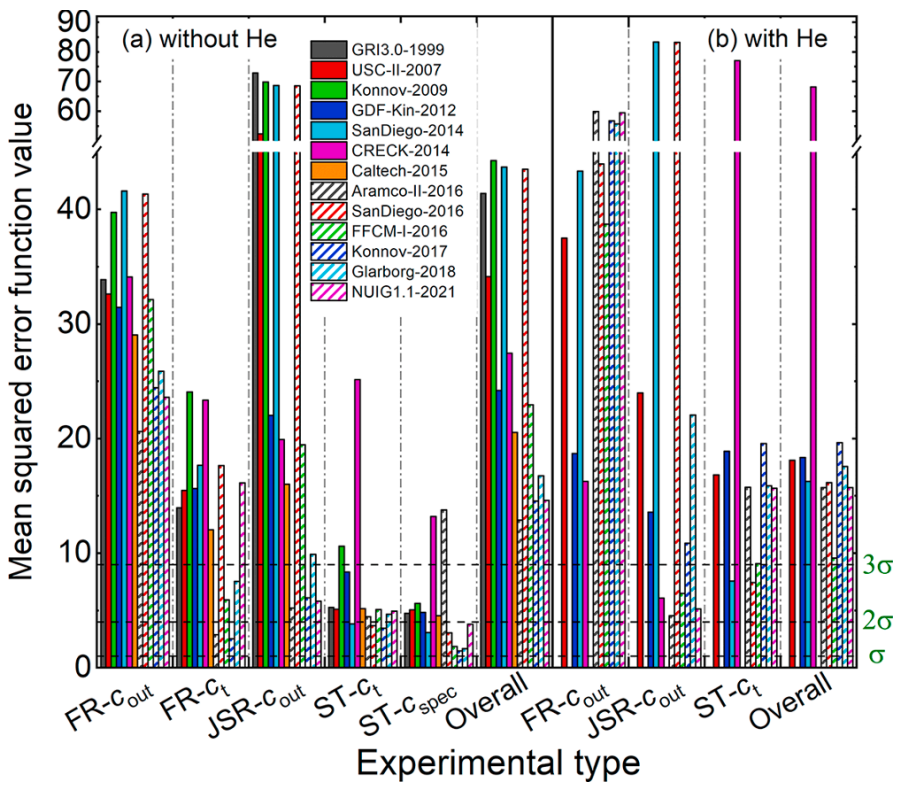
\includegraphics[width=0.65\linewidth]{img/sonstiges/Mechanismusvergleich_Zhang.png}
                \caption{Mittlerer quadrierter Fehler verschiedener Reaktionsmechanismen in Simulationen ohne (a) und mit (b) Helium aus einer Vergleichsstudie \cite{ZHANG2025114499}.}
                \label{fig:mechanismusvergleich_zhang}
            \end{figure} 
            Aufgrund der großen Menge an Daten in Abbildung \ref{fig:mechanismusvergleich_zhang} werden ausgewählte Zahlenwerte in Tabelle \ref{tab:zhang_mechanismen_auszug} dargestellt.
            \begin{table}[H]
                \centering
                \caption{Auszug aus den mittleren quadratischen Fehlerwerten (Mean Squared Error Function Values) verschiedener Mechanismen ohne Helium nach \textcite{ZHANG2025114499}.}
                \begin{tabular}{lcccccc}
                \toprule
                Mechanismus & FR$_\text{out}$ & FR$_\text{t}$ & JSR$_\text{out}$ & ST$_\text{t}$ & ST$_\text{spec}$ & Overall \\
                \midrule
                GRI3.0--1999   & 33.87 & 13.96 & 72.90 & 5.25 & 4.75 & 41.39 \\
                CRECK--2014    & 34.10 & 23.37 & 19.91 & 15.24 & 13.20 & 27.46 \\
                Aramco--II--2016 & 20.60 & 2.87 & 5.20 & 4.43 & 13.76 & 12.86 \\
                NUIG1.1--2021  & 23.59 & 16.12 & 5.79 & 4.94 & 3.81 & 14.61 \\
                \bottomrule
                \end{tabular}
                \label{tab:zhang_mechanismen_auszug}
            \end{table}
            Als Ergebnis dieser Studie wird Aramco-II-16 als zuverlässigster Reaktionsmechanismus genannt \cite{ZHANG2025114499}. 

            Zettervall et al. untersuchten die Anwendbarkeit von Reaktionsmechanismen für CFD-Analysen und fanden, dass Aramco die besten Ergebnisse liefert. Da CFD-Simulationen allerdings einen deutlich höheren Rechenbedarf erfordern, muss für die Anwendung dieses Mechanismus dieser stark reduziert werden. Insgesamt zeigt diese Studie jedoch, dass die meisten Mechanismen vergleichbare Ergebnisse liefern \cite{fuels2020013}. 

            In der Literatur finden sich nur wenige Arbeiten, die sich explizit mit der numerischen Effizienz chemischer Reaktionsmechanismen befassen. Der Einfluss der Komplexität des Mechanismus, insbesondere die Anzahl der Spezies und Elementarreaktionen, auf den Rechenaufwand wird meist nur theoretisch beschrieben \parencite{Niemeyer2016, CURTIS2017312}, eine systematische Quantifizierung anhand praktischer Simulationen ist jedoch selten, speziell im Gebiet der partiellen Oxidation. 
            Eine solche Analyse bietet hohes Potenzial, um Mechanismen nicht nur hinsichtlich ihrer berechneten Ergebnisse, sondern auch hinsichtlich ihrer Recheneffizienz zu beurteilen. 

            Zusammenfassend lässt sich feststellen, dass alle Reaktionsmechanismen ähnliche Ergebnisse liefern. Obwohl einige Studien die Verbrennungscharakteristiken von Methan untersuchen, ist eine Übertragbarkeit auf die partielle Oxidation möglich. Alle aufgeführten Mechanismen wurden zusätzlich unter den Bedingungen der hier betrachteten Versuchsanlage validiert. Insbesondere die Vergleichsstudie deutet darauf hin, dass der Reaktionsmechanismus Aramco tendenziell den geringsten Fehler aufweist. Dabei bietet Aramco zudem einen guten Kompromiss aus Genauigkeit, Detaillierungsgrad und Rechenaufwand.
    \chapter{Experimentelle Grundlagen und Rahmenbedingungen}
    Forschungsgegenstand ist ein Reaktor, der im Rahmen des Verbundvorhabens $\mbox{SCOORE}$ (\textit{Synthesis gas from recycling of CO$_2$}) genutzt wurde. Ziel dieses Projekts ist es, eine CO$_2$-verbrauchende Synthesegasherstellung zu untersuchen und damit einen Beitrag zur Reduzierung der Treibhausgasemissionen in der chemischen Industrie zu leisten. 

    Das Vorhaben wird von der BASF~SE in Kooperation mit der Technischen Universität Bergakademie Freiberg durchgeführt und zielt darauf ab, eine großtechnisch umsetzbare Prozessführung für die nichtkatalytische Partialoxidation von Erdgas in einer CO$_2$-reichen Atmosphäre zu entwickeln \cite{Scoore_Enargus}.  
    \section{Aufbau der Versuchsanlage und des Reaktors}
        Der untersuchte Reaktor ist als zylindrischer Hochdruckreaktor mit feuerfester Ausmauerung ausgeführt und besitzt eine Gesamtlänge von ca. 1,5~m bei einem Innendurchmesser von 0,36~m. Die Anlage ist für Betriebsdrücke bis 70~bar und maximale Temperaturen bis 1400~°C ausgelegt. Der Brenner ist als Mehrloch-Mischbrenner ausgeführt, der eine homogene Mischung der eintretenden Ströme ermöglicht. Dieser Mischbrenner wird mit Wasser gekühlt. In Abbildung \ref{fig:reaktorgeometrie} ist der Aufbau des Brenners sowie des gesamten Reaktors dargestellt. 
        \begin{figure}[H]
            \centering
            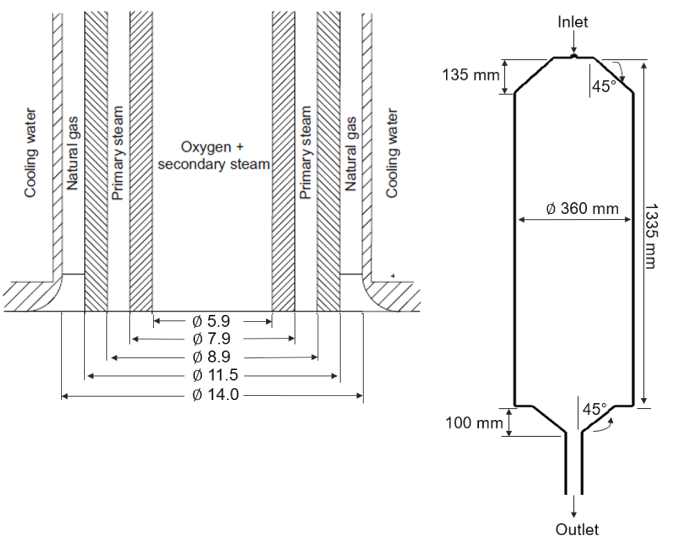
\includegraphics[width=0.6\linewidth]{img/sonstiges/Reaktorgeometrien.png}
            \caption{Geometrien des Reaktors sowie des Brenners}
            \label{fig:reaktorgeometrie}
        \end{figure}
    \section{Prozessbedingungen}
        Im Rahmen des Projekts wird der Prozess in zwei Varianten untersucht, um den Einfluss einer gezielten CO\textsubscript{2}-Zugabe auf die Reaktionsführung der nicht-katalytischen Hochdruck-Partialoxidation (HP-POx) von Erdgas systematisch zu bewerten. 
        
        Die erste Variante dient als Referenzprozess und beschreibt die konventionelle HP-POx von Erdgas unter Standardbedingungen ohne zusätzliche Zugabe von CO\textsubscript{2}. Dieser Fall repräsentiert den etablierten industriellen Prozess, bei dem Methan mit Sauerstoff und Wasserdampf unter stöchiometrisch limitierter Sauerstoffzufuhr zu einem Kohlenmonoxid- und wasserstoffhaltigen Synthesegas umgesetzt wird. 
        
        In der zweiten Variante wird der Reaktionsverlauf unter vergleichbaren thermischen und stofflichen Betriebsbedingungen untersucht, jedoch mit einem zusätzlichen CO\textsubscript{2}-Feed im Zulauf. Durch die Einmischung von CO\textsubscript{2} verändert sich das lokale Reaktionsgleichgewicht sowie die Temperaturführung im Reaktor, wodurch sich sowohl kinetische als auch thermodynamische Effekte ergeben. 
        
        Der Vergleich beider Prozessführungen erlaubt Rückschlüsse auf den Einfluss des CO\textsubscript{2}-Gehalts auf die chemische Umwandlung der Reaktanden sowie die Zusammensetzung des Produktgases. Darüber hinaus wird untersucht, inwieweit die CO\textsubscript{2}-Zugabe zur Reduktion der Netto-CO\textsubscript{2}-Emissionen beiträgt und welche Anpassungen an Betriebsparametern für eine stabile Prozessführung erforderlich sind.  
        
        In Tabelle \ref{tab:rahmenbedingungen_versuche} sind die wesentlichen Prozessparameter und Betriebsbedingungen der beiden Fälle zusammengefasst. Es ist ersichtlich, dass bei der CO\textsubscript{2}-Variante ein zusätzlicher Stoffstrom von etwa 196~kg/h Kohlenstoffdioxid in den Reaktor eingespeist wurde, während die übrigen Einsatzströme in Temperatur und Massenstrom nur geringfügig voneinander abweichen. Der Reaktor selbst weist ein Volumen von  134~Litern auf und wird unter stationären Bedingungen betrieben, wobei ein konstanter Wandwärmeverlust von etwa 30~kW berücksichtigt wird.
        
        \begin{table}[H]
            \centering
            \caption{Vergleich der Prozessfälle \cite{gonzales}}
            \label{tab:rahmenbedingungen_versuche}
            \begin{tabular}{llll}
            \toprule
            \textbf{Variablen} & & \textbf{Fall 1} & \textbf{Fall 2} \\
            \midrule
            \textbf{1. Erdgas} & Temperatur [°C] & 66,6 & 67,5 \\
                               & Massenstrom [kg/h] & 182,4 & 153,3 \\
            \midrule
            \textbf{2. Kohlenstoffdioxid} & Temperatur [°C] & -- & 67,5 \\
                                     & Massenstrom [kg/h] & 0 & 196,4 \\
            \midrule
            \textbf{3. Sauerstoff} & Temperatur [°C] & 231,9 & 231,2 \\
                                   & Massenstrom [kg/h] & 252,2 & 246,9 \\
            \midrule
            \textbf{4. Dampf} & Temperatur [°C] & 353,4 & 353,4 \\
                              & Massenstrom [kg/h] & 38,7 & 39,4 \\
            \midrule
            Wandwärmeverlust [kW] & & 30 & 30 \\
            Reaktorvolumen [L] & & 134 & 134 \\
            Druck [bar] && 47 & 47\\
            \midrule
            \textbf{Bemerkung} & & Referenz & CO\textsubscript{2}-Zugabe \\
            \bottomrule
            \end{tabular}
        \end{table}
        
    \section{Messverfahren und Messwerte}
        Entlang der Reaktorlängsachse sind mehrere Thermoelemente installiert, die die axiale Temperaturverteilung im Reaktor ermitteln. Zusätzlich sind Druck- und Massenstromsensoren in die Zuleitungen integriert, um die Prozessbedingungen konstant überwachen zu können. Das Produktgas wird am Reaktorausgang über eine gekühlte Probenahmeeinheit entnommen und anschließend gasanalytisch untersucht, wobei insbesondere die Volumenanteile von Wasserstoff, Kohlenstoffmonoxid, Kohlenstoffdioxid, Methan und Wasserdampf bestimmt werden \cite{RICHTER2015110}. Abbildung \ref{fig:erweiterungen_messpunkte} zeigt die Positionen der relevanten Thermoelemente. 
        \begin{figure}[H]
            \centering
            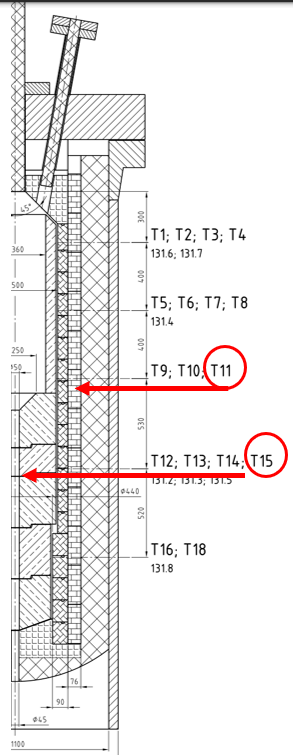
\includegraphics[width=0.2\linewidth]{img/Erweiterungen/Messpunkte.png}
            \caption{Messpunkte im Reaktor \cite{gonzales}}
            \label{fig:erweiterungen_messpunkte}
        \end{figure}
        Um die stofflichen Zusammensetzungen zu ermitteln, werden Infrarot-Absorptions\-spek\-troskopie (NDIR) und Wärmeleitfähigkeitsmessung (TCD) eingesetzt. Die ermittelten Daten der Zusammensetzung des Synthesegases und die Temperaturen beider Prozessbedingungen sind in Tabelle \ref{tab:messwerte} dargestellt. 
        \begin{table}[H]
            \centering
            \caption{Experimentelle Ergebnisse der Synthesegaszusammensetzungen sowie der Temperaturmessungen und Massenströme beider Betriebsweisen \cite{gonzales}}
            \label{tab:messwerte}
            \begin{tabular}{l l c c}
            \toprule
             & \textbf{Einheit} & \textbf{Fall 1 (Referenz)} & \textbf{Fall 2 (CO\textsubscript{2}-Zugabe)} \\
            \midrule
            Synthesegas (nass) & kg/s & 0{,}13 & 0{,}18 \\
            Temperatur Austritt & °C & (1300)\textsuperscript{*} & (1342)\textsuperscript{*} \\
            Temperatur T102.11 & °C & 1407{,}4 & 1411{,}4 \\
            Temperatur T102.15 & °C & 1351{,}9 & 1371{,}6 \\
            \midrule
            H\textsubscript{2} & Vol.-\% trocken & 0{,}599 & 0{,}416 \\
            CO & Vol.-\% trocken & 0{,}341 & 0{,}416 \\
            CH\textsubscript{4} & Vol.-\% trocken & 0{,}007 & 0{,}0012 \\
            CO\textsubscript{2} & Vol.-\% trocken & 0{,}048 & 0{,}151 \\
            \midrule
            H\textsubscript{2}/CO & – & 1{,}751 & 0{,}981 \\
            \bottomrule
            \end{tabular}
            \footnotesize{*~Werte in Klammern wurden mit \textit{Aspen Plus} berechnet und stellen keinen Experimentalwert dar.}
        \end{table}
    \section{Vorbetrachtungen}
        \label{sec:vorbetrachtungen}
        Zur Vorbereitung der Modellierungsarbeiten liegen bereits umfangreiche CFD-Analysen sowie ein darauf basierendes komplexes Reaktornetzwerk-Modell (ROM) aus dem Projekt SCOORE vor. Diese Untersuchungen bilden die Grundlage für das Verständnis der Strömungs- und Reaktionsvorgänge innerhalb des betrachteten POx-Reaktors \cite{gonzales}. 
        
        %Die CFD-Simulationen wurden unter stationären Bedingungen mit detaillierter Berücksichtigung der Strömungs- und Temperaturfelder durchgeführt. Auf Basis dieser Ergebnisse erfolgte eine Segmentierung des Reaktors in charakteristische Zonen, die durch idealisierte Reaktoren beschrieben werden können. 
        %In Abbildung \ref{fig:reaktorsegmentierung} ist die CFD-basierte Segmentierung des Reaktors dargestellt, aus der das bestehende Netzwerk aus Perfectly Stirred Reactors (PSR) und Plug Flow Reactors (PFR) abgeleitet wurde.
        Die CFD-Simulation wurde unter stationären Bedingungen mit detaillierter Berücksichtigung der Strömungs- und Temperaturfelder durchgeführt. Dabei konnte der Reaktor in charakteristische Strömungszonen segmentiert werden, die sich untereinander durch verschiedene Reaktions- und Mischcharakteristiken auszeichnen. Auf Basis dieser Simulation erfolgte die konzeptionelle Erstellung des komplexen ROMs, das PFR- und PSR- Elemente enthält. Diese Segmentierung ermöglicht eine deutliche Vereinfachung der Berechnung dieses Reaktors. 
        
        \begin{figure}[H]
            \centering
            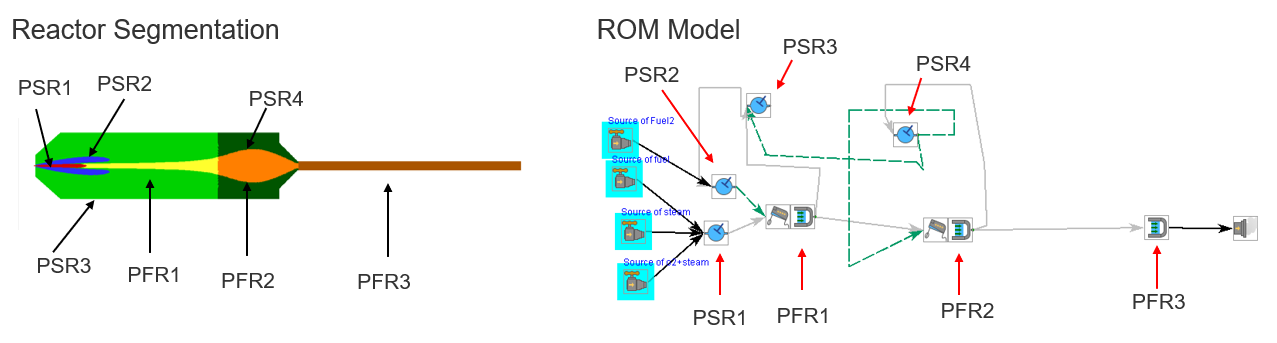
\includegraphics[width=1\linewidth]{img/sonstiges/Reactor Segmentation.png}
            \caption{Reaktorsegmentierung und komplexes ROM auf Basis einer CFD-Simulation \cite{gonzales}}
            \label{fig:reaktorsegmentierung}
        \end{figure}
        
    \chapter{Vergleich von Reaktionsmechanismen}
    Wie in Kapitel \ref{sec:reaktionsmechanismen_literatur} beschrieben, existiert eine Vielzahl von Reaktionsmechanismen, die sich hinsichtlich ihres Detaillierungsgrads und der Anzahl enthaltener Spezies und Elementarreaktionen deutlich unterscheiden. Die Komplexität eines Mechanismus beeinflusst maßgeblich den Bedarf der Rechenleistung und somit die Effizienz von Parameterstudien. 
    Da die meisten Reaktionsmechanismen ursprünglich für Verbrennungsprozesse entwickelt und validiert wurden, ist ein Vergleich ihrer Eignung für die Modellierung der partiellen Oxidation erforderlich. 
    \section{Überblick über die Reaktionsmechanismen}
    Als Grundlage der Modellierung chemischer Reaktionen nutzt Chemkin Datensätze für Reaktionsmechanismen. Es gibt verschiedene Datensätze, die sich in der Anzahl der Spezies sowie der Elementarreaktionen unterscheiden. In Tabelle \ref{tab:reaktionsmechanismen_überblick} sind die in dieser Arbeit genutzten Reaktionsmechanismen aufgelistet. 
    \begin{table}[H]
        \centering
        \caption{Überblick über Anzahl der Spezies sowie Reaktionen verschiedener Reaktionsmechanismen}
        \begin{tabular}{lcc}
        \toprule
        \textbf{Reaktionsmechanismus} & \textbf{Anzahl Spezies} & \textbf{Anzahl Reaktionen} \\
        \midrule
        ATR (in-house) & 28 & 112 \\
        GRI3.0         & 53 & 325 \\
        Aramco2.0      & 581 & 3037 \\
        NUIG1.1        & 2746 & 11270 \\
        CRECK *          & 159 & 2459 \\
        \bottomrule
        \end{tabular}
        \footnotesize{\\ *~bezieht sich auf den in der Arbeit verwendeten Mechanismus.}
        \label{tab:reaktionsmechanismen_überblick}
        
    \end{table}
    \subsection*{ATR}
        Der ATR-Mechanismus (in-house) stellt einen stark reduzierten Reaktionsmechanismus dar, der vor allem in komplexen Strömungssimulationen (CFD) eingesetzt wird. Aufgrund der geringen Anzahl an Spezies und Reaktionen bildet er ausschließlich die wesent\-lichen Hauptreaktionen der partiellen Oxidation von Methan bzw. Erdgas ab. Dies führt zu einer deutlich reduzierten Rechenzeit und ermöglicht den Einsatz in großskaligen Reaktornetzwerken oder gekoppelten CFD-Simulationen. Allerdings können mit diesem Mechanismus keine detaillierten chemischen Prozesse wie Nebenreaktionen, radikalische Zwischenprodukte oder Emissionspfade (z. B. NO$_x$-Bildung) erfasst werden, wodurch seine Anwendung auf vereinfachte Modellstudien beschränkt ist.
    \subsection*{GRI-Mech 3.0}
        GRI-Mech 3.0 ist ein detaillierter Reaktionsmechanismus, der ursprünglich im Rahmen des \emph{Gas Research Institute (GRI)} entwickelt wurde, um die Verbrennung von Methan und Erdgas realistisch zu beschreiben. Er umfasst 53 Spezies und 325 Elementarreaktionen und ist für die Hochtemperaturverbrennung sowie für die NO$_x$-Bildung optimiert \cite{Gri-Mech}.

        Der Mechanismus wurde umfassend anhand von Flammenexperimenten, Zündverzögerungszeiten und Emissionsmessungen validiert. In der Literatur gilt Gri-Mech oft als Referenzmechanismus und wird häufig für die Entwicklung von ROMs herangezogen. 

        Ein wesentlicher Vorteil von GRI-Mech ist sein geringer Umfang, wodurch der Mechanismus ähnlich wie ATR auch in Strömungssimulationen einsetzbar ist. Gleichzeitig enthält er ausreichend Reaktionspfade, um wichtige Phänomene korrekt nachzubilden. Einschränkungen bestehen jedoch bei höheren Kohlenwasserstoffen (ab C$_3$ - C$_4$), sowie im Niedertemperaturbereich.
    \subsection*{AramcoMech 2.0}
        Der AramcoMech 2.0 Reaktionsmechanismus ist ein Mechanismus mit einem hohen Detailgrad. Er wurde von der National University of Galway in Zusammenarbeit mit Saudi Aramco entwickelt. Dieser Mechanismus umfasst 581 Spezies und mehr als 3000 elementare Reaktionen und ist insbesondere auf die Oxidation und Verbrennung von kurzkettigen Kohlenwasserstoffen optimiert \cite{Aramco20}. 

        Der Mechanismus wurde umfassend anhand von  Zündverzögerungszeiten, laminaren Flammengeschwindigkeiten sowie Species-Profilen validiert. Dabei deckt diese einen breiten Bereich an Bedingungen ab, darunter hohe Drücke und Temperaturen. Damit ist AramcoMech 2.0 für die Simulation von technisch relevanten Verbrennungsprozessen geeignet, bei denen neben Methan auch andere Stoffe wie Ethan, Ethen, Propan und Propen eine Rolle spielen. 

        Durch den deutlich höheren Detailgrad dieses Mechanismus ist die Verwendung desselben in CFD-Simulationen sehr rechenintensiv. 
    \subsection*{NUIGMech1.1}
        NUIGMech 1.1 ist ein sehr detaillierter Reaktionsmechanismus, der über 2500 Spezies und über 11000 Elementarreaktionen umfasst. Damit zählt er zu den umfangreichsten Mechanismen für die Verbrennung und Oxidation von Kohlenwasserstoffen \cite{MARTINEZ2021401}.

        Der Mechanismus wurde in einer Vielzahl von Experimenten validiert. Abgedeckt wird ein breites Spektrum an Bedingungen, darunter hohe Temperaturen, hohe Drücke und breite Äquivalenzverhältnisse. 

        Im Gegensatz zu anderen Reaktionsmechanismen unterstützt NUIGMech 1.1 weitaus mehr Brennstoffe. Validierungen wurden unter anderem für die Oxidation von Methan und Ethan, für Erdgasgemische sowie für Propan/Propen und Propin, sowie für C$_2$-C$_6$ Alkane durchgeführt \cite{MARTINEZ2021401}. Dadurch können mit diesem Mechanismus Verbrennungen modelliert werden, bei denen komplexere Brennstoffe zum Einsatz kommen. 

        Die hohe Anzahl an Spezies und Reaktionen bringt jedoch einen erheblichen Rechenaufwand mit sich. So ist der Einsatz in CFD-Simulationen nicht praktikabel. Zudem treten bei komplexeren Reaktornetzwerken oftmals Divergenzprobleme und Instabilitäten auf.
    \subsection*{CRECK Mechanismus}
        Die Creck Modeling Group hat eine Vielzahl von Reaktionsmechanismen für verschiedene Anwendungsfälle und mit unterschiedlichem Detailgrad erstellt. Komplexe Mechanismen sind dabei für die Verbrennung von C$_1$ - C$_{16}$ Alkanen bei hohen und niedrigen Temperaturen sowie für die Bildung von NO$_x$ und Ruß verantwortlich. Ein besonderer Fokus liegt auf der Bildung von Schadstoffen sowie der Betrachtung von Aromaten im Verbrennungsprozess. Es existieren sowohl sehr kompakte (62 Elementarreaktionen), als auch sehr umfangreiche (27000 Elementarreaktionen) Mechanismen \cite{CRECK_DetailedMechanisms}.
    \section{Einfluss der Mechanismusgröße auf den Rechenaufwand}
        Die Rechenzeit bei Simulationen hängt wesentlich von der Größe des verwendeten Reaktionsmechanismus ab. Dabei bestimmen vor allem die Anzahl der chemischen Spezi\-es $N_s$ und der Elementarreaktionen $N_r$ die Komplexität der numerischen Lösung. Wie in Kapitel \ref{sec:theoretische_grundlagen} beschrieben, wird für jede Spezies eine Stoffbilanzgleichung gelöst. Somit ist die Dimension des Gleichungssystems gleich der Anzahl der im Mechanismus vorhandenen Spezies. Die Berechnung der Reaktionsraten erfolgt für jede Elementarreaktion separat auf Basis der Arrhenius-Gleichung (siehe Gleichung \ref{eq:Arrhenius}), wodurch der Aufwand zur Auswertung der rechten Seiten (RHS) in guter Näherung linear mit der Reaktionszahl $N_r$ skaliert \parencite{ChemkinTheoryManual, Niemeyer2016}.

        Wesentlich aufwändiger ist die Lösung der Differentialgleichungen. CHEMKIN verwendet hierfür implizite Integrationsverfahren (BDF, CVODE) und Newton-Verfahren für stationäre Lösungen, die in jeder Iteration ein Gleichungssystem der Dimension $N_s+1$ lösen. Im ungünstigsten Fall wächst der Rechenaufwand kubisch mit der Spezieszahl $t \sim \mathcal{O}\left(N_s^3\right)$, im besten Fall mit $t \sim \mathcal{O}\left(N_s^2\right)$ \cite{CURTIS2017312}.

        Da zwischen der Anzahl der Spezies und der Anzahl der Elementarreaktionen ein direkter Zusammenhang besteht, bewirkt eine Reduzierung der Speziesanzahl eine erhebliche Verkürzung der Laufzeit. Es ist daher von hohem Interesse, einen Reaktionsmechanismus zu wählen, der alle relevanten Spezies und Elementarreaktionen abdeckt und keine nicht relevanten Spezies enthält. %Beispielsweise wäre ein Mechanismus, der eine Vielzahl an längerkettigen Kohlenwasserstoffen berücksichtigt, \alert{keine gute Wahl für diesen Anwendungsfall.} %Wertend!
        So ist die Anwendung eines Reaktionsmechanismus für die Verbrennung von Erdgas redundant, wenn er umfangreiche Reaktionen langkettiger Kohlenwasserstoffe beschreibt. 
    % ---------- gehört in Auswertungskapitel --------------
\iffalse
    \section{Simulationen}
        \label{sec:Simulationen_reaktionsmechanismus}
        Für den Vergleich der Reaktionsmechanismen wurde die Partialoxidation in einem einfachen Reaktornetzwerk, bestehend aus einem PSR und einem PFR, modelliert. In diesem stellt der PSR die Flammzone, der PFR die Nachbrennzone dar. In Abbildung \ref{fig:rom_mechanismusvergleich} ist das Reaktornetzwerk schematisch dargestellt.\\
        \begin{figure}[htbp]
          \centering
          \tikzset{
            inletoutlet/.style={
              draw,
              rounded corners=2pt,
              fill=black!10,
              minimum height=10mm,
              minimum width=20mm,
              align=center
            },
            psr/.style={
              draw,
              circle,
              fill=blue!15,
              minimum size=12mm,
              align=center
            },
            pfr/.style={
              draw,
              rectangle,
              fill=blue!15,
              minimum height=10mm,
              minimum width=25mm,
              align=center
            },
            flow/.style={
              -{Stealth[length=2.2mm]},
              thick
            }
          }
        
          \begin{tikzpicture}[node distance=20mm, font=\small]
            % Nodes
            \node[inletoutlet] (inlet) {Inlet};
            \node[psr, right=of inlet] (psr) {PSR};
            \node[pfr, right=of psr] (pfr) {PFR};
            \node[inletoutlet, right=of pfr] (outlet) {Outlet};
        
            % Arrows
            \draw[flow] (inlet) -- (psr);
            \draw[flow] (psr) -- (pfr);
            \draw[flow] (pfr) -- (outlet);
          \end{tikzpicture}
        
          \caption{Schematische Darstellung der Prozessabfolge: Inlet → PSR → PFR → Outlet.}
          \label{fig:rom_mechanismusvergleich}
        \end{figure}
        \subsection{Simulation ohne CO$_2$}
        Über die Länge der Nachbrennzone lassen sich die Stoffmengenanteile aufteilen. In Abbildung \ref{fig:vergleich_h2_ch4_keinco2} sind beispielsweise die Stoffmengenanteile von Wasserstoff und Methan dargestellt.
        \begin{figure}[H]
            \centering
            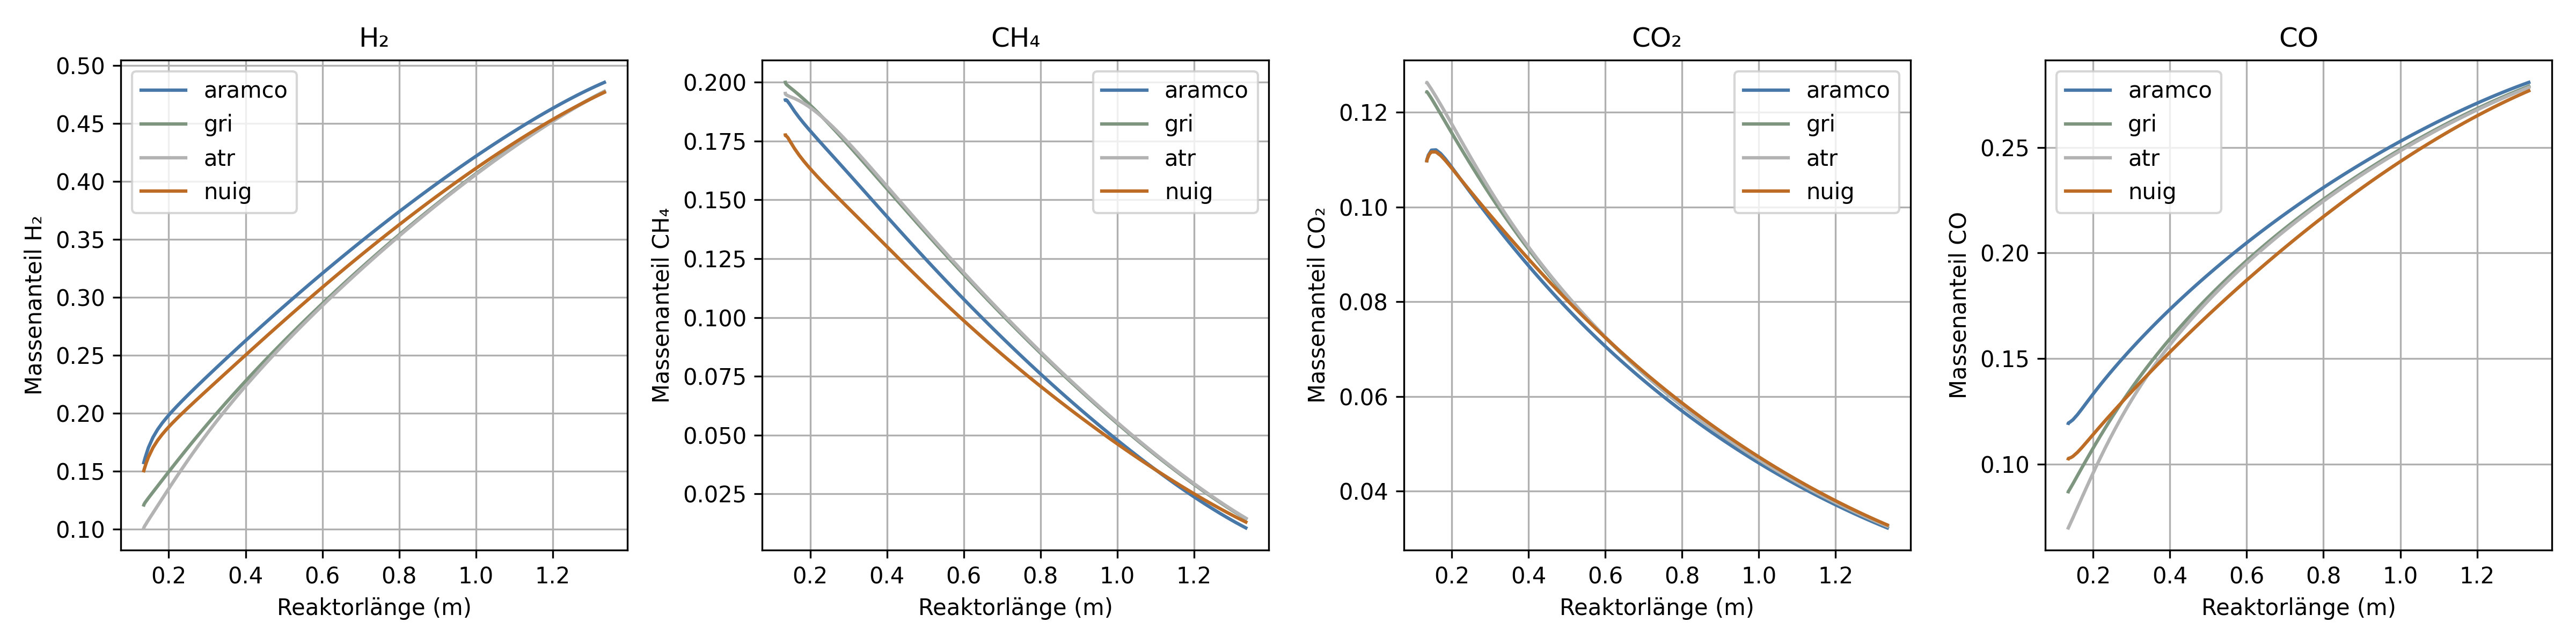
\includegraphics[width=1\linewidth]{img/Vergleich_mech/CO_CO2_keinCO2.png}
            \caption{Darstellung der Stoffmengenanteile Wasserstoff und Methan für die Simulation ohne CO$_2$}
            \label{fig:vergleich_h2_ch4_keinco2}
        \end{figure}
        Zwar zeigen sich kleine Unterschiede für die verschiedenen Reaktionsmechanismen, allerdings ähnelt sich der Verlauf immer stark. So ist die berechnete Zusammensetzung des Abgases annähernd identisch. In Tabelle \ref{tab:vergleich_abgaszusammensetzung_keinco2} sind die Ergebnisse der Simulationen sowie die experimentell vorliegenden Daten dargestellt. Dabei handelt es sich um trockengas, bei dem Wasserdampf entfernt worden ist. 
        \begin{table}[H]
            \centering
            \caption{Vergleich der Modell- und Experimentalwerte der Molenbrüche ohne CO\textsubscript{2}-Zugabe}
            \label{tab:vergleich_abgaszusammensetzung_keinco2}
            \begin{tabular}{lccccc}
                \toprule
                & \textbf{Exp.} & \textbf{GRI} & \textbf{ARAMCO} & \textbf{ATR} & \textbf{NUIG} \\
                \midrule
                \textbf{H$_2$} [Vol.-\%] & 0,599 & 0,594 & 0,600 & 0,594 & 0,596 \\
                \textbf{CO} [Vol.-\%]& 0,341 & 0,347 & 0,347 & 0,347 & 0,346 \\
                \textbf{CH$_4$} [Vol.-\%]& 0,007 & 0,018 & 0,013 & 0,018 & 0,016 \\
                \textbf{CO$_2$} [Vol.-\%]& 0,048 & 0,041 & 0,040 & 0,041 & 0,041 \\
                \bottomrule
            \end{tabular}
        \end{table}
        Die erhaltenen Werte weisen eine hohe Ähnlichkeit zu den experimentell ermittelten Werten auf, wobei es jedoch leichte Abweichungen beim Methan und Kohlenstoffdioxid gibt. 
        \subsection{Simulation mit CO$_2$}
        Analog zur Simulation ohne CO$_2$ werden die Stoffe über die Länge der Nachbrennzone analysiert (siehe Abbildung \ref{fig:vergleich_h2_ch4_co2}).
        \begin{figure}[H]
            \centering
            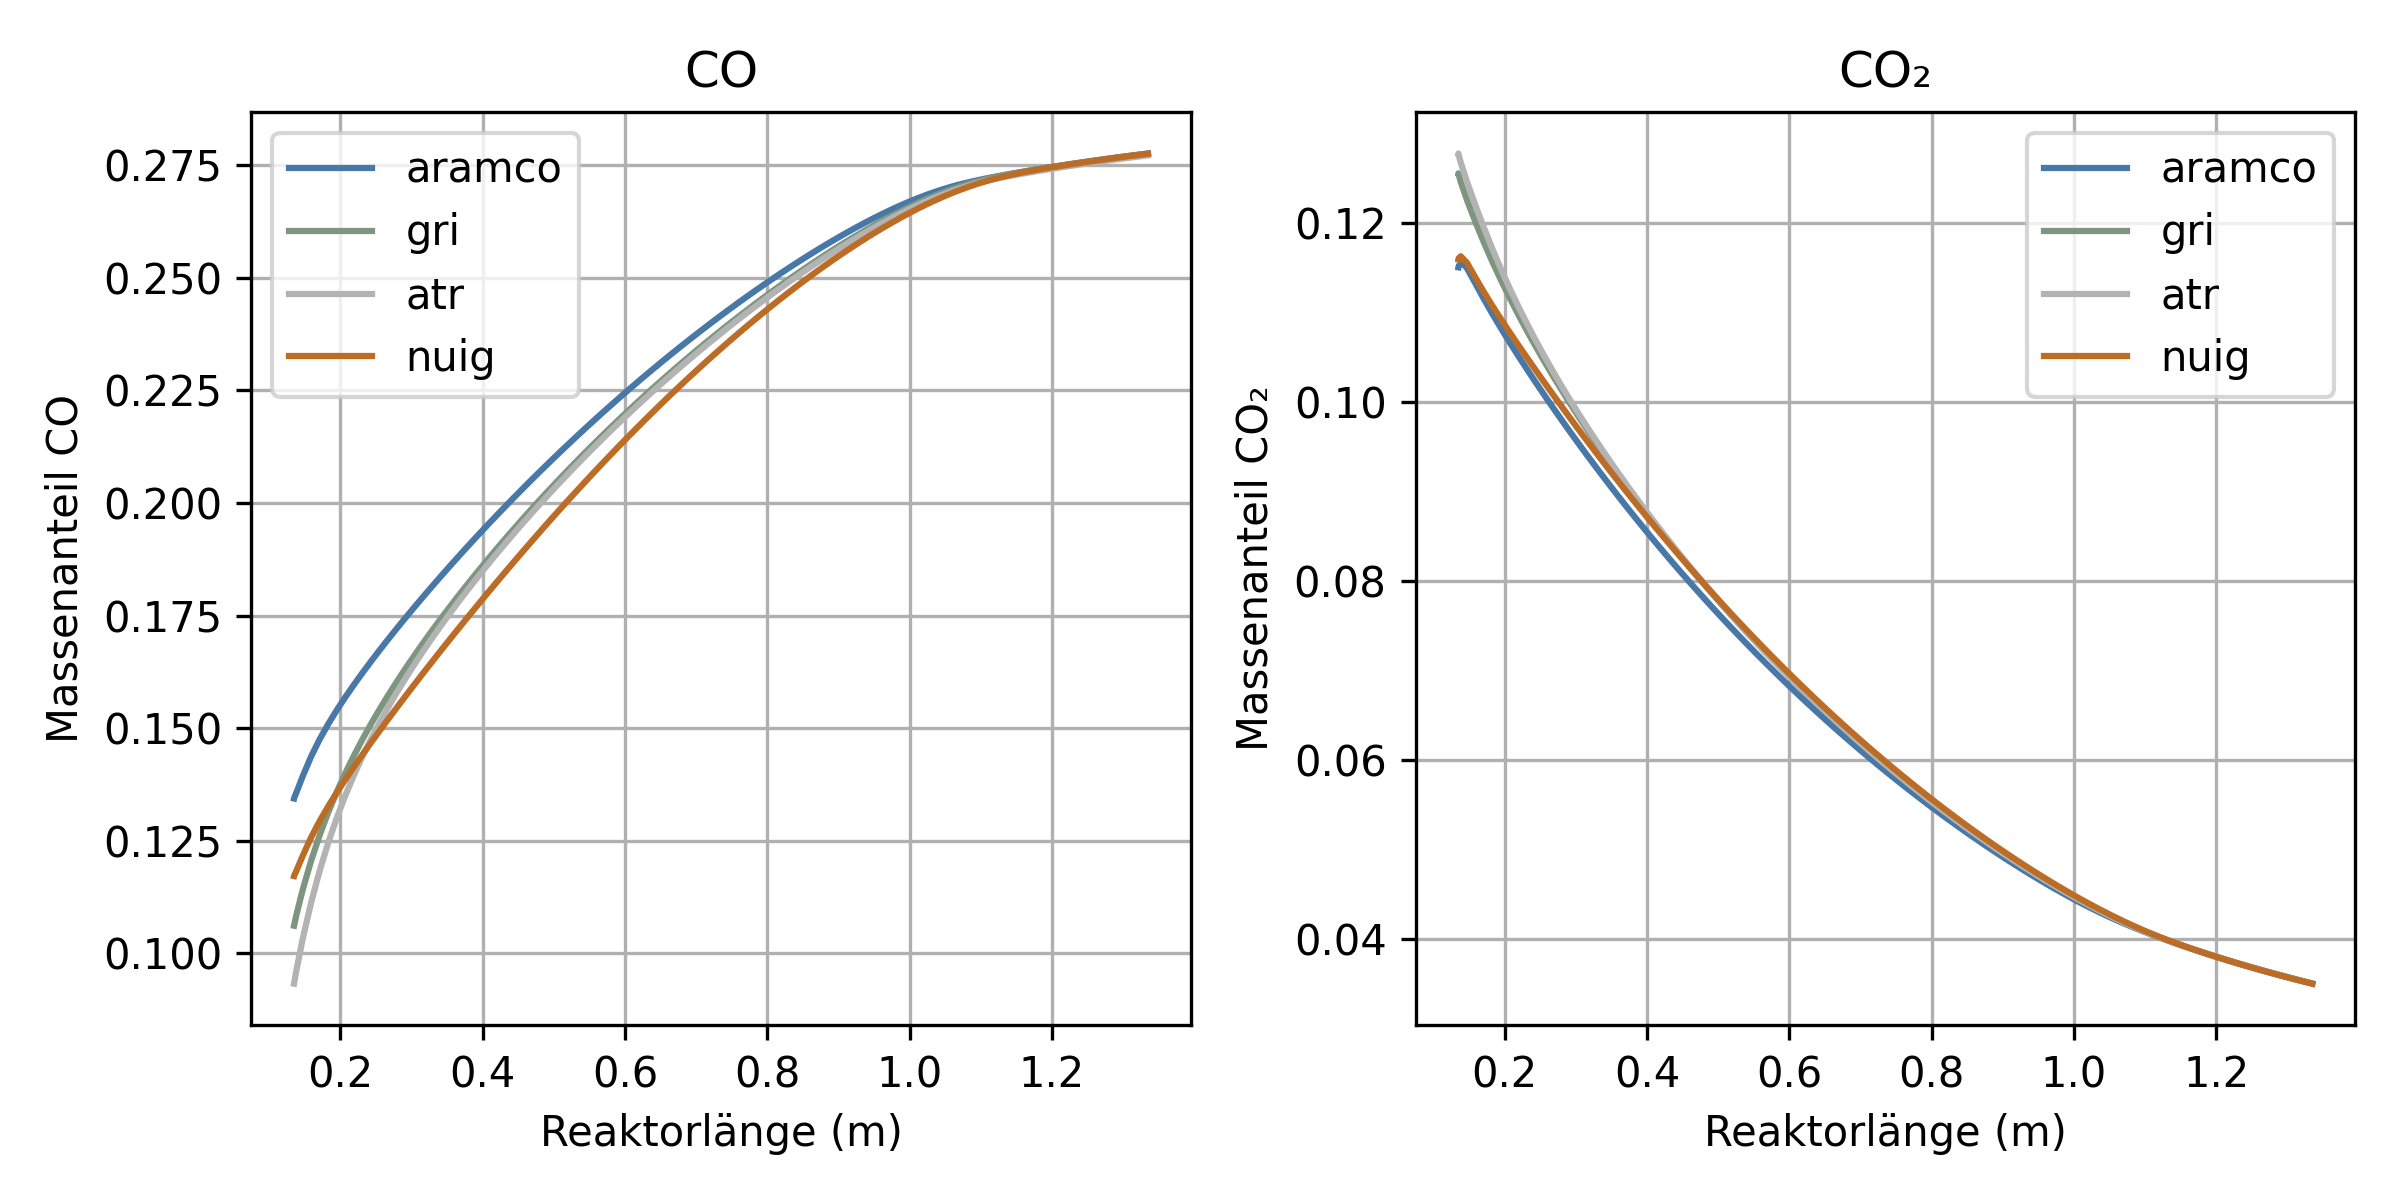
\includegraphics[width=1\linewidth]{img/Vergleich_mech/CO_CO2_CO2.png}
            \caption{Darstellung der Stoffmengenanteile Wasserstoff und Methan für die Simulation mit CO$_2$}
            \label{fig:vergleich_h2_ch4_co2}
        \end{figure}
        Auch hier zeichnet sich ein ähnliches Bild. Die Verläufe sind alle sehr ähnlich und führen zu sehr ähnlichen Abgaszusammensetzungen. In Tabelle sind die berechneten Stoffmengenanteile sowie die experimentell ermittelten Daten dargestellt (wie in Tabelle \ref{tab:vergleich_abgaszusammensetzung_keinco2}).
        \begin{table}[H]
            \centering
            \caption{Vergleich der Modell- und Experimentalwerte der Molenbrüche mit CO\textsubscript{2}-Zugabe}
            \begin{tabular}{lccccc}
                \toprule
                & \textbf{Exp.} & \textbf{GRI} & \textbf{ARAMCO} & \textbf{ATR} & \textbf{NUIG} \\
                \midrule
                \textbf{H$_2$} [Vol.-\%]& 0,416 & 0,579 & 0,579 & 0,580 & 0,579 \\
                \textbf{CO} [Vol.-\%]& 0,424 & 0,373 & 0,373 & 0,373 & 0,373 \\
                \textbf{CH$_4$} [Vol.-\%]& 0,001 & 0,000 & 0,000 & 0,000 & 0,000 \\
                \textbf{CO$_2$} [Vol.-\%]& 0,151 & 0,047 & 0,047 & 0,047 & 0,047 \\
                \bottomrule
            \end{tabular}
        \end{table}
        Im Vergleich zu den Ergebnissen der Simulation ohne Zugabe von Kohlenstoffdioxid weisen die simulierten Werte eine hohe Abweichung auf. Jedoch ergeben sich für alle Reaktionsmechanismen die gleichen Werte. \alert{Systematischer Fehler!}
\fi 
    \chapter{Parameterstudie CO\textsubscript{2}}
\iffalse 
    \section{Simulation der Parameterstudie}
    Um den Einfluss von einer Zugabe an Kohlenstoffdioxid zu verstehen, wurde eine Parameterstudie durchgeführt. Dabei wurde analog zum Vergleich der Reaktionsmechanismen das in Abbildung \ref{fig:rom_mechanismusvergleich} dargestellte ROM genutzt. Dabei wurde der Einlass an Kohlenstoffdioxid von minimal 0~kg/s bis maximal 0,2~kg/s variiert. Alle anderen Prozessparameter wurden dabei nicht verändert. 
    \section{Ergebnisse der Parameterstudie}
    In Abbildung \ref{fig:parameterstudie_temperaturen} sind die in der Simulation bestimmten Maximal- sowie Minimaltemperaturen für die Parameterstudie dargestellt
    \begin{figure}[H]
        \centering
        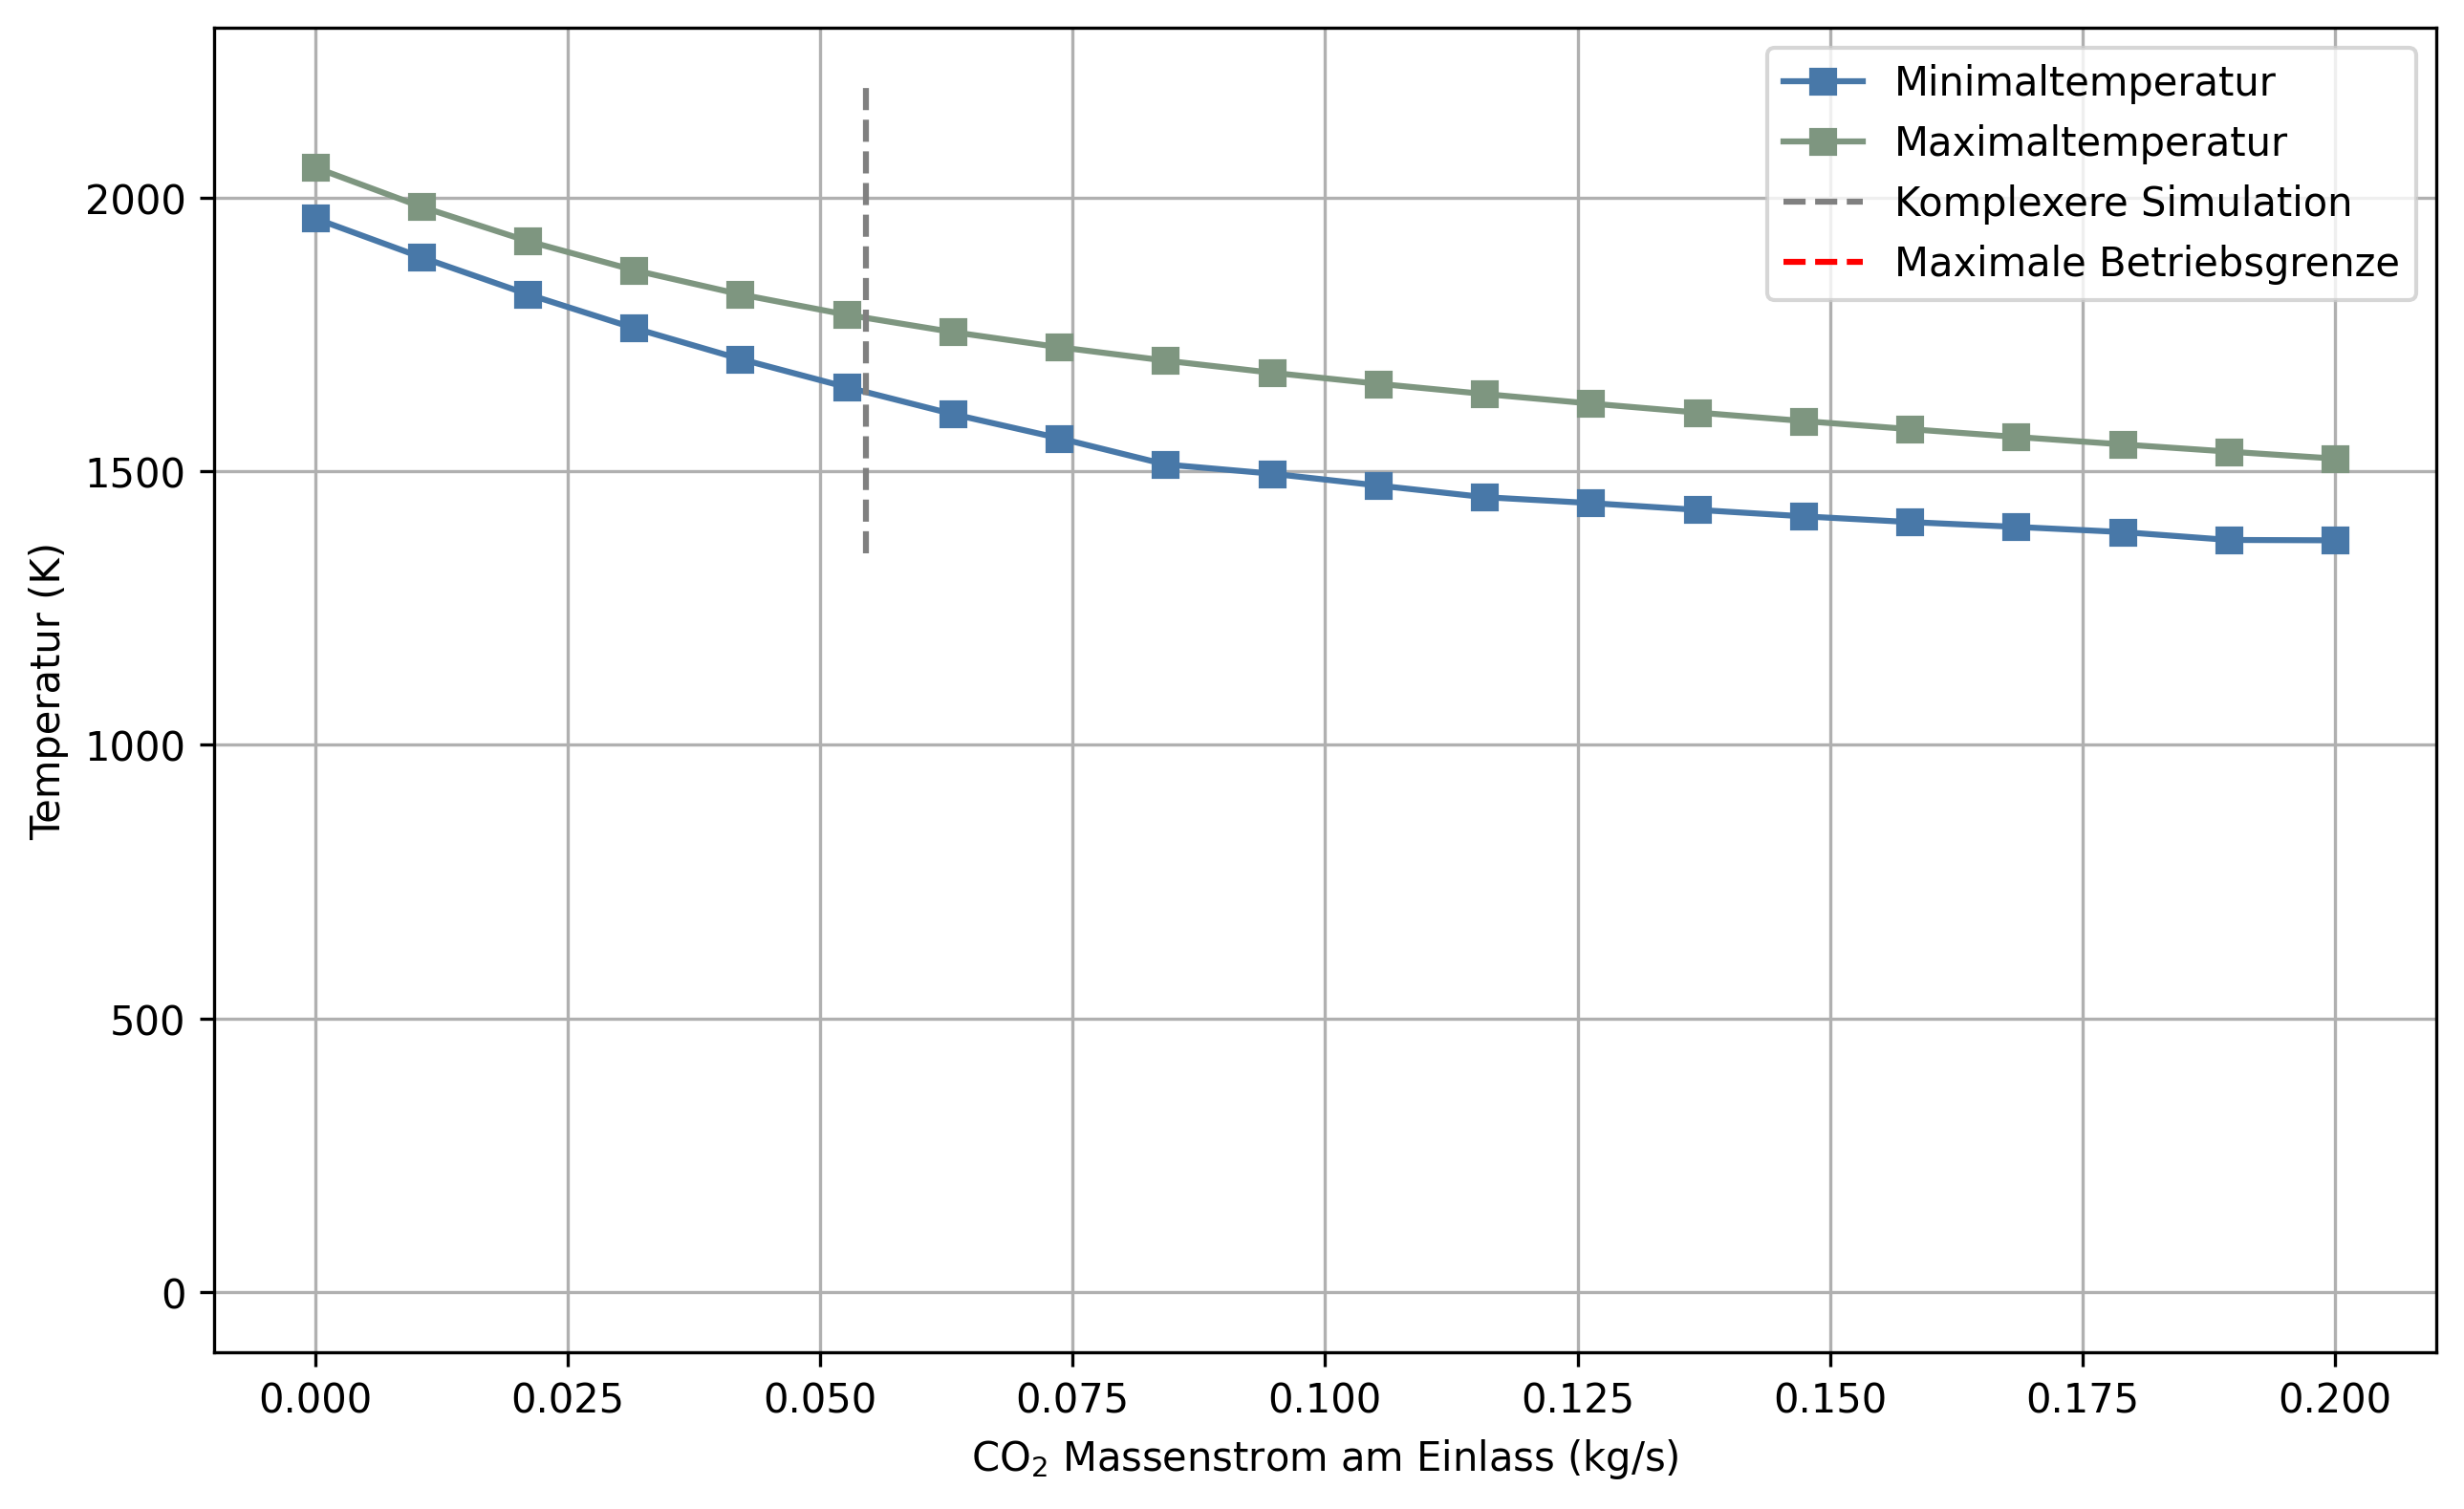
\includegraphics[width=0.9\linewidth]{img/Parameterstudie_CO2/Parameterstudie_CO2_Temperaturen.png}
        \caption{Simulierte maximale und minimale Temperatur im Reaktor (PFR)}
        \label{fig:parameterstudie_temperaturen}
    \end{figure}
    Die Temperaturverläufe im Reaktor zeigen, dass sowohl die maximale als auch die minimale Temperatur mit steigendem CO$_2$-Massenstrom am Einlass deutlich abnehmen. Während im Betrieb ohne CO$_2$ Temperaturen von über 2000j~K erreicht werden, sinkt die Reaktionstemperatur bei hoher CO$_2$ Zufuhr auf Werte um 1500~K. Diese Beobachtung ist durch zwei Effekte erklärbar. Zum einen wirkt 
    CO$_2$ aufgrund seiner hohen Wärmekapazität als Verdünnungsgas, das die Temperaturen der exothermen Oxidationsreaktionen absenkt \cite{NIST_CO2_WebBook_General}. Zum anderen fördern zusätzliche Mengen an CO$_2$ endotherme Reformierungsreaktionen, die weitere Wärme aufnehmen und damit den Temperaturgang zusätzlich abflachen. In Folge steht für die Umsetzung der Brennstoffkomponenten weniger Energie zur Verfügung. 

    In Abbildung \ref{fig:parameterstudie_massenströme} sind die Massenströme am Reaktorausgang als Ergebnis der Parameterstudie dargestellt. 
    \begin{figure}[H]
        \centering
        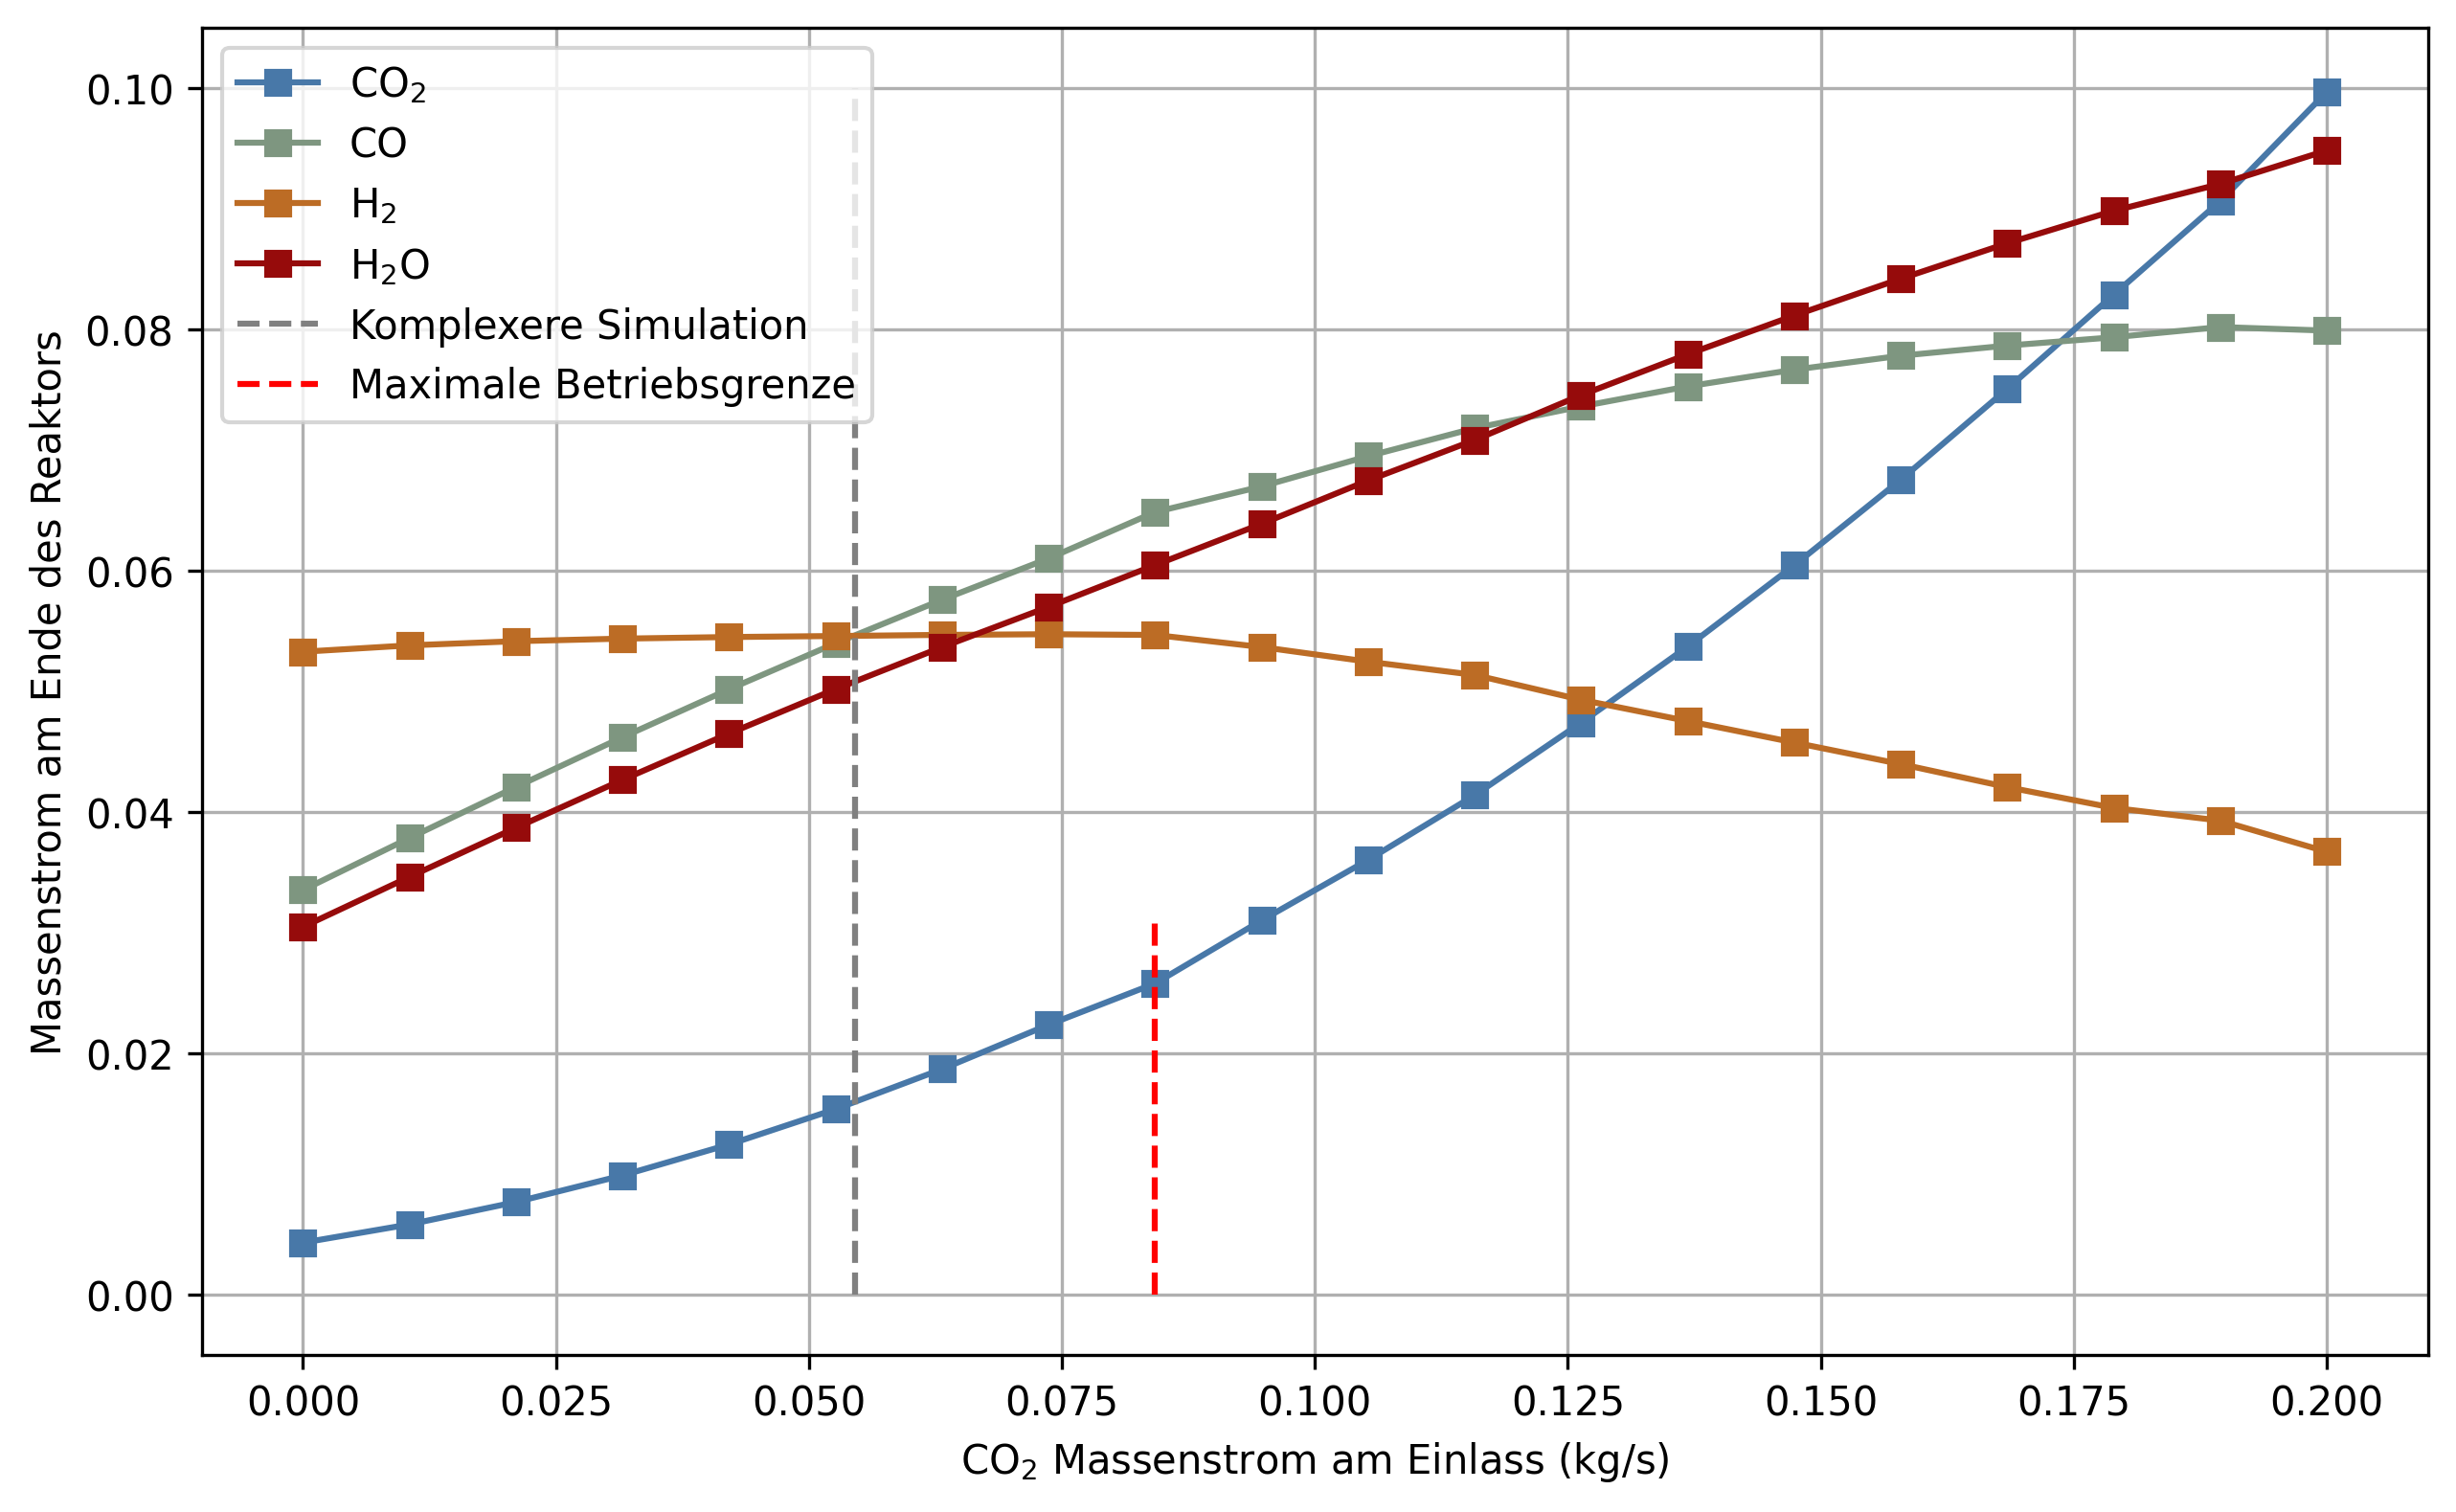
\includegraphics[width=0.9\linewidth]{img/Parameterstudie_CO2/Parameterstudie_CO2_Massenstrom_Ende.png}
        \caption{Simulierte Massenströme von CO$_2$, CO, H$_2$ und H$_2$O am Reaktorausgang der Parameterstudie}
        \label{fig:parameterstudie_massenströme}
    \end{figure}
    Der beobachtete Temperaturabfall spiegelt sich unmittelbar in den erhaltenen Massenströmen wider. Besonders auffälliges Verhalten zeigt dabei der Wasserstoff. Während dieser bei niedrigen Temperaturen annähernd konstant bleibt, nimmt er bei steigendem CO$_2$-Massenstrom deutlich ab. Die sinkenden Temperaturen bremsen die Wasserstoffbildung in den endothermen Reformierungereaktionen, sodass weniger Wasserstoff produziert wird. Gleichzeitig verschiebt sich die Gleichgewichtslage der Wassergas-Shift-Reaktion (siehe Gleichung \ref{eq:wassergas_shift}) in entgegengesetzte Richtung, wodurch zusätzlich Wasserstoff verbraucht wird. Parallel dazu steigen die Ströme von CO$_2$ und H$_2$O an, während CO zunächst zunimmt, sich dann jedoch einem konstanten Massenstrom annähert, was auf die Kombination thermodynamischer und kinetischer Limitierungen zurückzuführen ist. 

    Die Darstellung der Stoffmengenanteile (Abbildung \ref{fig:parameterstudie_molenbruch}) zeigt eine deutliche Verschiebung der Produktzusammensetzung mit zunehmendem CO$_2$ Massenstrom. 
    \begin{figure}[H]
        \centering
        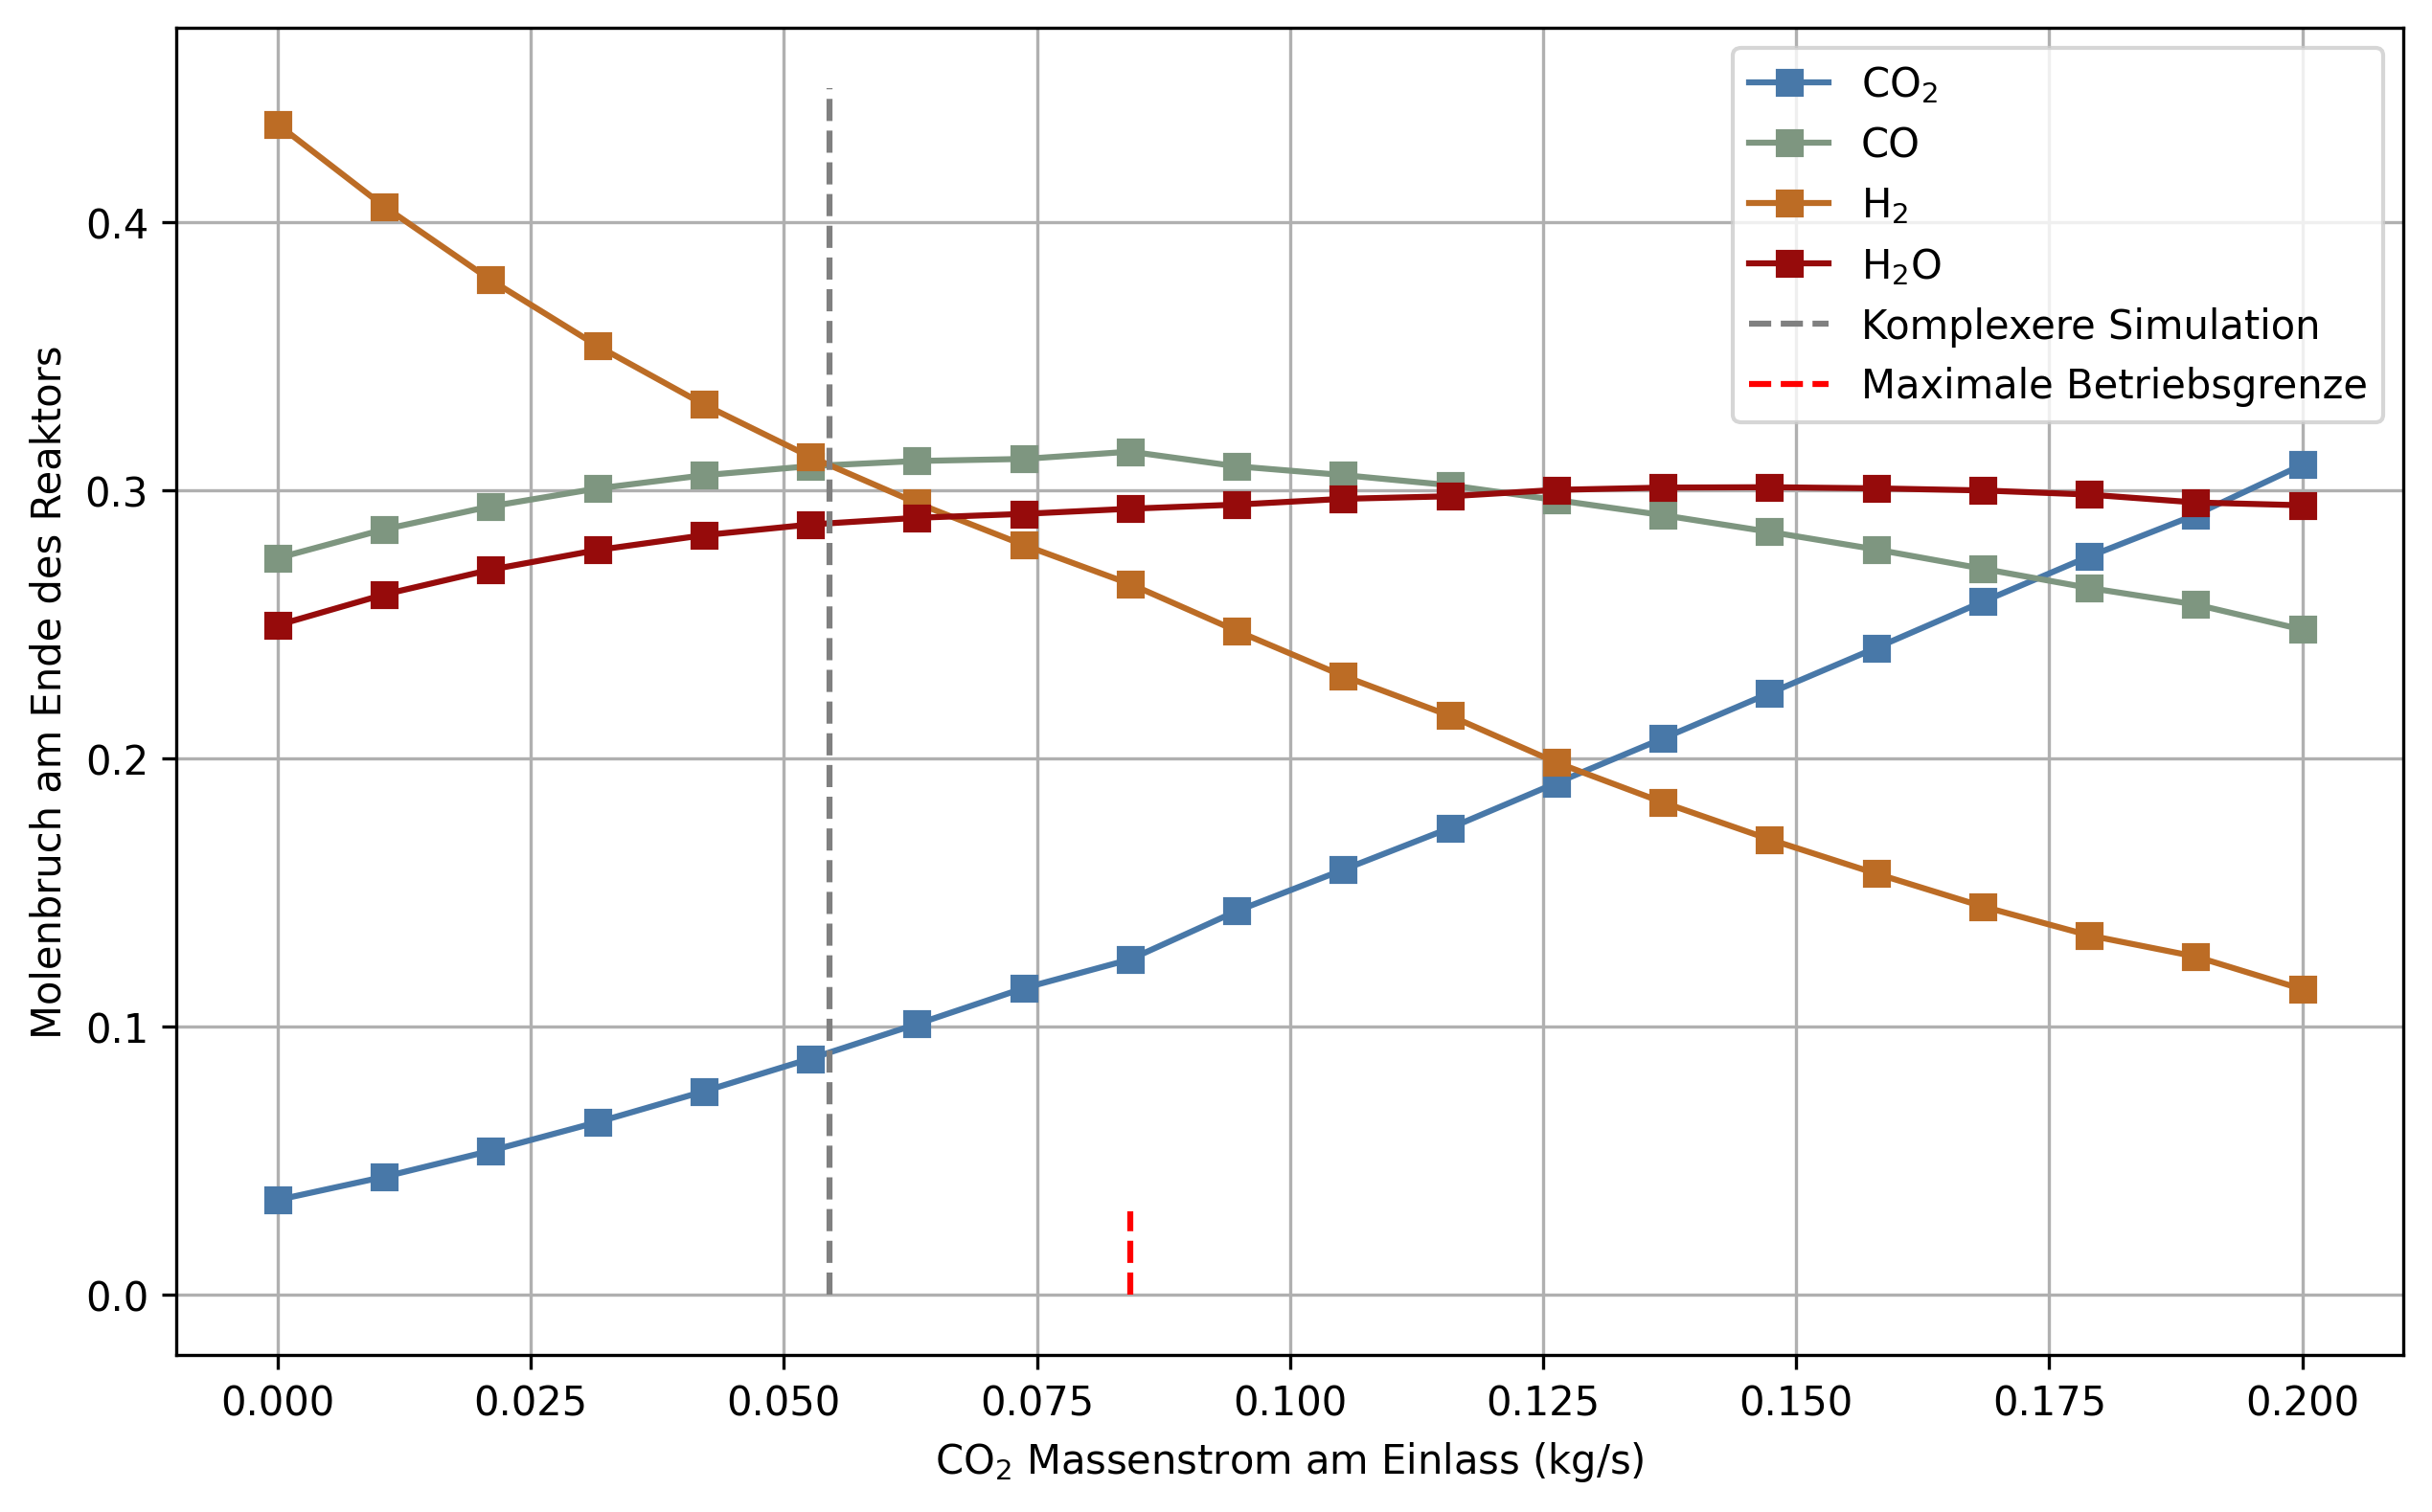
\includegraphics[width=0.9\linewidth]{img/Parameterstudie_CO2/Parameterstudie_CO2_Molenbruch_Ende.png}
        \caption{Simulierte maximale und minimale Temperatur im Reaktor (PFR)}
        \label{fig:parameterstudie_molenbruch}
    \end{figure}
    Während bei CO$_2$ freiem Betrieb Wasserstoff mit einem Molanteil von über 40\% vorliegt, sinkt dieser Wert mit steigender CO$_2$ Zufuhr deutlich. Gleichzeitig steigt der Stoffmengenanteil von CO anfangs leicht an, erreicht dann ein Plateau, bevor er bei hohen Strömen wieder abfällt. 

    Abbildung \ref{fig:parameterstudie_bilanz} verdeutlicht den Zusammenhang zwischen dem Verhältnis H$_2$/CO$_2$ am Reaktorausgang sowie der CO$_2$-Bilanz in Abhängigkeit vom eingespeisten CO$_2$-Massenstrom. 
    \begin{figure}[H]
        \centering
        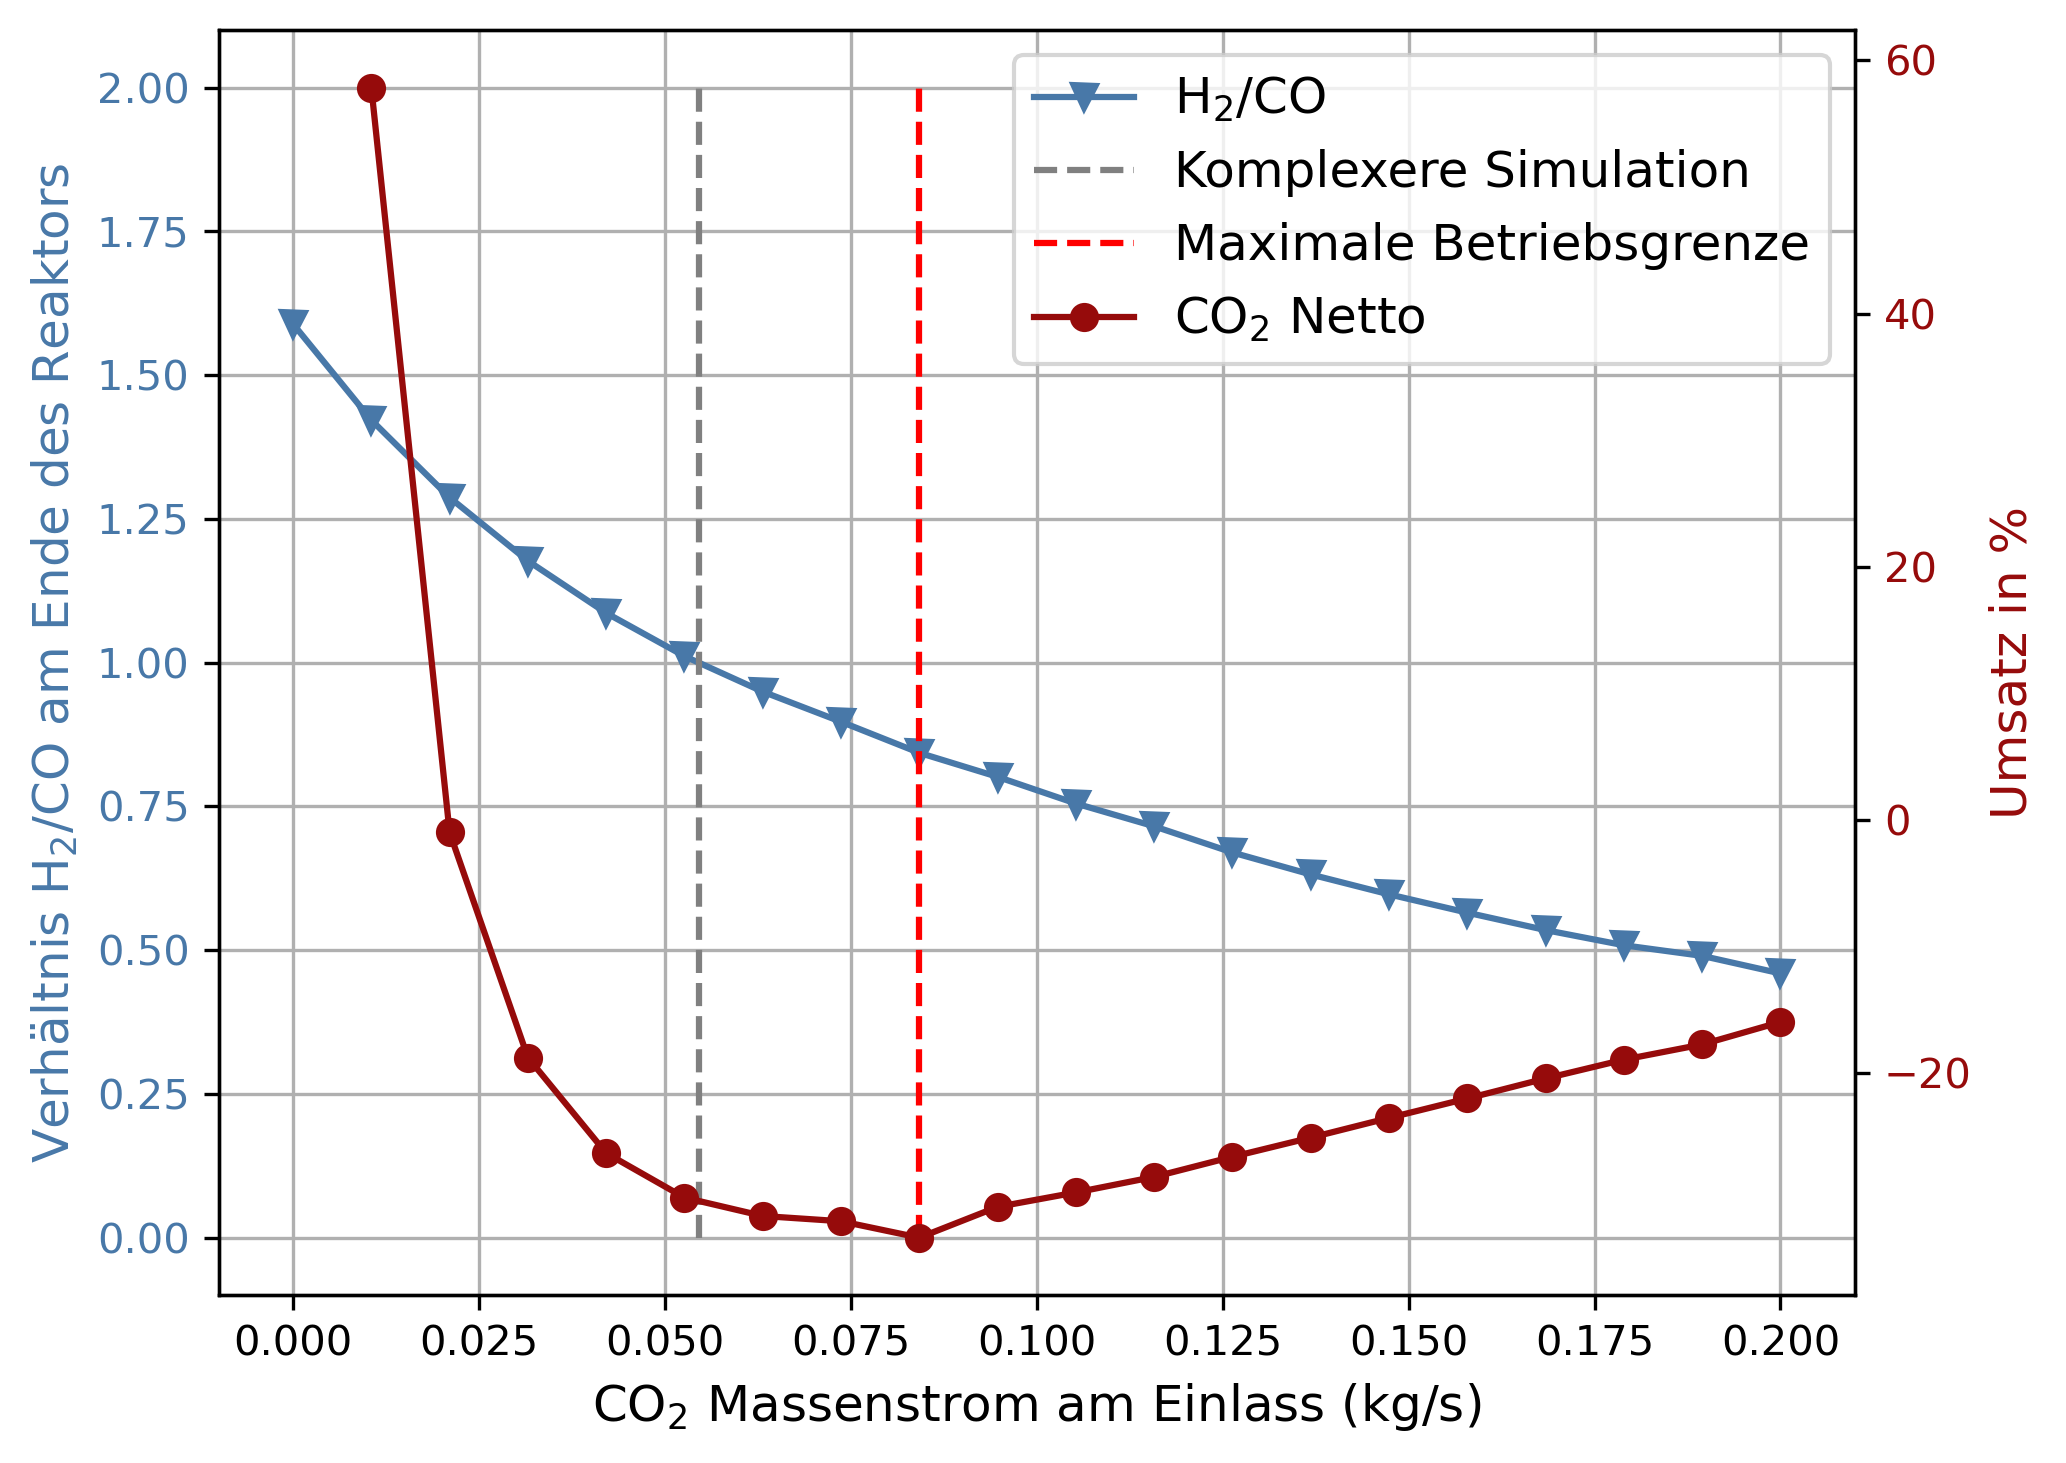
\includegraphics[width=0.9\linewidth]{img/Parameterstudie_CO2/Parameterstudie_CO2_Bilanz.png}
        \caption{Simulierte maximale und minimale Temperatur im Reaktor (PFR)}
        \label{fig:parameterstudie_bilanz}
    \end{figure}
    Mit steigender CO$_2$-Zufuhr sinkt das Verhältnis H$_2$/CO$_2$ stark ab. Während im CO$_2$-freien Betrieb noch Werte von über 12 erreicht werden, fällt das Verhältnis selbst bei moderater CO$_2$ Zufuhr stark ab und erreicht bei hohen Feedraten einen Wert von etwa 1. Damit zeigt sich, dass eine Zugabe von CO$_2$ die Wasserstoffdominanz im Produktgas deutlich reduziert. xxxxxxxxxxxxxxxxx % Hier nochmal als Quelle einfügen, wie Syngaszusammensetzung ist!

    Die CO$_2$-Bilanz, definiert als $\dot m_{CO_{2,aus}}-\dot m_{CO_{2,ein}}$, verdeutlicht die Netto-Bildung bzw. den Netto-Verbrauch von Kohlenstoffdioxid im Reaktor. Ohne CO$_2$-Feed ist die Bilanz positiv, da im Reaktor durch Oxidationsreaktionen (v.a. Gleichung \ref{eq:vollst_oxidation}) Kohlenstoffdioxid gebildet wird. Mit zunehmendem CO$_2$-Feed verschiebt sich die Bilanz zunehmend in den negativen Bereich. Bei hohen Feedströmen an Kohlenstoffdioxid wird findet somit eine höhere Bindung von CO$_2$ im Reaktor statt.

    Insgesamt ergibt sich, dass steigende CO$_2$ Zufuhren zwar zu einer deutlichen Absenkung des H$_2$/CO$_2$-Verhältnisses führen, gleichzeitig aber auch eine zunehmende chemische Nutzung von CO$_2$ im Reaktor erfolgt. 
    \section{Zusammenfassung}
    Die durchgeführte Parameterstudie verdeutlicht den erheblichen Einfluss einer CO$_2$-Zufuhr auf das Verhalten des betrachteten Reaktors. Bereits aus den Temperaturverläufen lässt sich erkennen, dass mit zunehmendem CO$_2$-Feedstrom sowohl die maximale als auch die minimale Reaktionstemperatur deutlich sinken. Verantwortlich dafür sind die hohe Wärmekapazität von CO$_2$ und die dadurch auftretenden Verdünnungseffekte. 

    Besonders großen Einfluss hat dieser Effekt auf die Bildung von Wasserstoff. Während dieser bei niedriger CO$_2$-Zugabe vergleichsweise viel gebildet wurde, sinkt die Bildung bei erhöhtem Feed deutlich. 

    Die CO$_2$-Bilanz liefert zudem wichtige Erkenntnisse. Ohne CO$_2$-Zugabe ist die Bilanz leicht positiv, was einen Nettoausstoß von CO$_2$ bedeutet. Mit zunehmendem CO$_2$-Massenstrom wird die Bilanz jedoch negativ, was bedeutet, dass mehr CO$_2$ verbraucht als emittiert wird. Dieser Nettoverbrauch steigt mit wachsendem Feed weiter an und belegt die zunehmende Bedeutung der CO$_2$-Reformierung sowie der Wassergas-Shift-Reaktion. Es ist erkennbar, dass der komplexere Fall mit CO$_2$ Zugabe zu einer negativen CO$_2$-Bilanz führt, netto also CO$_2$ verbraucht, anstatt zu produzieren. 
\fi 
%------------ neue Variante (Auswertung Extra) -------------------
    \section{Motivation}
        Um aus der herkömmlichen und industriell weit verbreiteten Partialoxidation einen Prozess weiterzuentwickeln, ist es wichtig, den Einfluss von Kohlenstoffdioxid im Feedstrom zu untersuchen. Eine gezielte Zugabe von CO$_2$ kann sowohl die Temperaturverteilung als auch die Kinetik im Reaktor maßgeblich beeinflussen und hat somit großen Einfluss auf die Zusammensetzung des Synthesegases. 

        Ziel der Parameterstudie ist es daher, den Effekt variierender CO$_2$-Feedraten auf Reaktionstemperaturen und Produktzusammensetzungen systematisch zu untersuchen. Besonders entscheidend für die Einschätzung des Prozesses und den Nutzen des Synthesegases ist dabei das Verhältnis H$_2$/CO sowie die CO$_2$-Bilanz des Prozesses. 
    \section{Methodik der Simulation}
        Für eine effiziente Parameterstudie wurde diese auf Basis des in Abbildung \ref{fig:reaktornetzwerk1} dargestellten Reaktornetzwerkmodells (ROM) durchgeführt. Das Modell basiert dabei auf der Annahme, dass im Reaktor eine vollständig durchmischte Flammzone (PSR) und eine Nachbrennzone (PFR) vorhanden sind. Ein lineares ROM ohne Rückkopplung führt dabei zu einer effizienten Berechnung, was komplexe Parameterstudien ermöglicht. 

        Die Simulationen wurden unter stationären Bedingungen mit der Software \textit{Chemkin-Pro} durchgeführt. Als Reaktionsmechanismus kam der in der Literatur als sehr gut beschriebene AramcoMech~2.0 zum Einsatz. 
        
        Der Massenstrom von CO$_2$ am Reaktoreintritt wurde dabei schrittweise zwischen 0~kg/s und 0,2~kg/s (entspricht 720 kg/h) variiert, während alle anderen Prozessparameter konstant gehalten wurden. Insgesamt wurden 20 Simulationen mit einer linearen Schrittweite des CO$_2$-Massenstroms durchgeführt. Für jede Simulation wurden die Temperatur- und Stoffmengenprofile der relevanten Spezies entlang der Nachbrennzone und die CO$_2$-Bilanz am Reaktorausgang überprüft.
    \section{Theoretische Erwartungen}
        Aufgrund thermodynamischer Eigenschaften und Reaktionsmechanismen des Systems lassen sich mehrere Effekte durch die Zugabe von CO$_2$ vorhersagen. 

        Da CO$_2$ eine hohe Wärmekapazität aufweist \cite{NIST_CO2_WebBook_General} und teilweise eine Verdünnung verursacht, ist bei steigendem Massenstrom CO$_2$ mit einer absinkenden Temperatur zu rechnen. Gleichzeitig fördert eine hohe Konzentration von CO$_2$ die stark endotherme Dry-Reforming-Reaktion (vgl. Gl. \ref{eq:dampfreformierung}). Diese Reaktion trägt somit zusätzlich zu einem Absinken der Temperatur bei.

        Die erhöhte CO$_2$-Konzentration führt zudem zu einer Verschiebung der Gleichgewichtslage der Wassergas-Shift-Reaktion (siehe Gl. \ref{eq:wassergas_shift}) hin zur Bildung von CO. Gleichzeitig sorgt die geringere Temperatur allerdings auch für eine Verschiebung in gegensätzliche Richtung. 

        Es ist damit zu rechnen, dass bei geringen CO$_2$-Mengen im Feed die Bildung von diesem überwiegt, während bei höheren Mengen im Feed eine Umsetzung von CO$_2$ in CO denkbar ist. Daraus ergibt sich, dass die CO$_2$-Bilanz bei hohen Massenströmen negativ wird. 
        
    \chapter{Aufbau eines reduzierten Reaktormodells}
    Ziel der Konstruktion eines reduzierten Reaktormodells (Reduced-Order-Model, ROM) ist es, durch Kombination mehrerer idealer Reaktoren ein Reaktornetzwerk aufzubauen, das eine möglichst genaue Modellierung des Reaktors ermöglicht. Dabei werden Strömungserscheinungen wie Bypass, Rezirkulation oder Reformierungszone. durch einzelne Reaktoren abgebildet. 
\iffalse
    \section{Rahmenbedingungen}
        Grundlage der Simulation ist ein Reaktor, an dem bereits experimentell zwei Versuche durchgeführt wurden, bei denen die Temperaturen und Stoffströme am Reaktorausgang ermittelt wurden. Die Rahmenbedingungen beider Versuche sind in Tabelle \ref{tab:rahmenbedingungen_versuche} dargestellt.
        \begin{table}[H]
            \centering
            \caption{Vergleich der Prozessfälle \cite{gonzales}}
            \begin{tabular}{llll}
            \toprule
            \textbf{Variablen} & & \textbf{Fall 1} & \textbf{Fall 2} \\
            \midrule
            \textbf{1. Erdgas} & Temperatur [°C] & 66,6 & 67,5 \\
                               & Massenstrom [kg/h] & 182,4 & 153,3 \\
            \midrule
            \textbf{2. Kohlendioxid} & Temperatur [°C] & -- & 67,5 \\
                                     & Massenstrom [kg/h] & 0 & 196,4 \\
            \midrule
            \textbf{3. Sauerstoff} & Temperatur [°C] & 231,9 & 231,2 \\
                                   & Massenstrom [kg/h] & 252,2 & 246,9 \\
            \midrule
            \textbf{4. Dampf} & Temperatur [°C] & 353,4 & 353,4 \\
                              & Massenstrom [kg/h] & 38,7 & 39,4 \\
            \midrule
            Wandwärmeverlust [kW] & & 30 & 30 \\
            Reaktorvolumen [L] & & 134 & 134 \\
            \midrule
            \textbf{Kommentar} & & Referenz & CO\textsubscript{2}-Zugabe \\
            \bottomrule
            \end{tabular}
            \label{tab:rahmenbedingungen_versuche}
        \end{table}
        Neben den Werten des Feedstroms sind zusätzlich die Geometrien des Reaktors und des Brenners bekannt, die in Abbildung \ref{fig:reaktorgeometrie} dargestellt sind. 
        \begin{figure}[H]
            \centering
            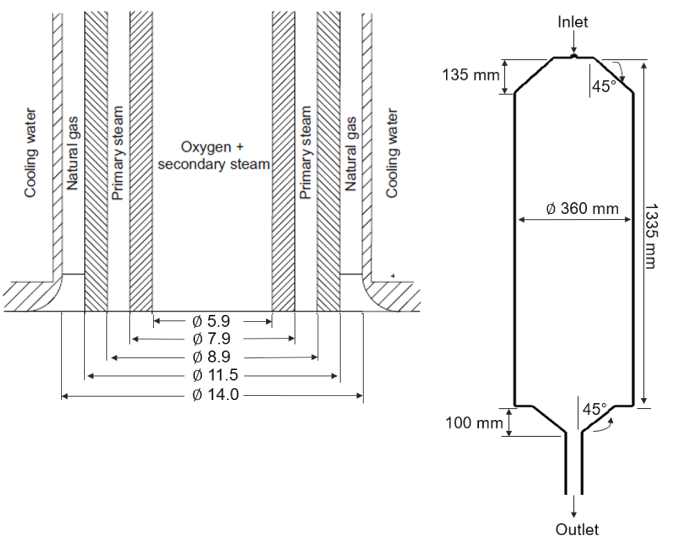
\includegraphics[width=0.8\linewidth]{img/sonstiges/Reaktorgeometrien.png}
            \caption{Geometrien des Reaktors sowie des Brenners}
            \label{fig:reaktorgeometrie}
        \end{figure}
    \section{Vorbetrachtungen}
        Zur Vorbetrachtung liegt bereits eine CFD-Analyse sowie ein komplexes ROM-Modell vor. 
        \begin{figure}[H]
            \centering
            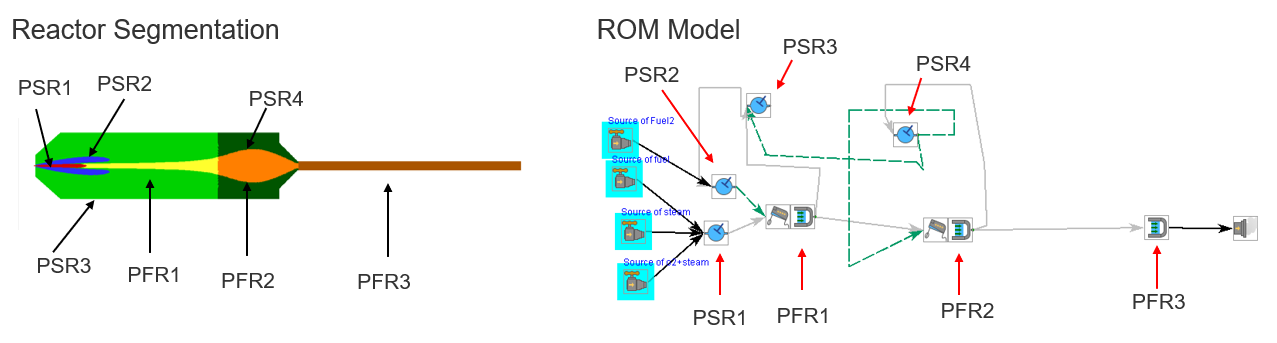
\includegraphics[width=1\linewidth]{img/sonstiges/Reactor Segmentation.png}
            \caption{Reaktorsegmentierung und komplexes ROM auf basis einer CFD-Simulation \cite{gonzales}}
            \label{fig:reaktorsegmentierung}
        \end{figure}
        Um den Einfluss der einzelnen Reaktoren auf die Simulationsergebnisse zu ermitteln, wird das in Abschnitt \ref{sec:Simulationen_reaktionsmechanismus} dargestellte Reaktornetzwerk schrittweise erweitert. Nach jeder Erweiterung werden die Simulationsergebnisse mit den Experimentaldaten verglichen. 

        Durch diesen iterativen Ansatz lässt sich nicht nur die Relevanz einzelner Reaktoren für die Abbildung der experimentellen Daten bestimmen, sondern auch eine Grundlage für die spätere Modellvereinfachung schaffen. Auf diese Weise kann zwischen einer möglichst hohen Modellgenauigkeit und einer zugleich geringen Rechenkomplexität abgewogen werden. Zudem wird sichtbar, welche Teilreaktoren für die wesentlichen Stoff- und Energiebilanzen entscheidend sind und welche nur einen geringen Beitrag zur Gesamtvorhersage leisten. Damit wird eine systematische Basis geschaffen, um in späteren Schritten reduzierte Modelle (ROMs) abzuleiten, die für Prozessoptimierungen und Echtzeitanwendungen besser geeignet sind.
\fi 
    \section*{Entwicklung eines komplexen Reaktornetzwerks}
        \label{sec:erweiterung_rom}
        Im Folgenden werden die einzelnen Entwicklungsschritte eines einfachen Modells, wie es bereits beschrieben wurde, bis zu einem komplexen Netzwerk einzeln aufgeführt. Dabei sind die Reaktoren, welche die Flamm- sowie Bypasszone darstellen, orange gefärbt, während die Reaktoren der Reformierungszone blau dargestellt sind. Die ab Reaktornetzwerk 3 verwendete Rezirkulationszone bzw. die Rezirkulationszonen sind zusätzlich grün dargestellt.
        \subsection*{Reaktornetzwerk 1}
            Abbildung \ref{fig:reaktornetzwerk1} zeigt die einfachste Form des untersuchten Reaktornetzwerks, bestehend aus einem PSR und einem nachgeschalteten PFR. In diesem Aufbau wird zunächst die schnelle chemische Umsetzung im PSR angenommen, der durch vollständige Durchmischung charakterisiert ist. Anschließend erfolgt im PFR eine strömungsdominierte Nachreaktion, in der axiale Temperatur- und Konzentrationsverläufe berücksichtigt werden. Der Wärmeverlust erfolgt ausschließlich über den PFR.

            Dieses zweistufige Modell ist die Grundlage für alle folgenden Erweiterungen und ermöglicht eine erste Beschreibung der Hauptreaktionen während der partiellen Oxidation.
            \begin{figure}[H]
                \centering
                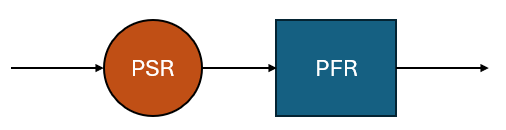
\includegraphics[width=0.7\linewidth]{img/Erweiterungen/1.png}
                \caption{Schematische Darstellung des ersten Reaktornetzwerks, bestehend aus einer Flammzone (orange) und einer Nachbrennzone (blau)}
                \label{fig:reaktornetzwerk1}
            \end{figure}
            Dabei hat der PSR ein Volumen von 13,7~Litern, während der PFR ein Volumen von ca. 116~Litern aufweist. Insgesamt ergibt sich so das in Tabelle \ref{tab:rahmenbedingungen_versuche} beschriebene Volumen von 130 Litern. Der Wärmeverlust wird vollständig durch den PFR abgebildet und beträgt 30~kW. 
        \subsection*{Reaktornetzwerk 2}
            Im nächsten Schritt (Abbildung \ref{fig:reaktornetzwerk2}) wird das System um einen zweiten PSR erweitert, der die Einspeisung eines zweiten Stoffstroms parallel zur Flammzone ermöglicht. 

            Diese Konfiguration dient der realitätsnäheren Beschreibung des Zulaufs, da ein Teil des eingebrachten Erdgases an der Flammzone vorbeiströmt (Bypass). Durch diese Erweiterung liegt am PFR-Eintritt eine veränderte Gaszusammensetzung vor. In diesem PSR befindet sich ausschließlich Erdgas, da dieses als äußeres Feedgas (siehe Abbildung \ref{fig:reaktorgeometrie}) zugeführt wird. Im Vergleich zum vorhergehenden Reaktornetzwerk wurde der Erdgasstrom zu gleichen Verhältnissen aufgeteilt, die sonstigen Stoffströme verlaufen vollständig durch den PSR, der die Flammzone darstellt.  
            \begin{figure}[H]
                \centering
                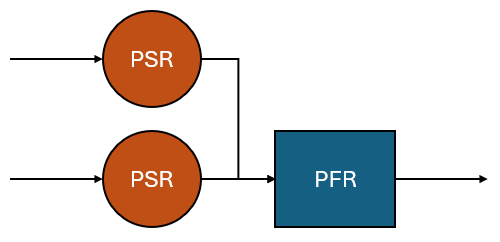
\includegraphics[width=0.7\linewidth]{img/Erweiterungen/2.png}
                \caption{Schematische Darstellung des zweiten Reaktornetzwerks, bestehend aus Flammzone mit Bypass (orange) und einer Nachbrennzone (blau)}
                \label{fig:reaktornetzwerk2}
            \end{figure}
        \subsection*{Reaktornetzwerk 3}
            Das Reaktornetzwerk 2 wird um eine Rezirkulationszone erweitert. Um einen Stoffaustausch zwischen dem PFR und der Rezirkulationszone zu ermöglichen, wird der PFR in mehrere PFRs unterteilt. In diesem vereinfachten Modell wird davon ausgegangen, dass die Rezirkulationszone nur im Austausch mit dem Ende des Reaktors und der Bypass Zone steht. Es wird ein zusätzlicher PFR als Reaktorausgang hinzugefügt. Im Bereich des ersten PFRs tritt kein Wärmeverluststrom auf, da dieser am PSR, der die Rezirkulationszone darstellt, simuliert wird. Der Gesamtwärmeverluststrom ergibt sich insgesamt aus dem Wärmeverluststrom des PSRs der Rezirkulationszone (20~kW) und dem Wärmeverluststrom des zweiten PFRs (10~kW). 

            Das Rezirkulationsverhältnis wurde auf 0,95 festgelegt. Damit wird ein sehr hoher Anteil des Abgasstroms aus der Nachbrennzone erneut in das Reaktorsystem zurückgeführt. Konkret bedeutet dies, dass 95~\% des aus der Nachbrennzone austretenden Massenstroms rezirkuliert und nur 5~\% als Produktstrom abgeführt werden. 
            \begin{figure}[H]
                \centering
                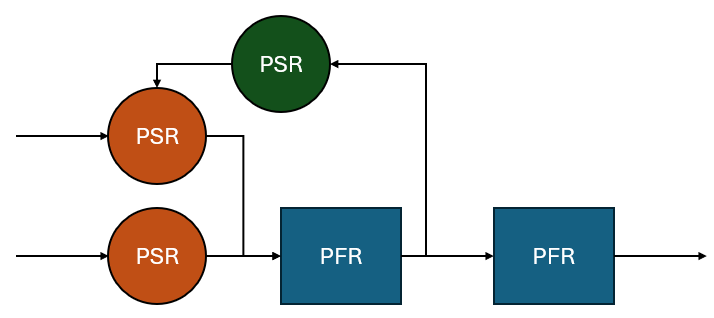
\includegraphics[width=0.8\linewidth]{img/Erweiterungen/3.png}
                \caption{Schematische Darstellung des dritten Reaktornetzwerks, bestehend aus Flammzone mit Bypass (orange), einer Nachbrennzone (blau) und einer Rezirkulationszone (grün)}
                \label{fig:reaktornetzwerk3}
            \end{figure}
            In diesem Modell ist der Durchmesser und die Länge des ersten PFRs sehr gering, weshalb die Rezirkulationszone einen großen Anteil am Volumen einnimmt. 
        \subsection*{Reaktornetzwerk 4}
            Im Vergleich zum vorherigen Reaktornetzwerk wurde ein Stoffstrom von der Mitte des ursprünglichen PFRs zur Rezirkulationszone hinzugefügt, sodass diese jetzt mit mehreren Reaktoren gekoppelt ist. Dies ist in Abbildung \ref{fig:reaktornetzwerk4} dargestellt. Dieses Rezirkulations\-verhältnis wurde analog zu Reaktornetzwerk 3 als 0,95 festgelegt. Die Wärmeverlustströme sind wie in Modell 3 definiert. 
            \begin{figure}[H]
                \centering
                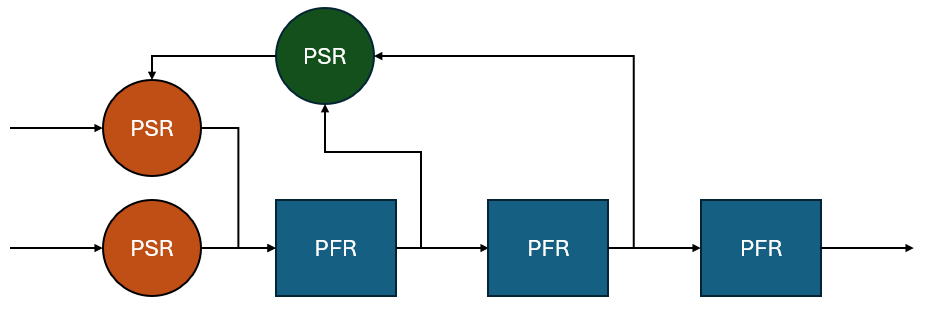
\includegraphics[width=0.8\linewidth]{img/Erweiterungen/4.png}
                \caption{Schematische Darstellung des vierten Reaktornetzwerks, bestehend aus Flammzone mit Bypass (orange), einer Nachbrennzone (blau) und einer Rezirkulationszone (grün)}
                \label{fig:reaktornetzwerk4}
            \end{figure}
        \subsection*{Reaktornetzwerk 5}
            Im finalen Schritt wird die Rezirkulationszone in zwei verschiedene Reaktoren unterteilt und es werden Stoffströme von beiden Reaktoren in der Rezirkulationszone zur Nachbrennzone berücksichtigt. Der linke PSR umfasst etwa 75~\% und der rechte PSR etwa 25~\% des ursprünglichen Volumens der Rezirkulationszone. Das Reaktornetzwerk ist in Abbildung \ref{fig:reaktornetzwerk5} dargestellt. Die Wärmeverluste der in Netzwerk 3 beschriebenen Rezirkulationszone werden abhängig von den Volumina auf beide PSRs aufgeteilt. Die Auftrennung der Stoffströme nach den Reaktoren der Rezirkulationszone entsprechen 0,5.
            \begin{figure}[H]
                \centering
                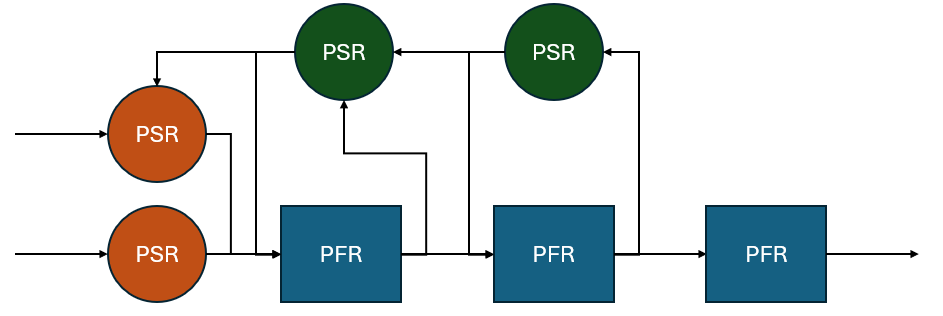
\includegraphics[width=0.8\linewidth]{img/Erweiterungen/5.png}
                \caption{Schematische Darstellung des fünften Reaktornetzwerks, bestehend aus Flammzone mit Bypass (orange), einer Nachbrennzone (blau) und einer Rezirkulationszone aus zwei PSRs (grün)}
                \label{fig:reaktornetzwerk5}
            \end{figure}
\iffalse
    \section{Auswertung}
        \iffalse
        Da sich in den oben beschriebenen Reaktionsmechanismen die Länge der PFRs unterscheidet, ist ein direkter Vergleich der Verläufe innerhalb dieser Reaktoren nicht umsetzbar. Vergleichbar sind jedoch einzelne Punkte im Reaktor sowie die Zusammensetzung und Temperatur des Gases am Outlet. In Abbildung \ref{fig:erweiterungen_messpunkte} ist dargestellt, um welche Messpunkte es sich handelt. 
        \begin{figure}[H]
            \centering
            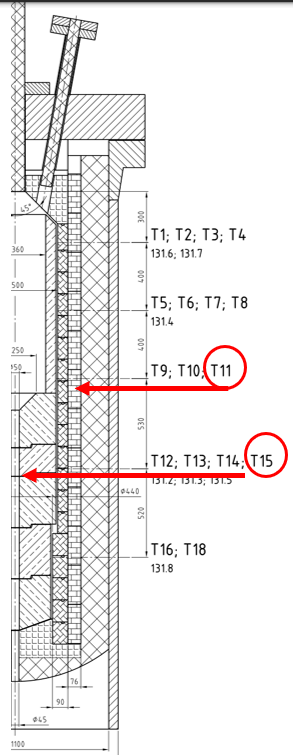
\includegraphics[width=0.2\linewidth]{img/Erweiterungen/Messpunkte.png}
            \caption{Messpunkte im Reaktor \cite{gonzales}}
            \label{fig:erweiterungen_messpunkte}
        \end{figure}
        \fi 

        Da sich in den oben beschriebenen Reaktionsmechanismen die Länge der PFRs unterscheidet, ist ein direkter Vergleich der Verläufe innerhalb dieser Reaktoren nicht umsetzbar. Vergleichbar sind allerdings die Zusammensetzungen der Gase am Outlet, zu denen auch Experimentelle Daten zum Vergleich vorliegen. In Abbildung \ref{fig:erweiterungen_vergleich_stoffe} sind die ermittelten Gaszusammensetzungen im Vergleich zu den Experimentell ermittelten Werten dargestellt. 
        \begin{figure}[H]
            \centering
            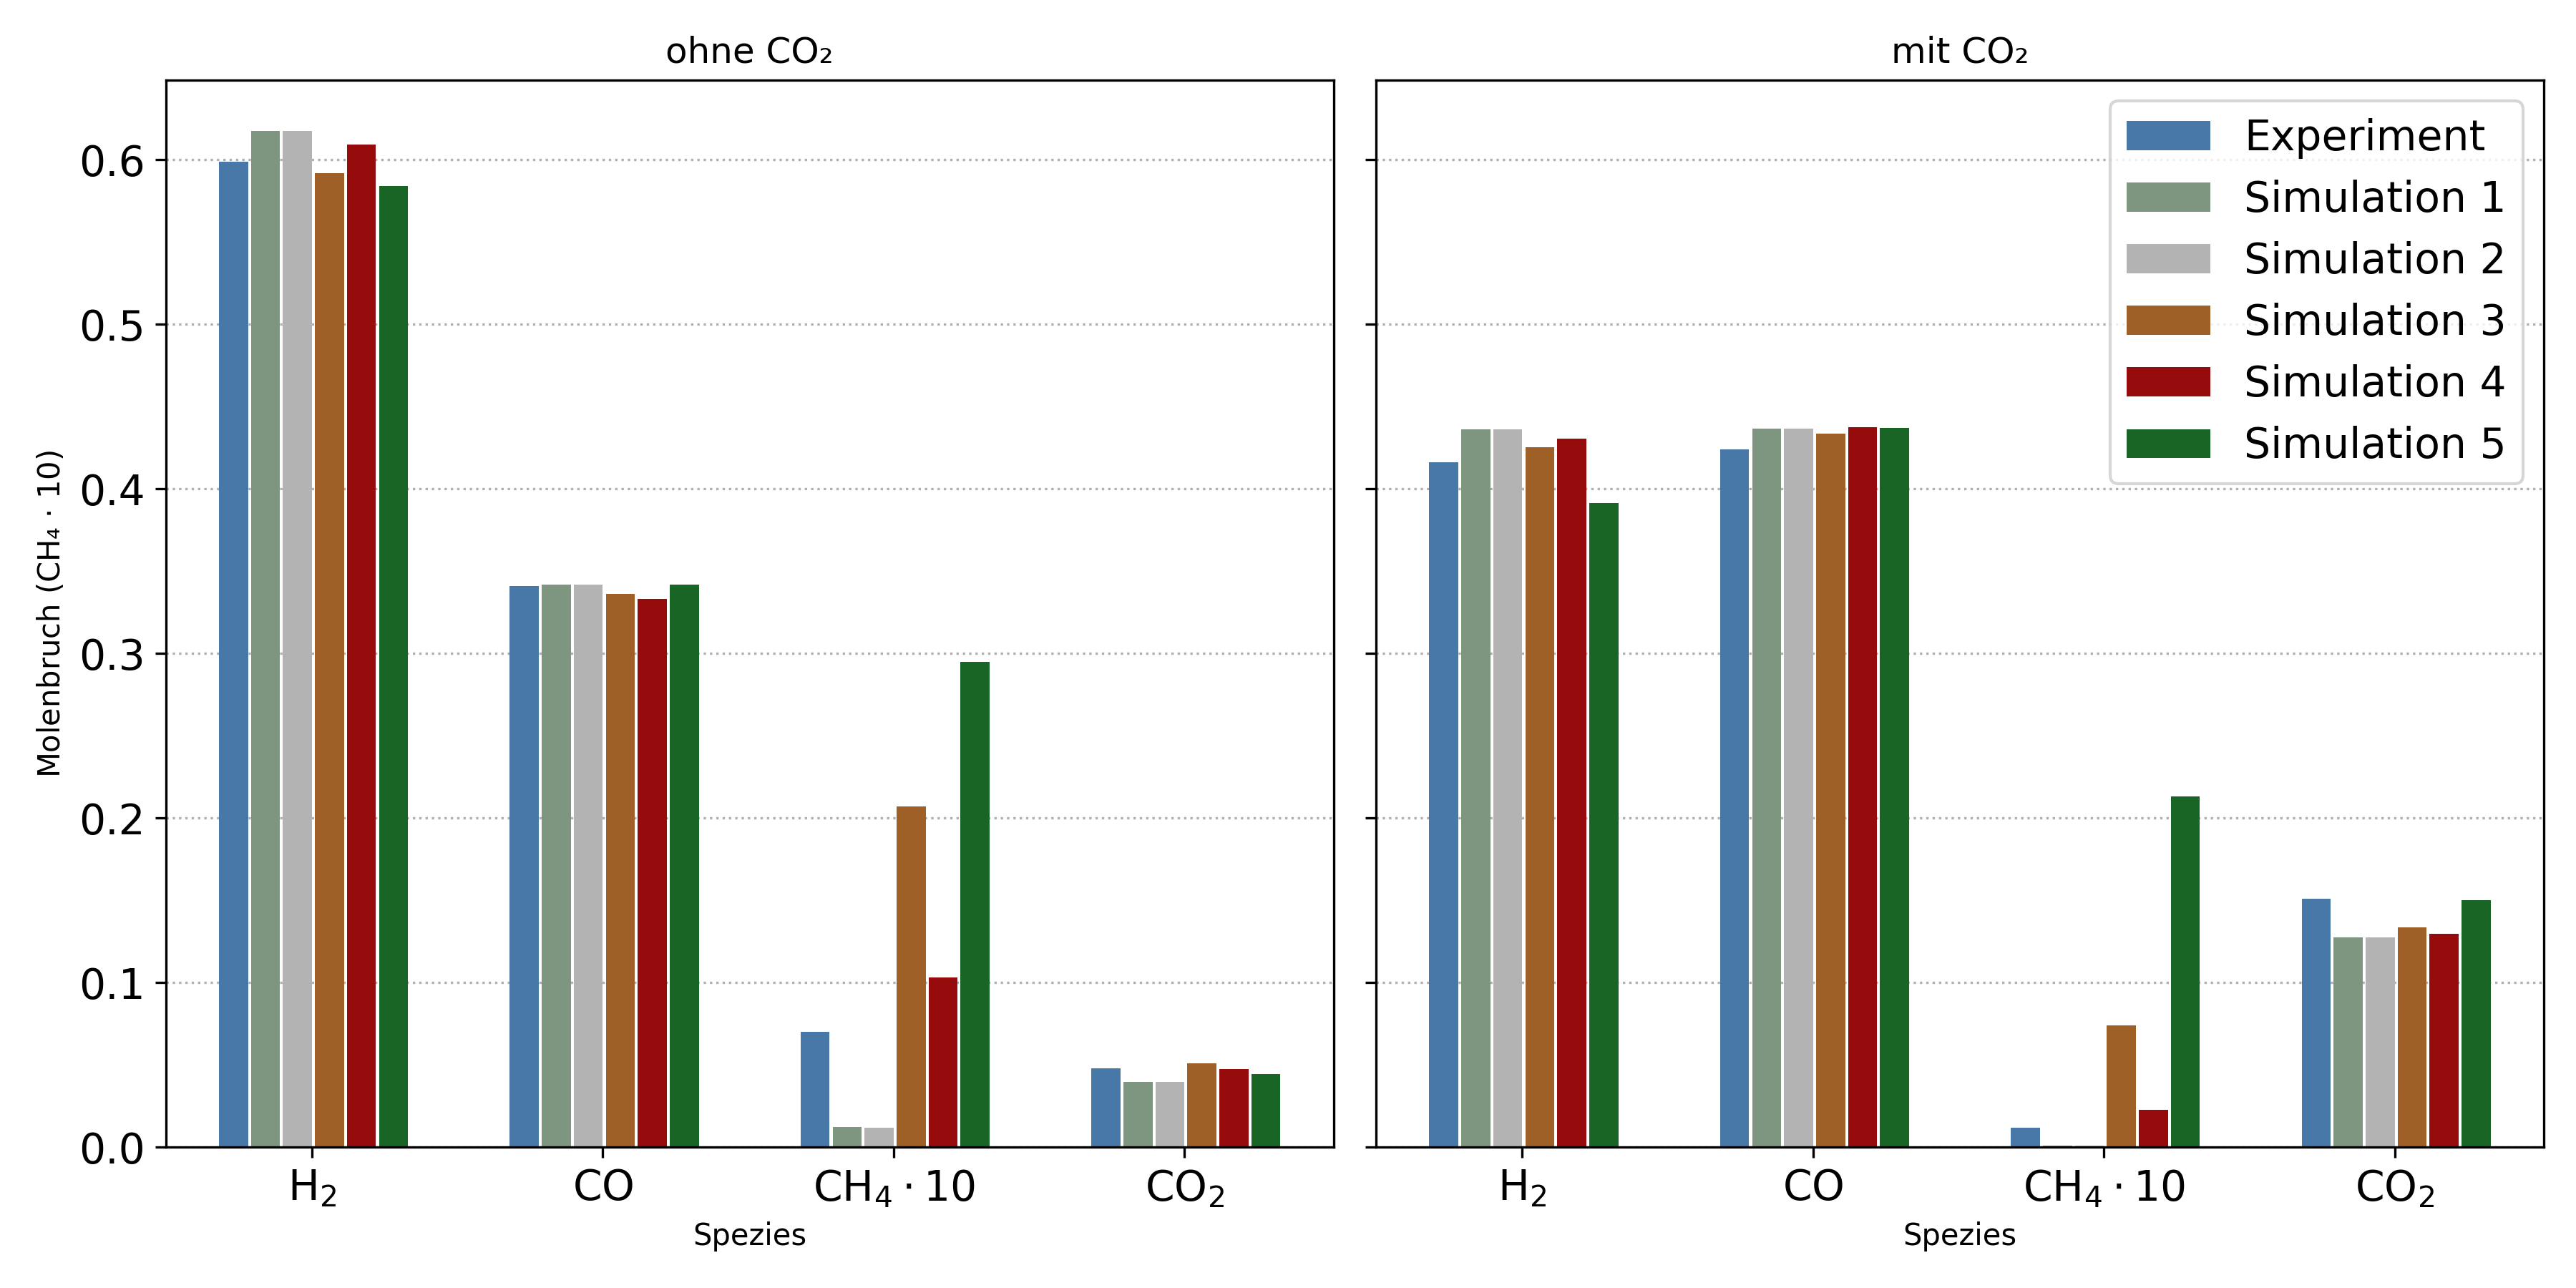
\includegraphics[width=0.9\linewidth]{img/Erweiterungen/Vergleich_Erweiterungen.png}
            \caption{Ergebnisse der Abgaszusammensetzungen und Vergleich mit den Werten der Experimente \cite{gonzales}}
            \label{fig:erweiterungen_vergleich_stoffe}
        \end{figure}
        Es ist erkennbar, dass die Größenordnungen aller Simulationen gleich sind. Dennoch gibt es Abweichungen zwischen den einzelnen Simulationen. Gerade der Schlupf von Methan (Methangehalt im Abgas) ist eine wichtige Kenngröße für diesen Prozess. Dabei kann man erkennen, dass die einfachsten Modelle einen deutlich zu niedrigen Methanschlupf haben, während die komplexen Modelle 3 und 5 einen deutlich zu hohen Schlupf von Methan aufweisen. Simulation 4 ist, wenn man nur den Schlupf von Methan betrachtet, die beste Simulation. 

        Zudem wurden in dem Reaktor durch zwei Thermoelemente Temperaturen gemessen, zusätzlich wurde die Austrittstemperatur als Vergleichswert bereits mit dem Programm AspenPlus bestimmt. Die Lage der Messpunkte in dem Reaktor sind in Abbildung \ref{fig:erweiterungen_messpunkte} zu erkennen. 
        \begin{figure}[H]
            \centering
            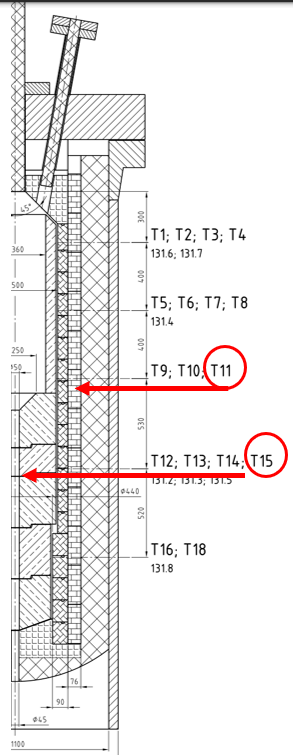
\includegraphics[width=0.2\linewidth]{img/Erweiterungen/Messpunkte.png}
            \caption{Messpunkte im Reaktor \cite{gonzales}}
            \label{fig:erweiterungen_messpunkte}
        \end{figure}
        Analog zu Abbildung \ref{fig:erweiterungen_vergleich_stoffe} können die Temperaturen an den verschiedenen Messpunkkten in Abbildung \ref{fig:erweiterungen_vergleich_temperaturen} dargestellt werden. 
        \begin{figure}[H]
            \centering
            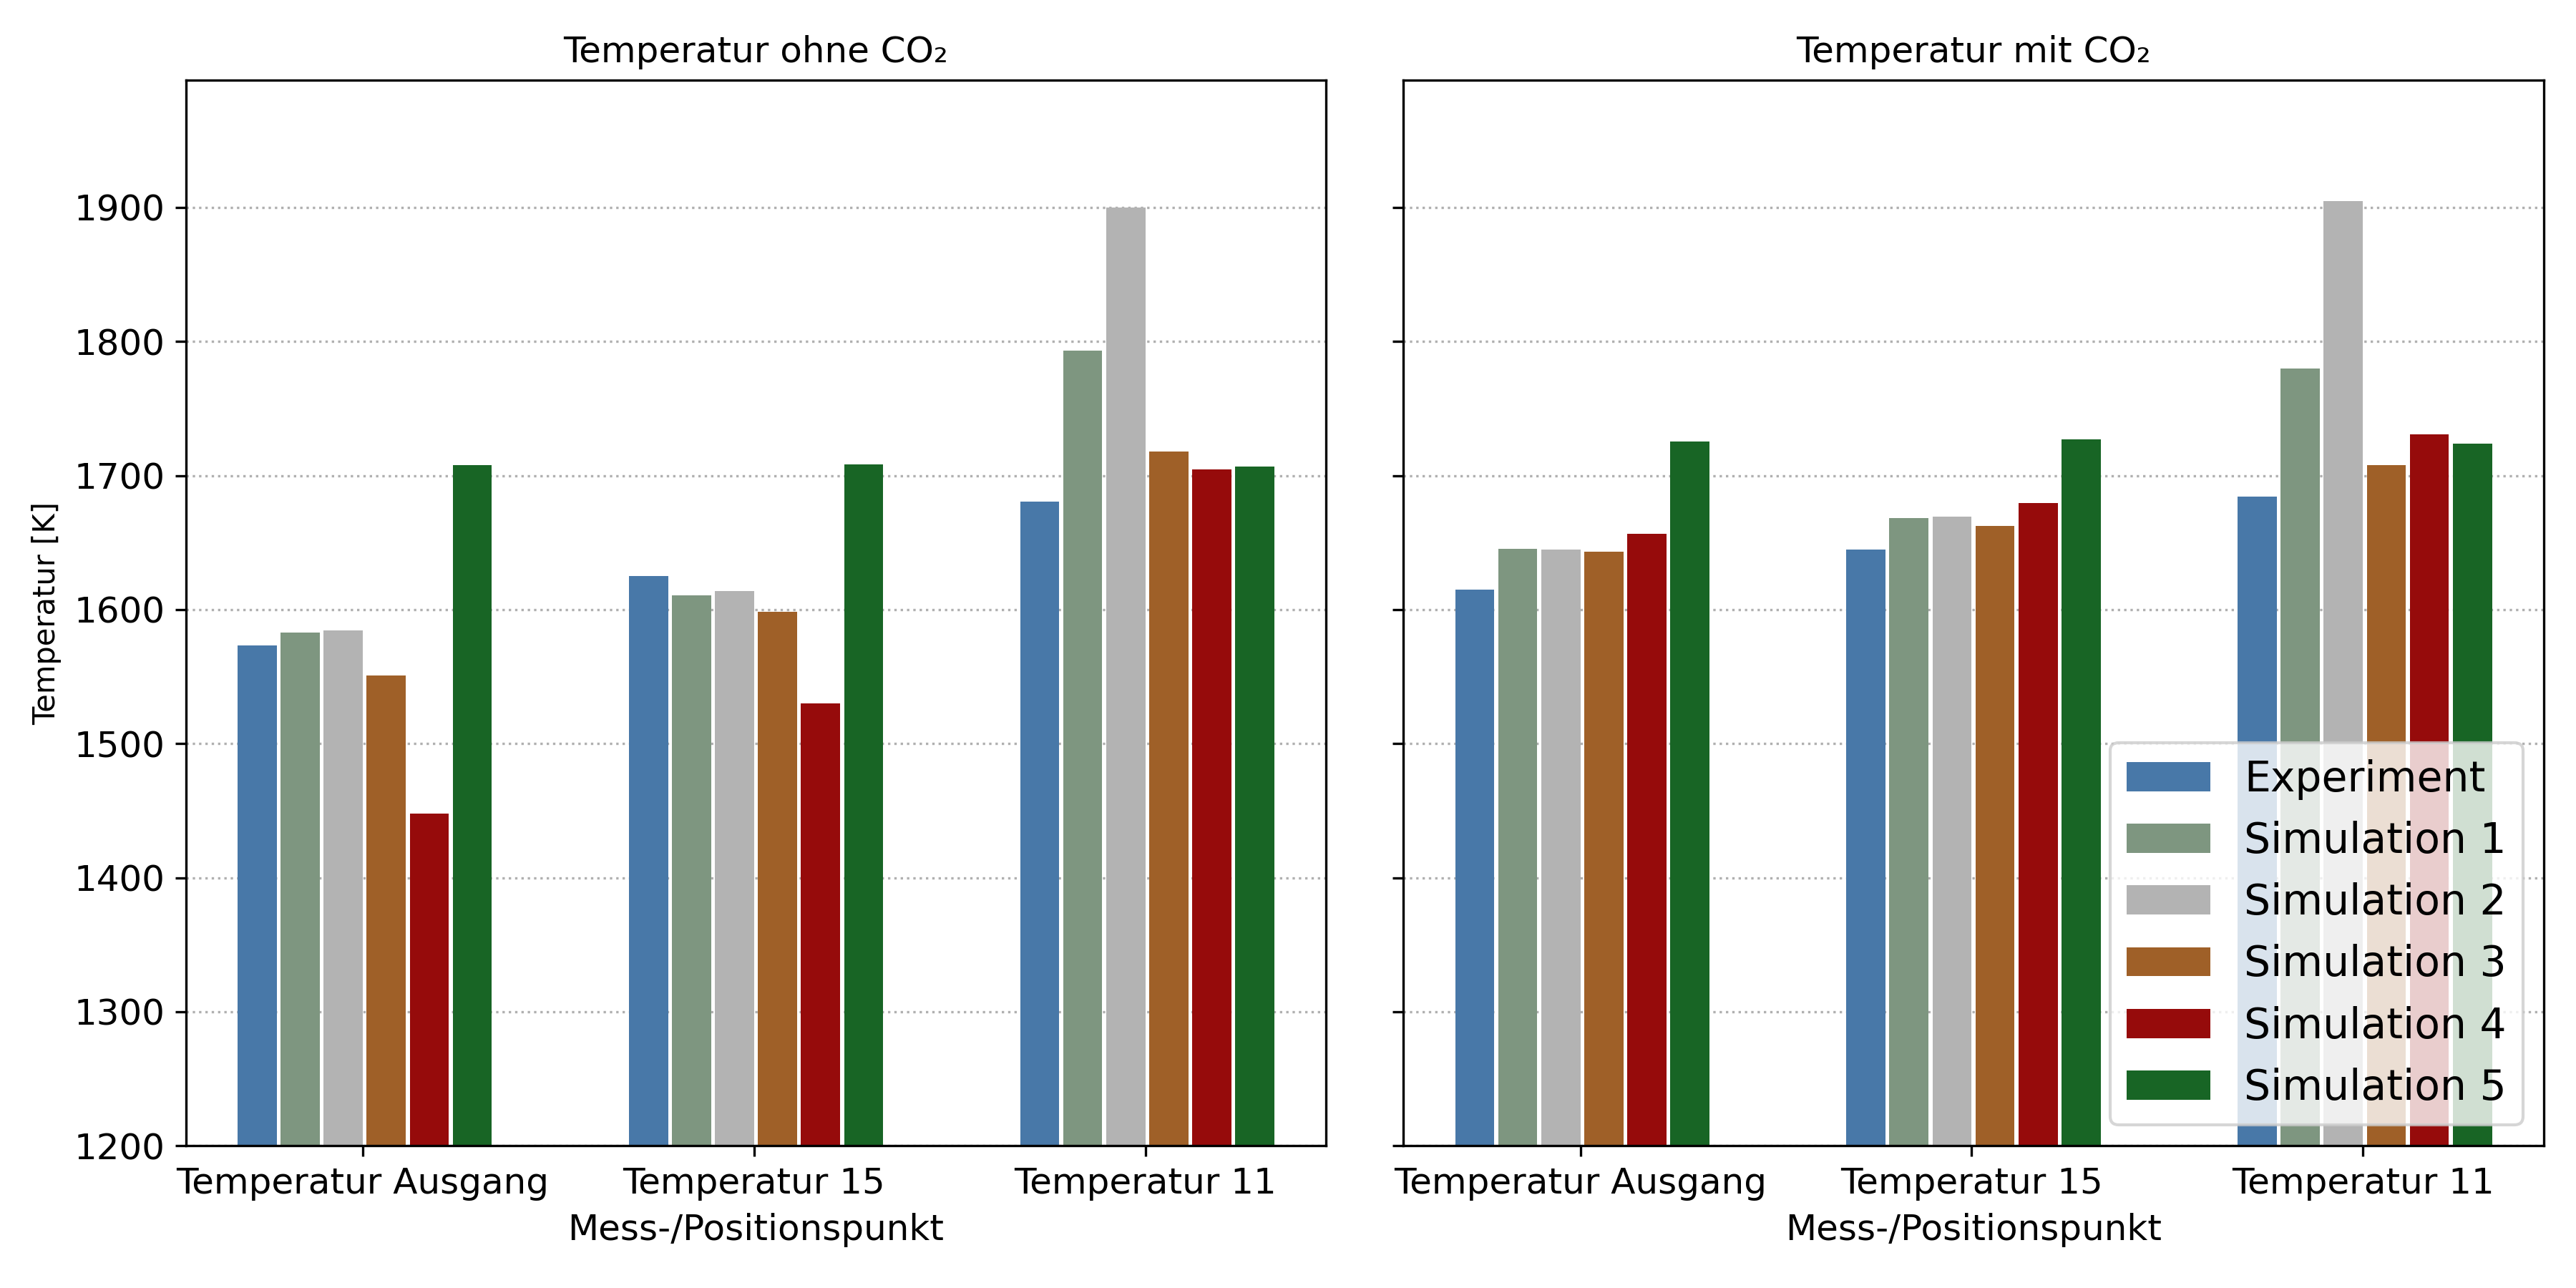
\includegraphics[width=0.9\linewidth]{img/Erweiterungen/Vergleich_Temperaturen.png}
            \caption{Ergebnisse der simulierten Temperaturen und Vergleich mit den gemessenen Temperaturen im Reaktor \cite{gonzales}}
            \label{fig:erweiterungen_vergleich_temperaturen}
        \end{figure}
        Wie auch bei den Stoffmengen liegen die Temperaturen größtenteils in einem ähnlichen Temperaturbereich. Es ist jedoch erkennbar, dass die Temperaturen der komplexesten Simulation allerdings deutlich zu hoch sind. Auch kann man eine deutlich zu geringe Temperatur des einfachsten Modells erkennen, die nur bei einer Zugabe von CO$_2$ auftritt, jedoch nicht ohne diese. 

        Zur quantitativen Bewertung der Modellgüte wurde ein relativer Fehlerwert eingesetzt. Für jede simulierte Größe wird der relative Fehler berechnet:
        \begin{align}
            E = \frac{\vert x_{sim} - x_{exp}\vert}{x_{exp}} 
        \end{align}
        Anschließend wird der Mittelwert über alle Größen gemittelt, sodass ein dimensionsloser Kennwert für jede Simulation entsteht. Dieser Wert ist direkt als mittlere prozentuale Abweichung intepretierbar, ein kleinerer Wert bedeutet eine höhere Übereinstimmung der Daten. 

        In Tabelle \ref{tab:relativer_fehler_vergleich} sind die Ergebnisse dieser Analyse aufgeführt. 
        \begin{table}[H]
            \centering
            \begin{tabular}{lcc}
                \toprule
                \textbf{Modell} & \textbf{Versuch 1} & \textbf{Versuch 2} \\
                \midrule
                1 & 0,159 & 0,261 \\
                2 & 0,169 & 0,190 \\
                3 & 0,300 & 0,765 \\
                4 & \textbf{0,096} & \textbf{0,167} \\
                5 & 0,494 & 2,426 \\
                \bottomrule
            \end{tabular}
            \caption{Bewertung der Modelle anhand des mittleren relativen Fehlers (MRE). Ein Wert von 0 entspricht perfekter Übereinstimmung, höhere Werte bedeuten größere Abweichungen.}
            \label{tab:relativer_fehler_vergleich}
        \end{table}
        In beiden Fällen weist Modell 4 die geringste Abweichung zu den experimentaldaten auf und kann somit als bestes Modell betrachtet werden. Im ersten Fall (ohne zusätzliches CO$_2$ im Feed) liegen alle Werte in einem moderatem Bereich, wobei insbesondere die einfachen Modelle 1 und 2 ebenfalls eine gute Genauigkeit vorweisen. 


        Im zweiten Fall (mit Zugabe von CO$_2$) verschlechtern sich alle Werte deutlich. Dies ist sowohl durch die erhöhte Komplexität der Reaktionschemie durch CO$_2$ (z.B. Dry Reforming und Wassergas-Shift-Reaktion) als auch auf die verstärkte Bedeutung kleiner Restkonzentrationen zurückzuführen, bei denen bereits kleine Mengen zu hohen relativen Fehlern führen. Besonders deutlich wird das am Modell 5, dessen MRE-Wert mehr als eine Größenordnung über den besten Modellen liegt.

        Auch ist in Modell 2 besonders auffällig, dass die Temperaturen deutlich unter allen anderen liegen. Dies kann nicht durch die nicht vorhandene Reaktion von Erdgas durch den Bypass erklärt werden, da dieses Modell ein viel zu geringen Schlupf von Methan aufweist. \alert{Vielmehr muss der Bypass ohne Rezirkulationszone zu einer Verschiebung der Gleichgewichtslagen in der Reformierungszone sorgen, wodurch die endothermen Reaktionen stark begünstigt werden.}

        Zusammenfassend lässt sich feststellen, dass die Modelle die Betriebsweisen ohne zusätzliches CO$_2$ als Feed besser modelliert werden können. Gleichzeitig bestätigt die Auswertung, dass ROM 4 in beiden Fällen die besten Ergebnisse liefert. 
\fi
    
\chapter{Ergebnisse und Diskussion}
     Im Rahmen dieser Studienarbeit wurden verschiedene Parameterstudien zur Modellierung der nichtkatalytischen Partialoxidation (POx) von Erdgas durchgeführt und hinsichtlich verschiedener Eigenschaften miteinander zu verglichen. 
     \section{Wahl des Reaktionsmechanismus}
        \label{sec:auswertung_mechanismus}
        Wie in Kapitel \ref{sec:reaktionsmechanismen_literatur} beschrieben, wurden die in dieser Studienarbeit eingesetzten Reaktionsmechanismen nicht speziell für die partielle Oxidation, sondern für Verbrennungsprozesse von Kohlenwasserstoffen entwickelt. Deshalb besteht die Notwendigkeit einer Validierung und eines Vergleichs der eingesetzten Mechanismen.
        Da alle Simulationen der verschiedenen Reaktionsmechanismen in einem identischen Reaktornetzwerk unter konstanten Bedingungen durchgeführt wurden, ist ein Vergleich der Gaszusammensetzungen am Reaktorausgang möglich. In Abbildung \ref{fig:auswertung_vergleich_exp_stoffe} sind diese Zusammensetzungen für beide simulierten Fälle dargestellt. Zur verbesserten Darstellung wurde der Maßstab des Methans um das Zehnfache vergrößert.
        \begin{figure}[H]
            \centering
            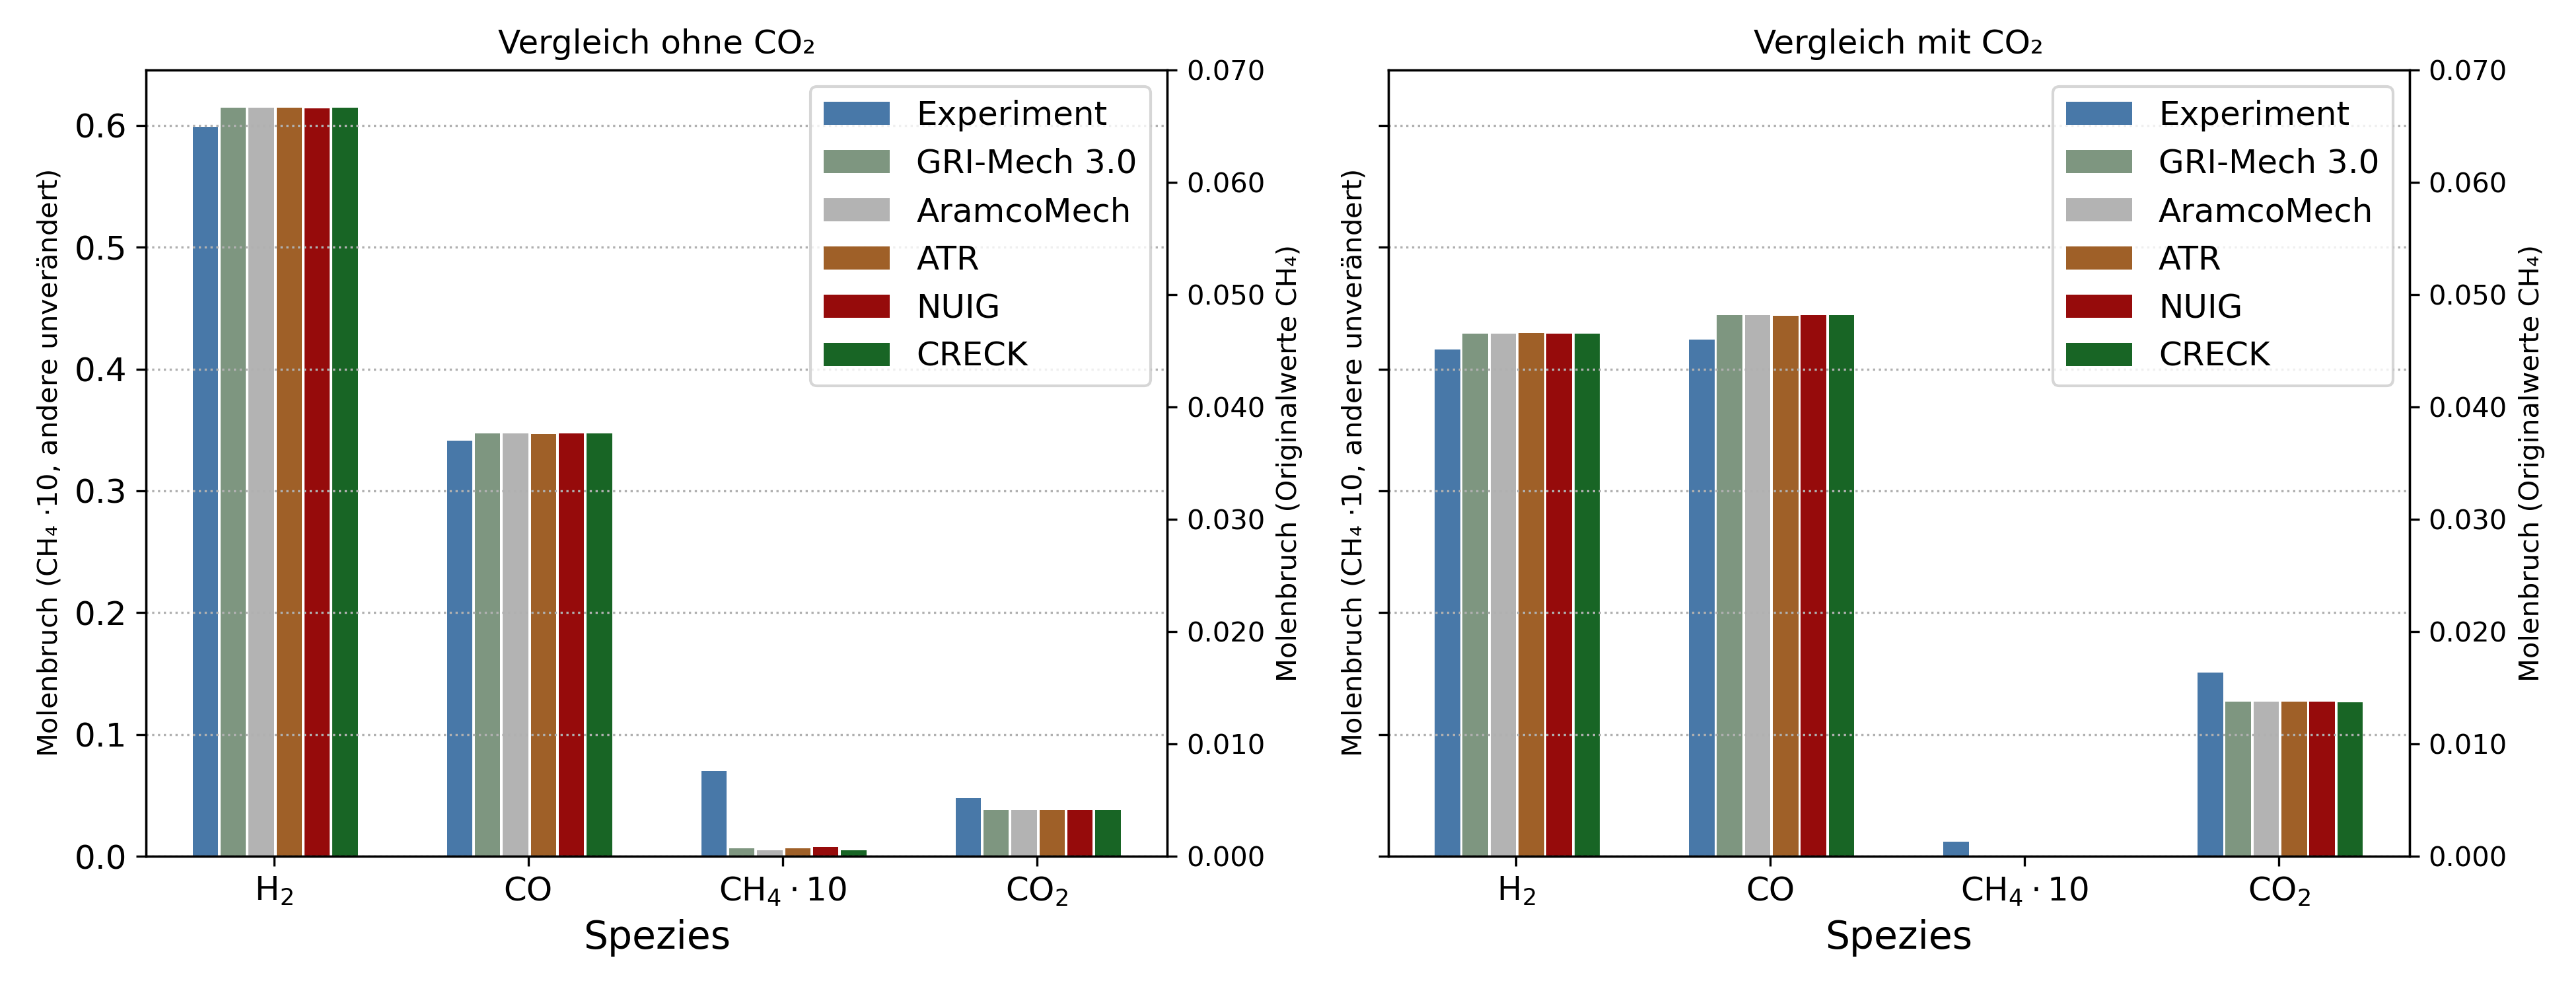
\includegraphics[width=1\linewidth]{img/Vergleich_mech/vergleich_Experimentaldaten_scaled_CH4_gap.png}
            \caption{Vergleich der Massenanteile der Spezies CO, CO$_2$, H$_2$ und CH$_4$ im Produktgas anhand der Berechnungen verschiedener $\mbox{Reaktionsmechanismen}$}
            \label{fig:auswertung_vergleich_exp_stoffe}
        \end{figure}
        Mit der mittleren quadratischen Abweichung (mean squared error, MSE) kann abgeschätzt werden, wie weit ein Wert um einen wahren Wert streut. Dieser ist durch 
        \begin{align}
            MSE = \frac{1}{n}\sum^n_{i=1}\left( Y_i - \hat{Y}_i\right)^2
            \label{eq:mse}
        \end{align}
        definiert, wobei $n$ die Anzahl der Datenpunkte, $Y_i$ die simulierten Werte und $\hat{Y}_i$ die Experimentalwerte sind. 
        In Tabelle \ref{tab:auswertung_mse_mechanismen} sind die mittleren quadratischen Abweichungen beider Simulationen zusammengefasst dargestellt.
        \begin{table}[H]
            \centering
            \caption{Gesamtfehler (mittlerer quadratischer Fehler, MSE) der betrachteten Reaktionsmechanismen für beide Betriebsweisen}
            \label{tab:auswertung_mse_mechanismen}
            \begin{tabular}{lcc}
                \toprule
                \textbf{Mechanismus} & \textbf{Gesamt-MSE (kein CO$_2$)} & \textbf{Gesamt-MSE (mit CO$_2$)} \\
                \midrule
                GRI-Mech 3.0   & 0{,}00006 & 0{,}00023 \\
                AramcoMech         & 0{,}00004 & 0{,}00026 \\
                ATR-Mechanismus & 0{,}00006 & 0{,}00023 \\
                NUIG           & 0{,}00004 & 0{,}00022 \\
                CRECK          & 0{,}00003 & 0{,}00029 \\
                \bottomrule
            \end{tabular}
        \end{table}
        Es ist erkennbar, dass es nur sehr geringe Abweichungen zwischen den Ergebnissen der Mechanismen gibt. In der Literatur sind oftmals Unterschiede zwischen verschiedenen Reaktionsmechanismen beschrieben, allerdings beziehen sich diese Unterschiede oftmals auf direkte Flammeigenschaften wie die Zündverzögerung. Durch die Nachbrennzone gibt es allerdings eine Annäherung der Stoffe an ein chemisches Gleichgewicht. Da diese Gleichgewichtsreaktionen langsamer ablaufen, unterliegt die Parametrisierung dieser Gleichgewichte weniger Ungenauigkeiten, weshalb sich sehr ähnliche Ergebnisse ergeben. 

        Um die Abweichungen der Mechanismen festzustellen, ist eine gesonderte Betrachtung erforderlich. In Abbildung \ref{fig:temp_ch4} sind die Temperatur sowie der Methangehalt am Anfang des PFRs dargestellt. 
        \begin{figure}[H]
            \centering
            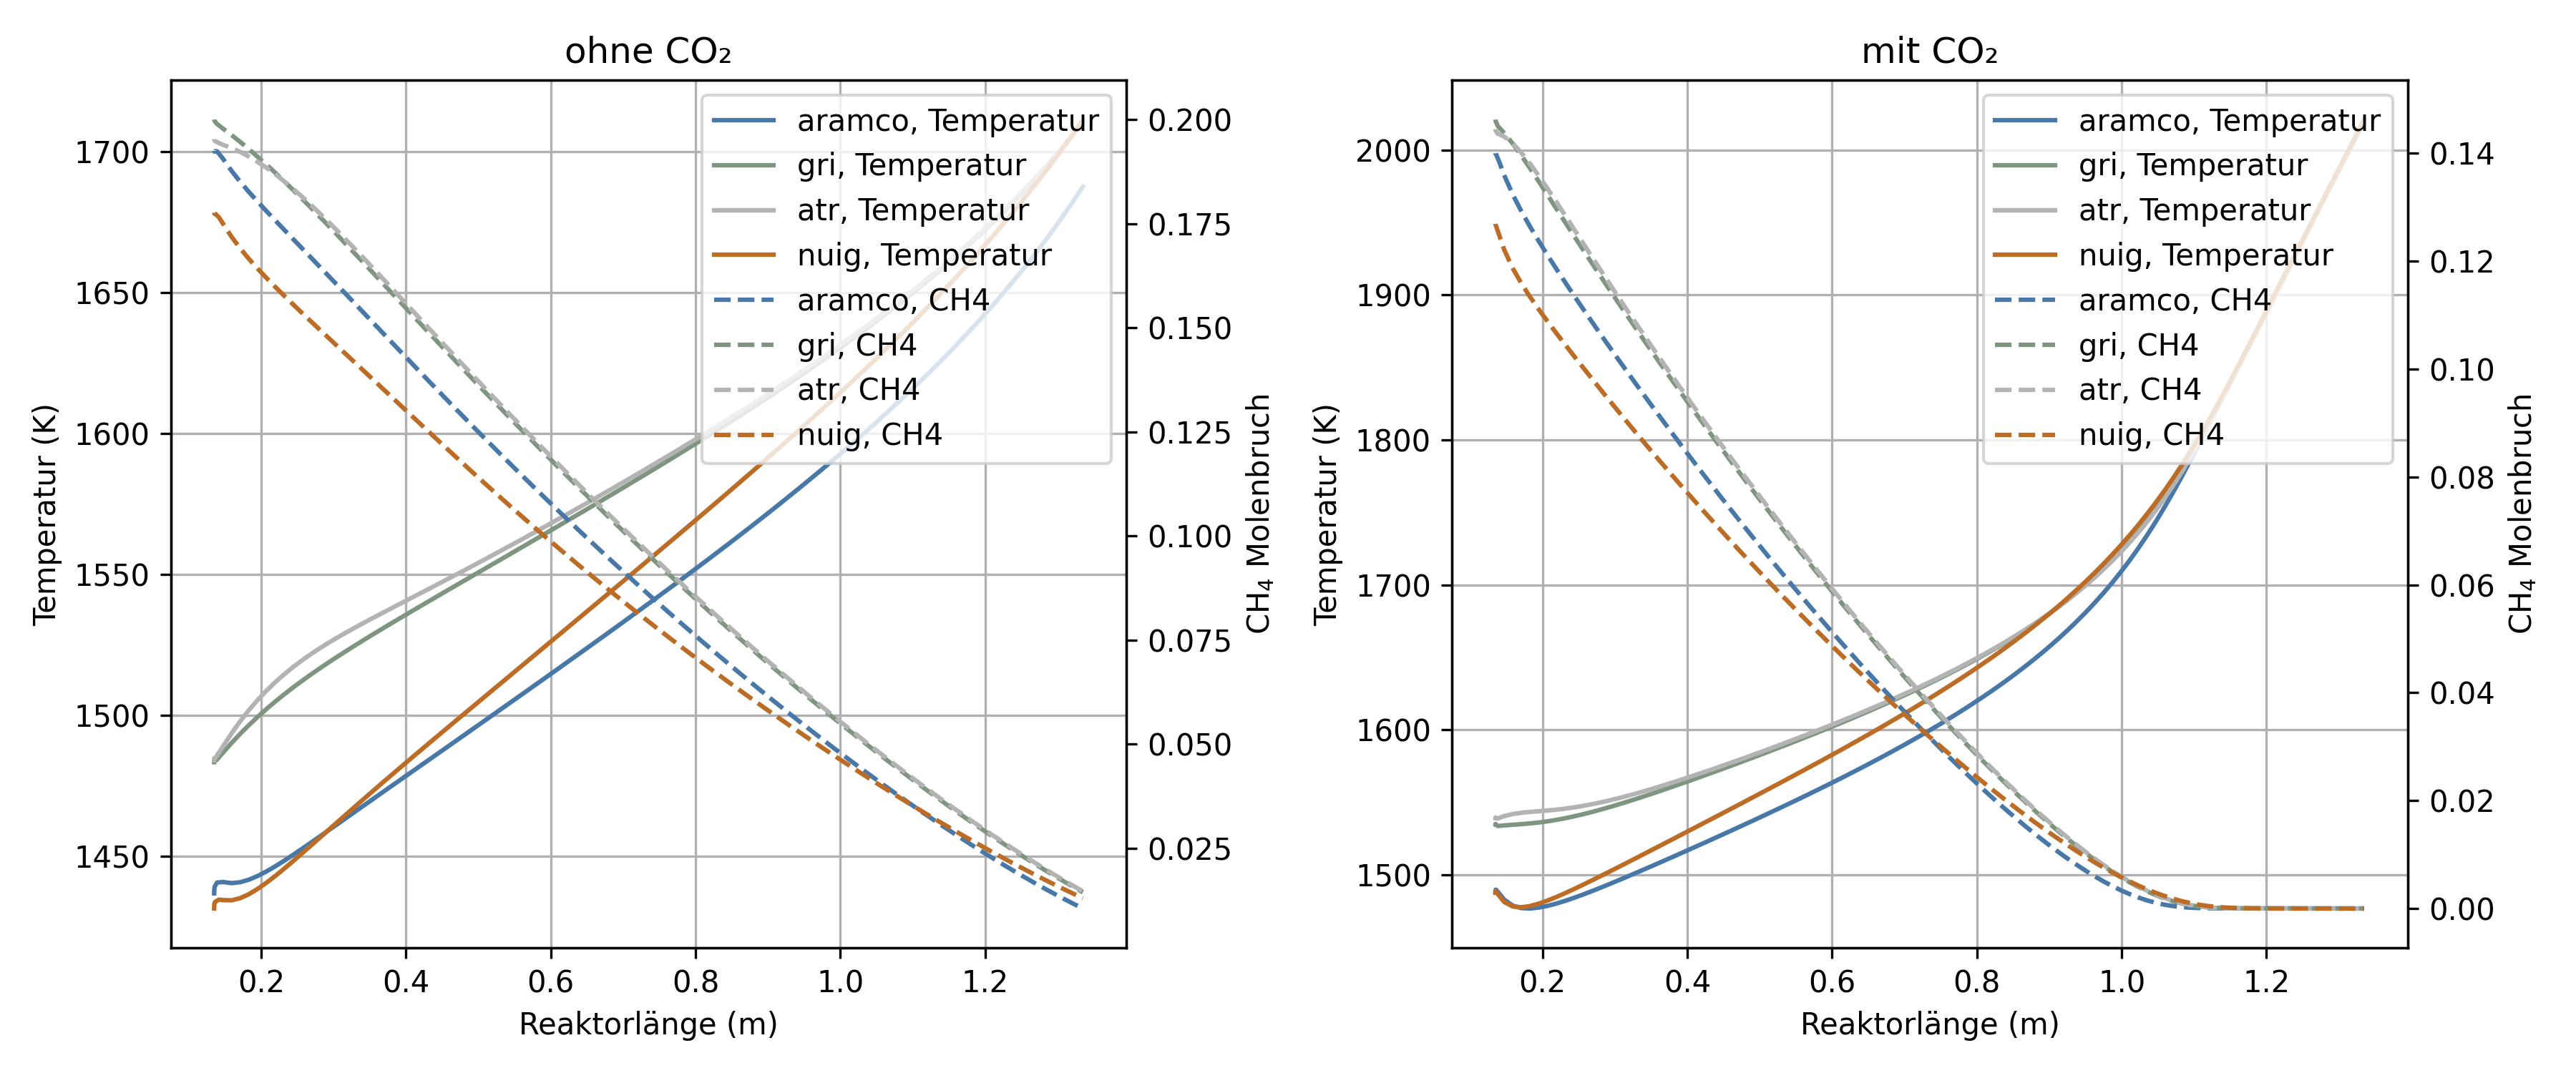
\includegraphics[width=1\linewidth]{img/Vergleich_mech/Temp_CH4.png}
            \caption{Temperatur und Methangehalt im Reaktor zur Unterscheidung der Flammeigenschaften verschiedener Mechanismen}
            \label{fig:temp_ch4}
        \end{figure}
        Dabei ist eine klare Abweichung der Mechanismen untereinander zu erkennen. Da jedoch keine Daten aus Versuchen vorliegen, ist eine Einschätzung der Güte nicht möglich. Dabei ist auch erkennbar, dass durch den höheren Volumenstrom im Fall der CO$_2$-Zugabe eine deutlich kürzere Flammzone vorliegt. Somit stellen sich die Gleichgewichte im zweiten Fall deutlich schneller ein. 

        Auffällig in Tabelle \ref{tab:auswertung_mse_mechanismen} ist, dass die Ergebnisse der Simulationen mit CO$_2$-Zugabe einer höheren Ungenauigkeit unterliegen als die Ergebnisse der Referenzvariante. Zum einen ist dies dadurch erklärbar, dass die verwendeten Reaktionsmechanismen ursprünglich für Anwendungen in der Verbrennung entwickelt wurden. Die CO$_2$-haltigen Gleichgewichte (u. a. die Wassergas-Shift-Reaktion) sind daher nicht optimal parametrisiert, da sie bei der Validierung unter stöchiometrischen Flammenbedingungen nur eine geringe Rolle spielen. Zum anderen führt die Zugabe von CO$_2$ zu einem höheren Massen- und Volumenstrom, wodurch sich die Verweilzeit im Reaktor verkürzt. Dadurch können sich Gleichgewichtsreaktionen nicht vollständig einstellen, was eine größere Abweichung verursacht.
        
        Um einen erheblichen Unterschied der Reaktionsmechanismen festzustellen, wäre ein direkter Vergleich der Flammzone notwendig. Hinsichtlich der großen Ähnlichkeit der Ergebnisse ist eine Erklärung der Abweichung zu den praktisch ermittelten Werten kaum möglich. Dadurch ergibt sich die These, dass dieses lineare Reaktornetzwerk nicht die realen Reaktorbedingungen abbilden kann. Dennoch ist eine sehr hohe Übereinstimmung mit den simulierten Werten erkennbar.

        Neben den Produktgaszusammensetzungen können die simulierten Temperaturdaten mit den gemessenen Temperaturdaten verglichen werden. Die Position der genutzten Thermoelemente ist in Abbildung \ref{fig:erweiterungen_messpunkte} dargestellt. Analog zu Abbildung \ref{fig:auswertung_vergleich_exp_stoffe} sind die Temperaturen in Abbildung \ref{fig:auswertung_vergleich_exp_temp} dargestellt. 
        \begin{figure}[H]
            \centering
            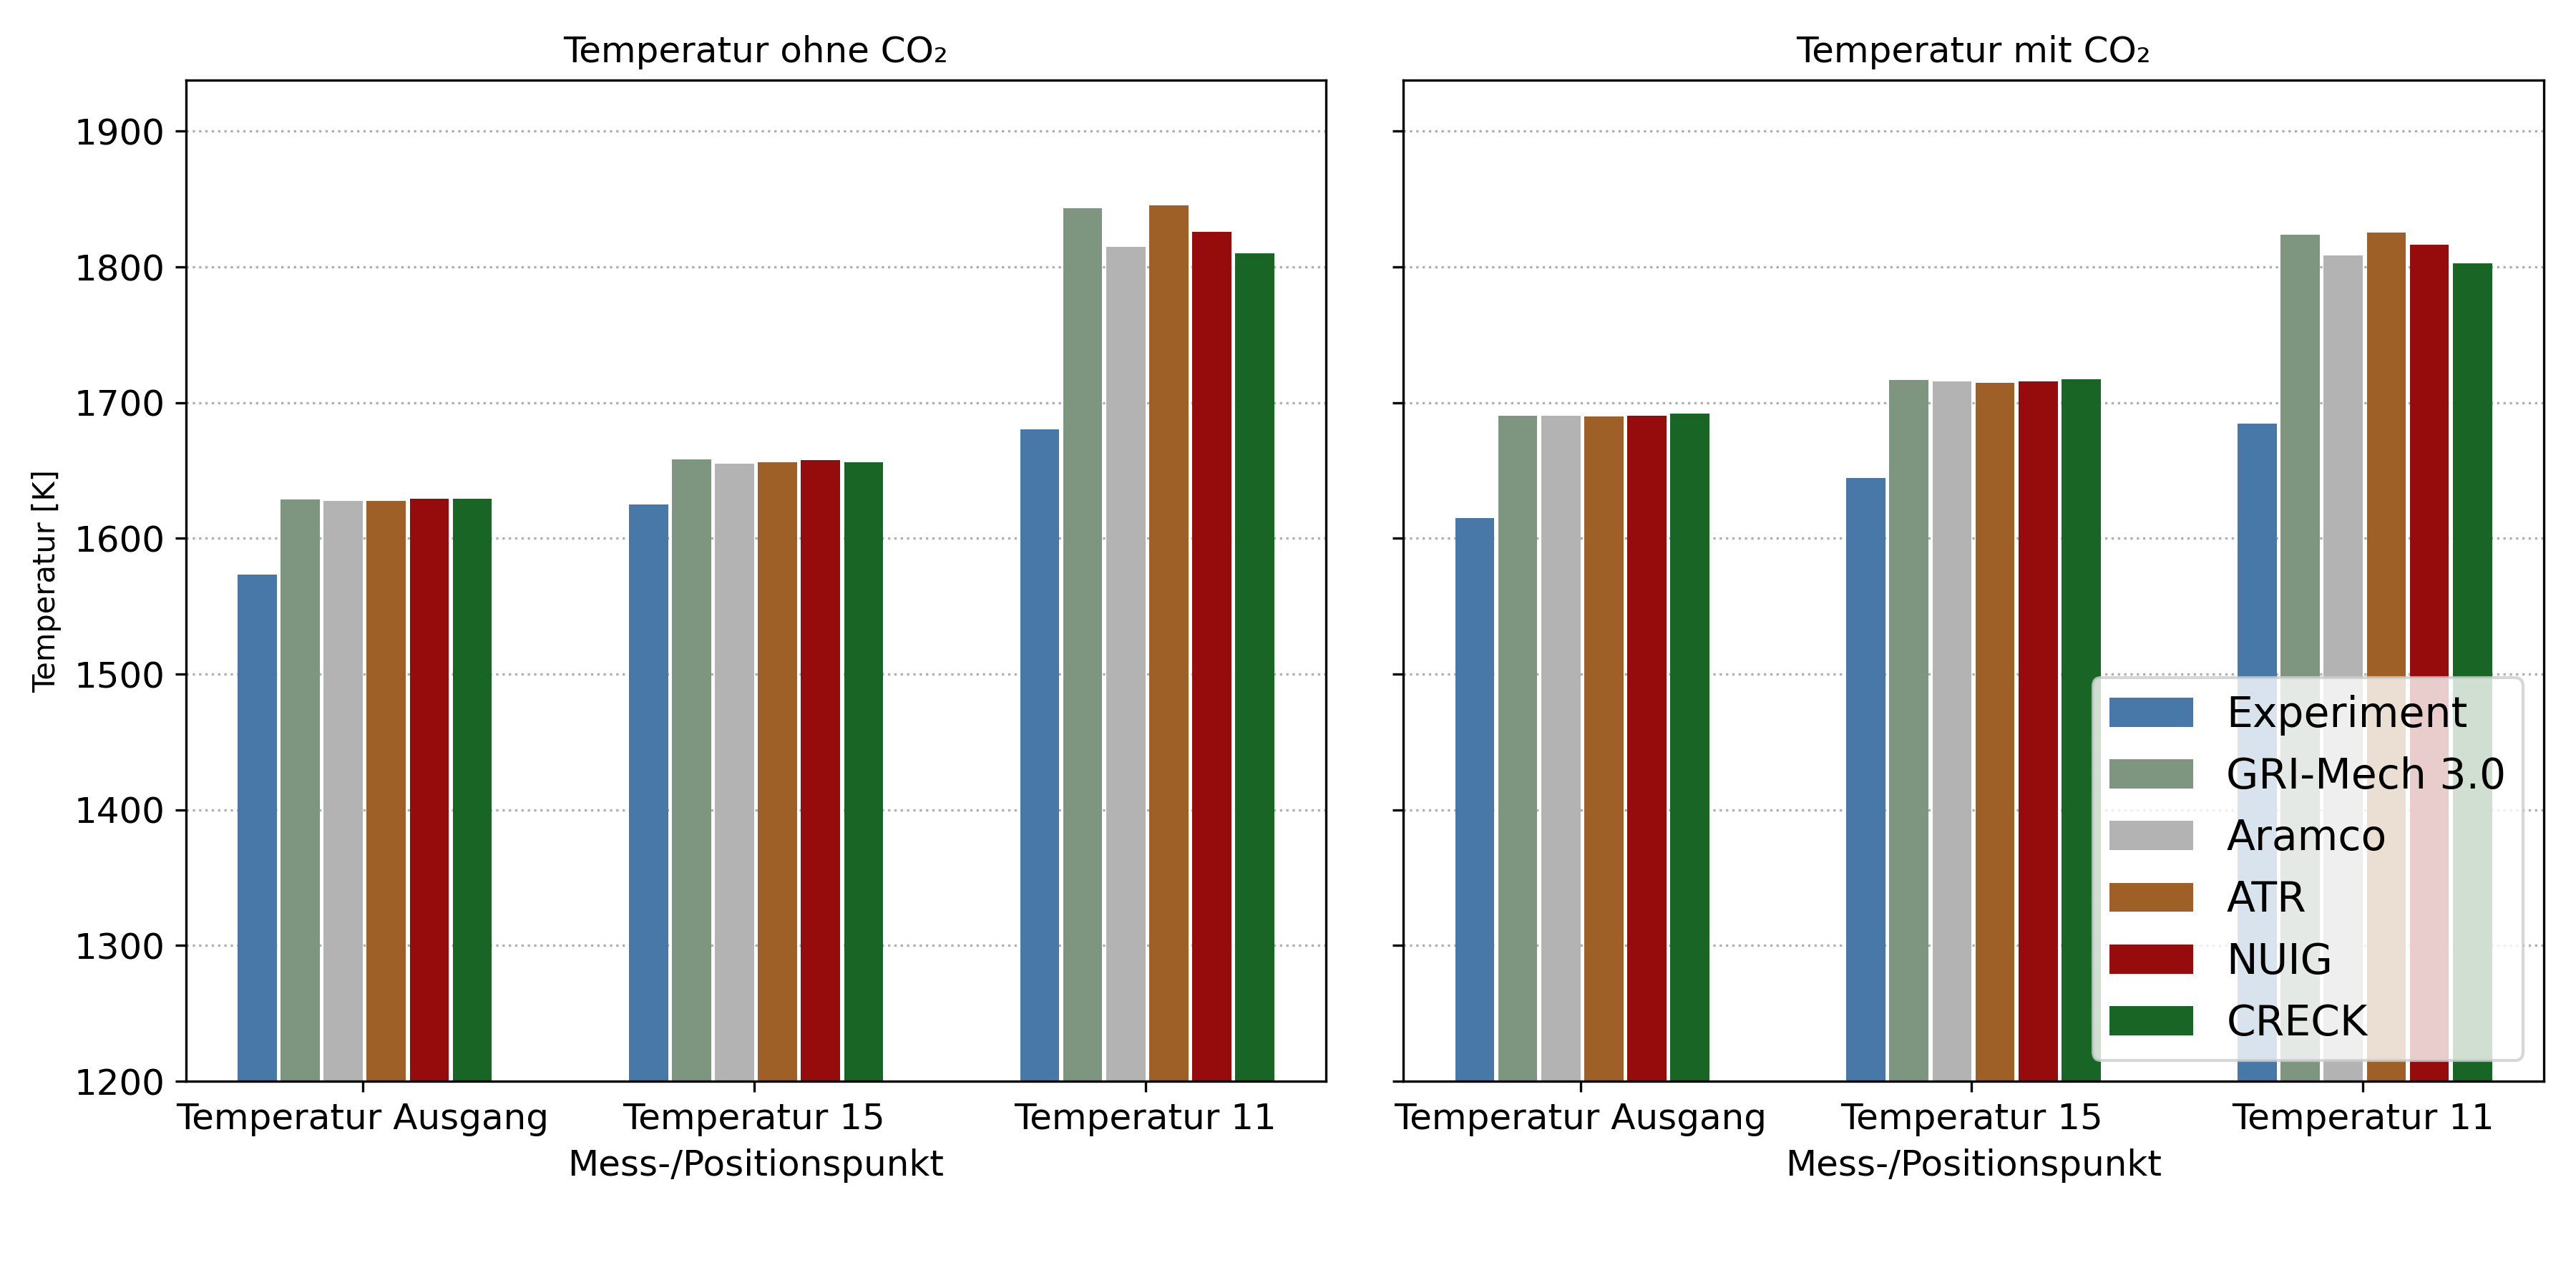
\includegraphics[width=1\linewidth]{img/Vergleich_mech/Vergleich_Temperaturen_gap_manual.png}
            \caption{Vergleich der Temperaturen anhand der Berechnungen verschiedener $\mbox{Reaktionsmechanismen}$ mit experimentellen Daten}
            \label{fig:auswertung_vergleich_exp_temp}
        \end{figure}
        %Auch hier zeigt sich ein ähnliches Verhalten. Fast alle Mechanismen liegen nah beieinander. Ausschließlich der CRECK-Mechanismus weist eine deutliche Abweichung im Fall von zusätzlichem CO$_2$ im Feed auf. Dabei entsprechen die Ergebnisse des CRECK-Mechanismus im Fall 2 am ehesten den gemessenen Temperaturwerten. 

        In beiden Fällen zeigen die Simulationen ein ähnliches Temperaturverhalten mit nur geringen Abweichungen zwischen den Mechanismen. Die größten Differenzen treten am Messpunkt Temperatur 11 auf, wo alle Mechanismen die experimentellen Werte deutlich überschätzen. Während die Ausgangstemperaturen und die Werte am Messpunkt 15 nahezu übereinstimmen, liefern die Mechanismen Aramco und CRECK am Messpunkt 11 die niedrigsten und damit realistischsten Temperaturen.
        %Ohne CO$_2$ (linke Abbildung) liefern GRI-Mech~3.0 und Aramco die besten Übereinstimmungen mit dem Experiment, während CRECK leicht niedrigere Temperaturen berechnet. Mit CO$_2$-Zugabe (rechte Abbildung) verhalten sich die Mechanismen ähnlich, doch der CRECK-Mechanismus liegt hier am nächsten an den gemessenen Temperaturen und bildet den Verlauf insgesamt am realistischsten ab.


        Eine Betrachtung des MSE analog \ref{tab:auswertung_mse_mechanismen} ist hierbei nicht zielführend. Da Temperatur und Stoffmengenanteile verschiedene Größenordnungen besitzen, führt ein einfacher MSE zu einer überproportionalen Betrachtung der Temperaturunterschiede. Ein gewichteter MSE könnte hierbei sinnvolle Vergleichsergebnisse schaffen, die empirische Wichtung muss allerdings validiert werden.

        Da sich alle Temperaturen in einer vergleichbaren Größenordnung bewegen, ist die Betrachtung der Abweichungen in dem Produktgas entscheidender als die Abweichungen der Temperaturen. 

        Aufgrund der Literaturrecherche (vgl. Abschnitt \ref{sec:reaktionsmechanismen_literatur}), der Modellkomplexität und der Ergebnisse in Tabelle \ref{tab:auswertung_mse_mechanismen} wurde Aramco als Mechanismus für die weitere Verwendung ausgewählt. Dieser stellt dabei einen guten Kompromiss aus Rechenzeit, Genauigkeit und Stabilität dar. 
        Für eine ausschließliche Betrachtung des Referenzfalls wäre auch der Einsatz des CRECK-Mechanismus denkbar. Aufgrund seiner höheren Abweichungen im Fall mit CO$_2$-Zugabe wird seine Verwendung jedoch nicht bevorzugt, er kann jedoch als möglicher Alternativmechanismus herangezogen werden.
\iffalse
        Da alle Simulationen mit den verschiedenen Reaktionsmechanismen in einem Identischen Reaktornetzwerk unter konstanten Bedingungen durchgeführt wurden, ist ein Vergleich der Gaszusammensetzungen in der Reforming Zone möglich. In Abbildung \ref{fig:auswertung_verläufe_mechanismen_keinco2} sind diese Zusammensetzungen für den Fall, dass kein zusätzliches CO$_2$ dem Feed zugegeben wird, dargestellt. 
        \begin{figure}[H]
            \centering
            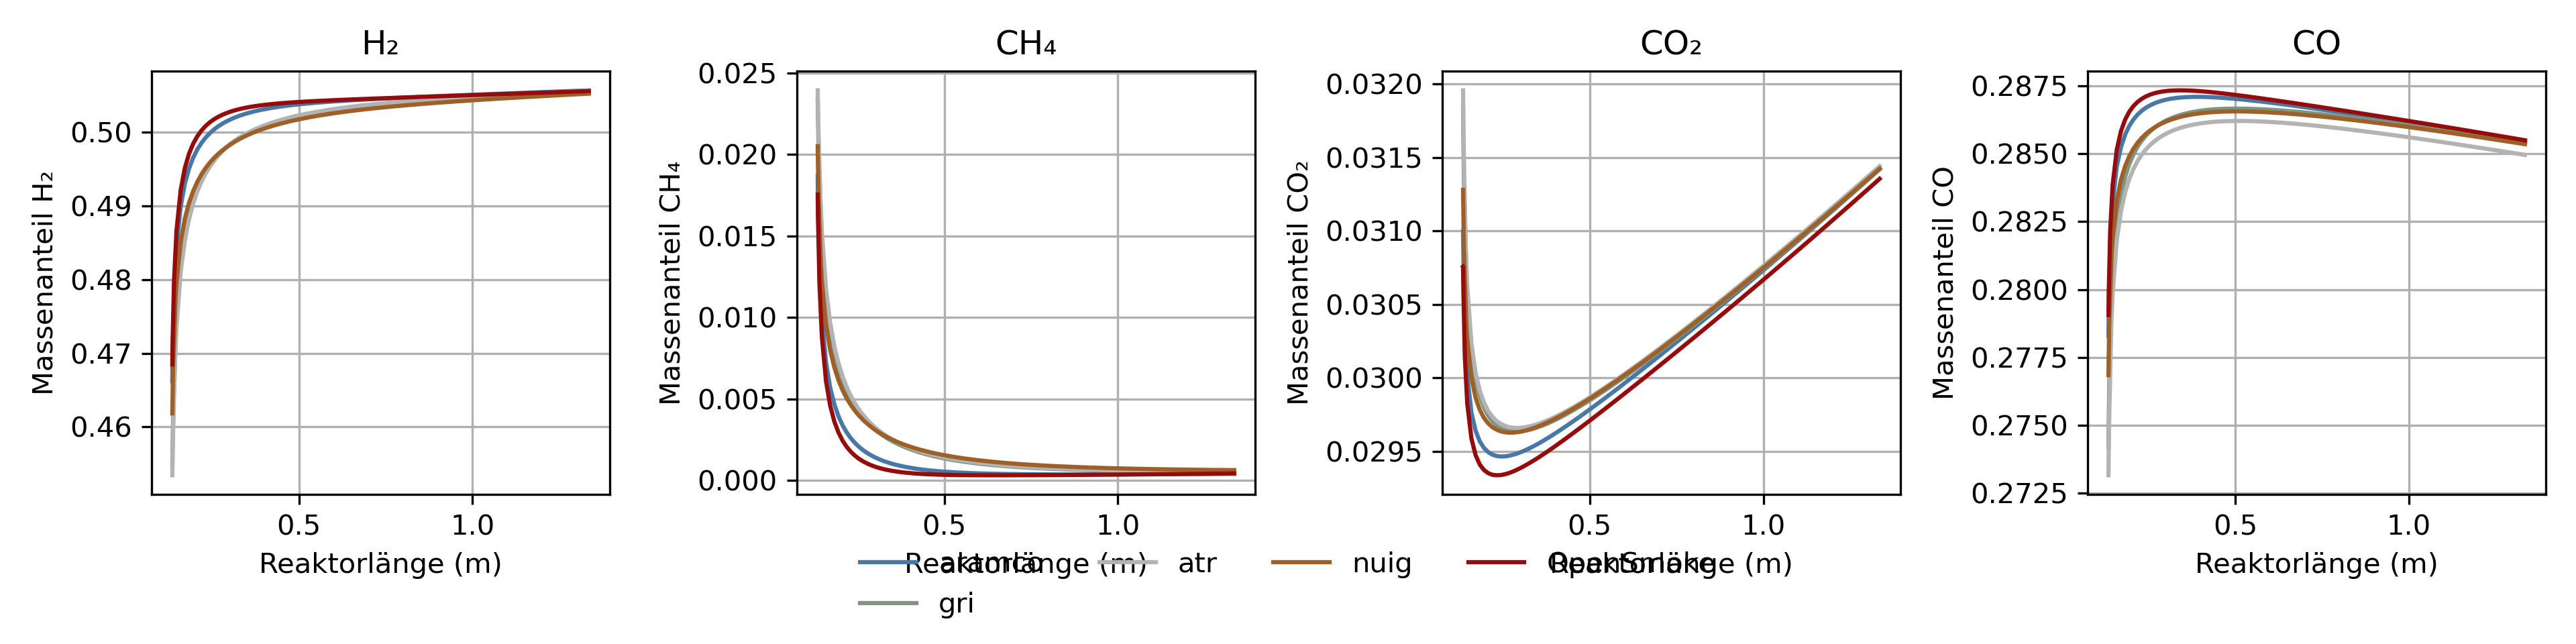
\includegraphics[width=1\linewidth]{img/Vergleich_mech/H2_CH4_CO_CO2_keinCO2.png}
            \caption{Vergleich der Massenprofile der Spezies CO, CO$_2$, H$_2$ und CH$_4$ entlang der Strömungszone anhand der Berechnungen verschiedener $\mbox{Reaktionsmechanismen}$}
            \label{fig:auswertung_verläufe_mechanismen_keinco2}
        \end{figure}
        In Abbildung \ref{fig:auswertung_verläufe_mechanismen_keinco2} kann man gut erkennen, dass es zwar am Anfang des Reaktors signifikante Abweichungen voneinander gibt, während zum Ende des Reaktors kaum Abweichungen vorliegen. Die Abweichung am Anfang des PFRs ist durch die in der Literatur festgestellten Unterschiede im Zündverhalten der Mechanismen begründbar. Die Annäherung zu einem ähnlichen Ergebnis aller Mechanismen ist dadurch begründbar, da sich die Zusammensetzungen in der Nachbrennzone zunehmend dem thermodynamischen Gleichgewicht annähern, wodurch die Unterschiede zwischen den Mechanismen geringer werden.

        \alert{Ein vergleichbares Verhalten der Mechanismen kann auch für den zweiten Fall festgestellt werden}
        \begin{figure}[H]
            \centering
            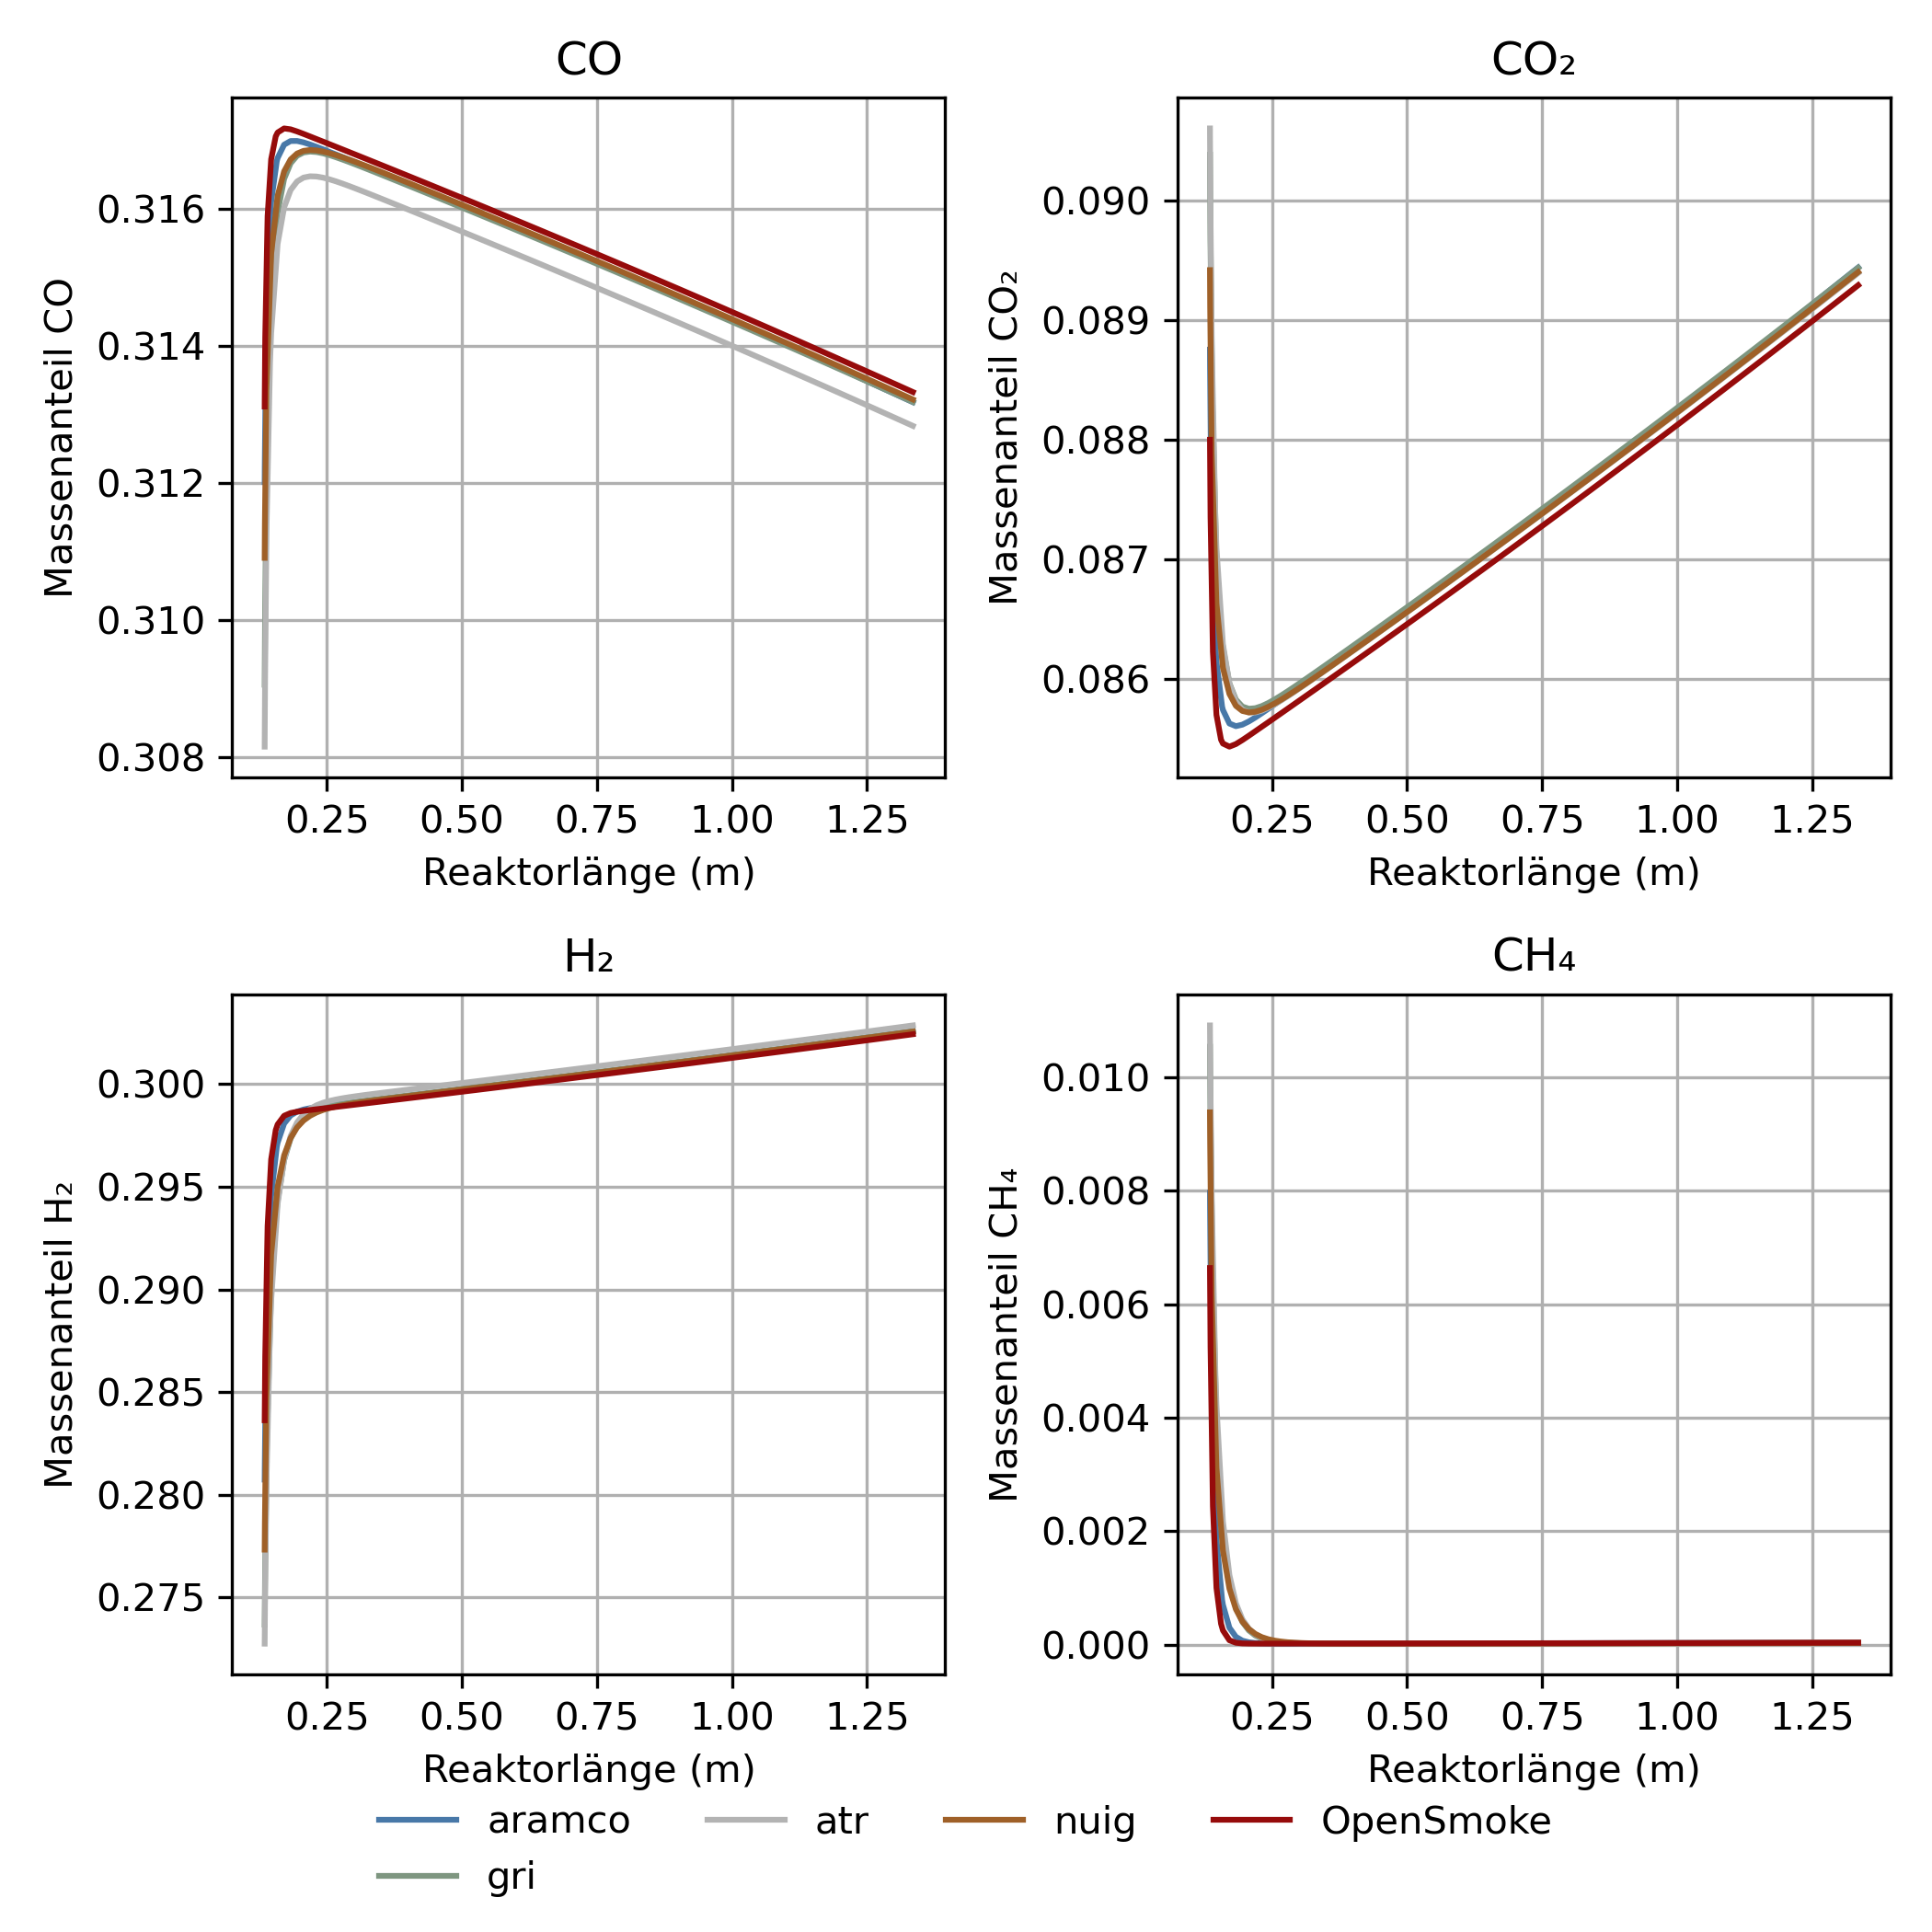
\includegraphics[width=0.6\linewidth]{img/Vergleich_mech/H2_CH4_CO_CO2.png}
            \caption{Vergleich der Massenprofile der Spezies CO, CO$_2$, H$_2$ und CH$_4$ entlang der Strömungszone anhand der Berechnungen verschiedener $\mbox{Reaktionsmechanismen}$}
            \label{fig:auswertung_verläufe_mechanismen_keinco2}
        \end{figure}

        Insgesamt ist die Abweichung der simulierten Ergebnisse im Vergleich zu den gemessenen Werten extrem klein. In Tabelle \ref{tab:auswertung_mse_mechanismen} ist der mittlere quadratische Fehler aller Reaktionsmechanismen für beide Simulationsfälle dargestellt. Die Vollständigen Tabellen aller Fehler für jede Spezies befinden sich im Anhang.
        \begin{table}[H]
            \centering
            \caption{Gesamtfehler (mittlerer quadratischer Fehler, MSE) der betrachteten Reaktionsmechanismen für beide Betriebsweisen}
            \label{tab:auswertung_mse_mechanismene}
            \begin{tabular}{lcc}
                \toprule
                \textbf{Mechanismus} & \textbf{Gesamt-MSE (kein CO$_2$)} & \textbf{Gesamt-MSE (mit CO$_2$)} \\
                \midrule
                GRI-Mech 3.0   & 0{,}00006 & 0{,}00023 \\
                Aramco         & 0{,}00004 & 0{,}00026 \\
                ATR-Mechanismus & 0{,}00006 & 0{,}00023 \\
                NUIG           & 0{,}00004 & 0{,}00022 \\
                Smoke          & 0{,}00003 & 0{,}00029 \\
                \bottomrule
            \end{tabular}
        \end{table}
        Bemerkenswert ist jedoch, dass die Ergebnisse bei der Simulation mit CO$_2$-Zugabe um ein vielfaches höher sind als bei der Referenzvariante. Dadurch, dass diese Reaktionsmechanismen ursprünglichen für die Anwendung der Verbrennung entwickelt wurden, sind die CO$_2$-haltigen Gleichgewichte (u.a. Wassergas-Shift-Reaktion) nicht optimal parametrisiert, da diese bei stöchiometrischer Flammenvalidierung kaum Gewicht haben.
        %Eine Mögliche Erklärung für diese Beobachtung ist, dass die Gleichgewichtsreaktionen, die CO$_2$ beinhalten, in der ursprünglichen Anwendung weniger Relevanz hatten, und diese dadurch weniger exakte Reaktionsparameter vorweisen. 

        Insgesamt stützt diese Auswertung dabei die These, dass alle Reaktionsmechanismen eine gute Genauigkeit aufweisen und erklärt ebenfalls die verschiedenen Ergebnisse verschiedener Studien. Demnach ist die Auswahl des passendsten Mechanismus immer eine Frage der Prozessbedingungen und der beste Mechanismus kann ohne Vorbetrachtungen nicht explizit erkannt werden. Beispielsweise ist in den Ergebnissen dieses Vergleiches der Fehler des CRECK-Mechanismus in einem Fall klein, in dem anderen Fall verhältnismäßig groß.

        Darüber hinaus zeigen die sehr kleinen Fehler zudem, dass es bei der Wahl des geeigneten Mechanismus vielmehr auf die Art der geforderten Reaktionen und die Effizienz der Berechnungen ankommt als auf die eigentlichen kinetischen Parameter der Studien, da diese in vielen Fällen ähnliche Ergebnisse liefern. 

        Obwohl der Aramco-Mechanismus im Fall der CO$_2$-unterstützten POx etwas größere Abweichungen aufweist als andere Mechanismen, wird er für die folgenden Simulationen dieser Arbeit verwendet. Ausschlaggebend hierfür ist der, wie zuvor beschrieben, gute Kompromiss aus Genauigkeit, Detaillierungsgrad, numerischer Stabilität und Recheneffizienz. Darüber hinaus wird der Aramco-Mechanismus in der Literatur häufig als Referenzmechanismus herangezogen, wodurch er sich besonders für vergleichende Studien und die Untersuchung unterschiedlicher Prozessbedingungen eignet.
\fi 
    \section{Erweiterungen des Reaktornetzwerkmodells}
        Bis zu diesem Zeitpunkt wurde für alle Simulationen ein linear aufgebautes Reaktornetzwerk, bestehend aus einem PSR und einem PFR, genutzt. Da jedoch aufgrund einer CFD-Analyse (siehe Kapitel \ref{sec:vorbetrachtungen}) bekannt ist, dass der Reaktor ein anderes Strömungsverhalten aufweist, wurde mithilfe weiterer Reaktoren das Reaktornetzwerk erweitert, um die Bedingungen im Reaktor besser abbilden zu können.

        Da in den Reaktornetzwerken keine vergleichbaren PFRs mehr enthalten sind, ist eine Auswertung der Profile dieser Reaktoren kaum noch möglich und der Vergleich dieser Netzwerke bezieht sich allein auf die Produktgaszusammensetzung. In Abbildung \ref{fig:auswertung_erweiterungen_spezies} sind diese Produktgaszusammensetzungen dargestellt. 
        \begin{figure}[H]
            \centering
            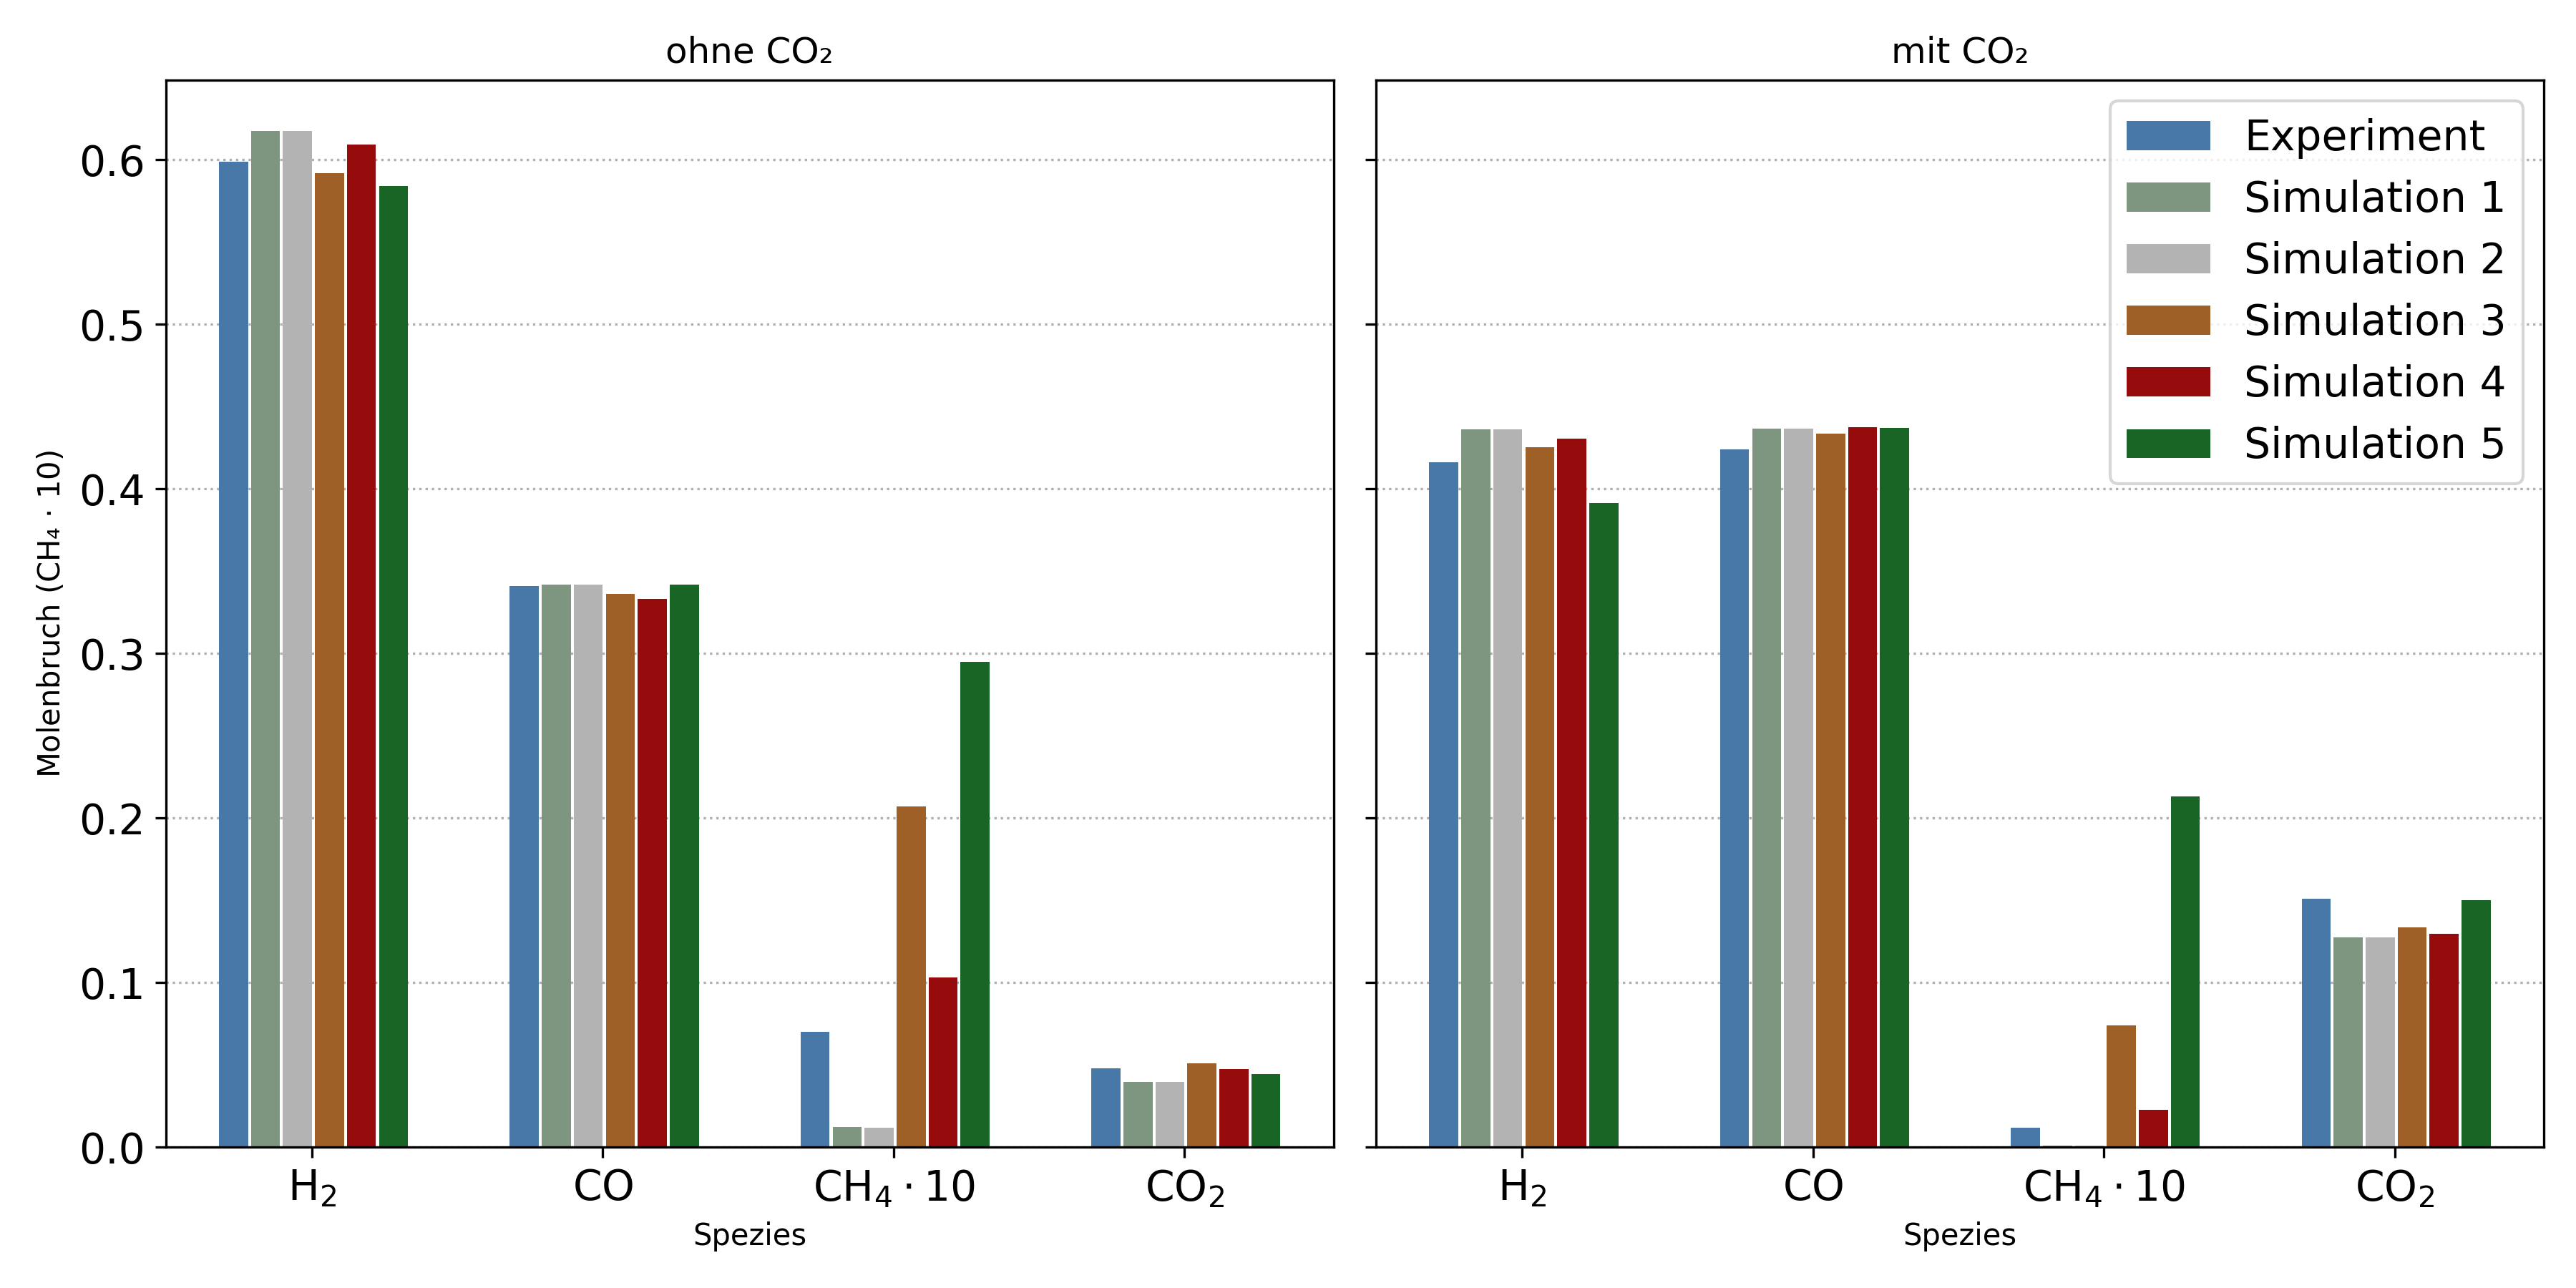
\includegraphics[width=1\linewidth]{img/Erweiterungen/Vergleich_Erweiterungen.png}
            \caption{Gemessene und simulierte Produktgaszusammensetzung verschiede\-ner Reaktornetzwerke}
            \label{fig:auswertung_erweiterungen_spezies}
        \end{figure}
        Um die verschiedenen Netzwerke untereinander zu vergleichen wird wieder der mit\-tlere quadratische Fehler zwischen den Simulationen ermittelt. Dieser ist in Tabelle \ref{tab:tvd_modelle} dargestellt.
        \begin{table}[H]
            \centering
            \caption{Berechneter mittlerer quadratische Fehler (MSE) der Modelle mit und ohne CO$_2$}
            \label{tab:tvd_modelle}
            \begin{tabular}{lcc}
                \toprule
                \textbf{Modell} & \textbf{MSE (ohne CO$_2$)} & \textbf{MSE (mit CO$_2$)} \\
                \midrule
                1 & 0,00011 & 0,00028 \\
                2 & 0,00011 & 0,00028 \\
                3 & 0,00007 & \textbf{0,00013} \\
                4 & \textbf{0,00004} & 0,00021 \\
                5 & 0,00018 & 0,00029 \\
                \bottomrule
            \end{tabular}
        \end{table}
        Man kann erkennen, dass es keine kontinuierliche Verbesserung der Modelle gibt. Das komplexeste Rechenmodell weist dabei sogar den größten Fehler mit einer sehr großen Überschätzung des Methanaustritts auf. Wie in Kapitel \ref{sec:auswertung_mechanismus} bereits erläutert, sind die Abweichungen größer, wenn zusätzlich zum Referenz-POx-Prozess noch Kohlenstoffdioxid hinzugegeben wird. Dies kann in jedem Modell festgestellt werden. Aus Tabelle~\ref{tab:tvd_modelle} geht hervor, dass im zweiten Fall Modell~3 die geringste Gesamtabweichung liefert, obwohl in Abbildung~\ref{fig:auswertung_erweiterungen_spezies} erkennbar ist, dass der Methanschlupf von Modell~4 näher am experimentellen Wert liegt. Da die Methankonzentrationen sehr gering sind, wirkt sich diese Abweichung insgesamt nur geringfügig auf die Gesamtbewertung aus.

        Zwischen Modell 1 und Modell 2 können keine Veränderungen in der Abweichung festgestellt werden. Da sich Modell 2 um einen hinzugefügten Bypass von Modell 1 unterscheidet, ergibt sich die Beobachtung, dass der Stoffstrom im Bypass keine Auswirkungen auf die Reaktionsbedingungen hat. Da im Bypass kein Sauerstoff als Reaktionspartner vorhanden ist, wird das Methan dementsprechend nicht im Bypass, sondern in der Nachbrennzone umgesetzt. Dabei kommen folgende Reaktionen neben Radikalbildungen infrage:
        \begin{align}
            \mathrm{CH_4 + H_2O} & \leftrightharpoons\mathrm{ CO + 3\ H_2} \\ 
            \mathrm{CH_4 + CO_2} & \leftrightharpoons \mathrm{2\ CO +2\ H_2}
        \end{align}
        Diese endothermen Reaktionen laufen in der Nachbrennzone aufgrund der dort vorherrschenden hohen Temperaturen trotz ihrer kinetischen Trägheit mit hinreichender Geschwindigkeit ab und tragen somit zusätzlich zum Abbau des Methans bei.

        Eine Erweiterung dieses Modells mit einem PSR als Rezirkulationszone sorgt für eine höhere Genauigkeit beider Simulationsfälle. So ergibt sich bei dem Fall mit CO$_2$ das genaueste Modell, während es im Referenzfall das zweitbeste Modell darstellt. Insgesamt überschätzt dieses Modell den Schlupf von Methan deutlich, stellt dafür die Komponenten Wasserstoff, Kohlenstoffmonoxid und Kohlenstoffdioxid gut dar. Die Rückführung des bereits entstandenen Produktgases durch die Rezirkulationszone sorgt zwar für eine höhere Temperatur in dem Bypass, verdünnt aber gleichzeitig noch nicht umgesetztes Methan, weshalb sich der zu hohe Schlupf von Methan ergibt. 

        Wenn die Rezirkulationszone stärker im Austausch mit der Nachbrennzone steht, was durch Reaktornetzwerk 4 umgesetzt wurde, indem ein zusätzlicher Strom durch die Teilung des PFRs hinzugefügt wurde, wird die Umsetzung des Methans durch beide Simulationen am genauesten berechnet. Insgesamt ist dieses reduzierte Modell am besten geeignet, um die herkömmliche POx ohne Zugabe von CO$_2$ im Feed zu modellieren. Auch im zweiten Fall wird eine hohe Genauigkeit erreicht, allerdings mit weniger Übereinstimmung als mit dem vorherigen Modell. 

        Durch die Auftrennung des PFRs wird ein Teil des entstandenen Produktgases zurück in die Bypasszone geführt. Dadurch wird noch nicht umgesetztes Methan mit Restbeständen Sauerstoff aus dem Produktgas in Verbindung gebracht, und noch nicht umgesetztes Methan im PFR wird erneut durch den Reaktor geleitet. Insgesamt ist somit eine Abschätzung der Produktgaszusammensetzung möglich. Da in diesem Modell die Interaktion mit der Rezirkulationszone erweitert wurde, spielen chemische Gleichgewichte eine größere Rolle. Da diese im Fall der trockenen Reformierung größere Fehler aufweisen, kann die geringere Genauigkeit des CO$_2$-Falls erklärt werden. 

        Durch die Auftrennung der Rezirkulationszone in zwei Teile, sowie die umfangreiche Interaktion beider Zonen mit der Strömungszone, entsteht das in dieser Arbeit komplexeste Modell. Die Modellierung mit diesem Modell führt zu den größten Abweichungen aller Modelle. Insbesondere der Schlupf von Methan wird deutlich überschätzt.

        Aufgrund der hohen Komplexität des Modells durch zwei getrennte Rezirkulationszonen und viele Interaktionen der Reaktoren untereinander, sind im Vergleich zu den einfacheren Modellen deutlich mehr Annahmen zu treffen. Dadurch, dass die einfacheren Modelle sehr genaue Ergebnisse liefern, hat die große Anzahl an getroffenen Annahmen einen insgesamt negativen Effekt auf die Modellgüte. Darunter befindet sich die Aufteilung der Ströme und die Größen der Reaktoren. Eine Trennung der Rezirkulationszone kann sich zudem negativ auf den Wärmeübergang in dem Reaktor auswirken. Ein sehr komplexes Modell hat zudem starken Einfluss auf die Rechenzeit und numerische Stabilität. 

        In Abbildung \ref{fig:auswertung_erweiterungen_temperaturen} sind die simulierten Temperaturen dargestellt. 
        \begin{figure}[H]
            \centering
            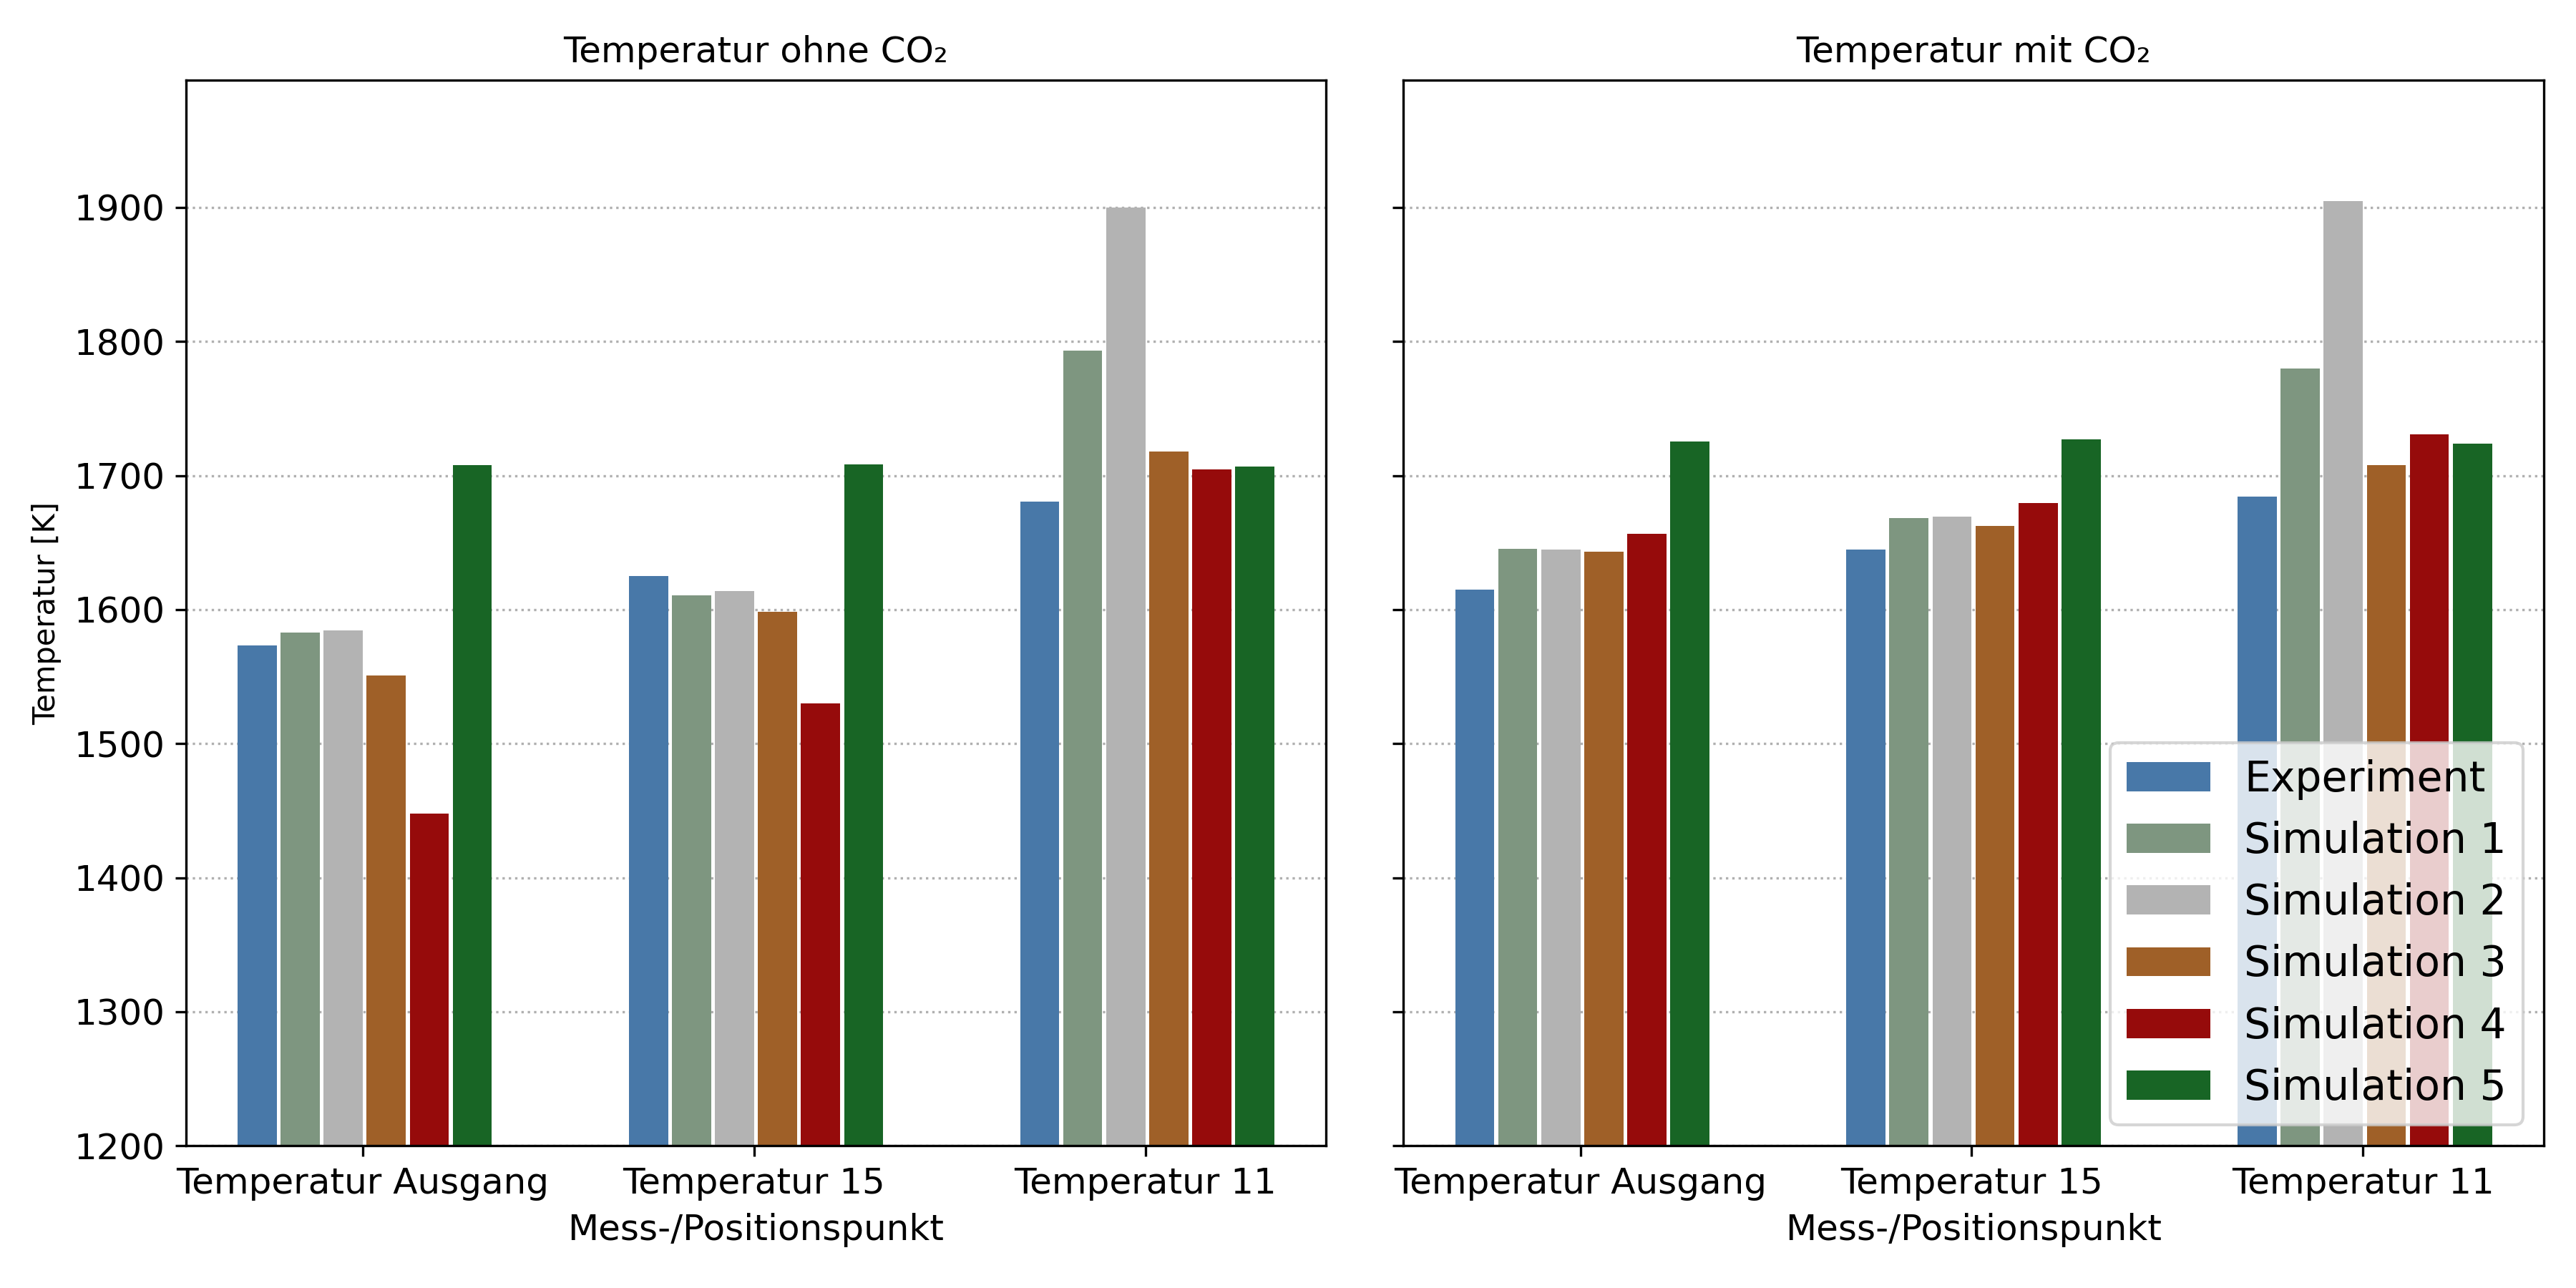
\includegraphics[width=1\linewidth]{img/Erweiterungen/Vergleich_Temperaturen.png}
            \caption{Gemessene und simulierte Temperaturen verschiede\-ner Reaktornetzwerke}
            \label{fig:auswertung_erweiterungen_temperaturen}
        \end{figure}
        Hierbei befinden sich alle Temperaturen in einer ähnlichen Größenordnung. Dabei weist das komplexeste Modell wieder von den Experimentaldaten aufgrund nicht optimalen Modellannahmen ab.
    \section{Rechenzeit}
        Damit umfangreiche Parameterstudien durchgeführt werden können, ist eine kurze Rechenzeit von hoher Bedeutung. Während Reaktornetzwerkmodell~1 eine Rechenzeit von etwa 7~s und Reaktornetzwerkmodell~2 eine Rechenzeit von etwa 14~s aufweist, beträgt die Rechenzeit der Modelle mit Rückkopplung über 10~Minuten. In Tabelle \ref{tab:rechendauer} sind die Rechenzeiten der Modelle aufgelistet. Dabei gab es keine Unterschiede bei der Berechnung beider Fälle.
        \begin{table}[H]
            \centering
            \caption{Übersicht über die gemessene Rechendauer der verschiedenen Reaktormodelle}
            \begin{tabular}{c c}
                 \toprule
                 Modell & Rechenzeit in Sekunden \\
                 \midrule
                 1 & 7 \\
                 2 & 14 \\ 
                 3 & 630 \\ 
                 4 & 720 \\ 
                 5 & 750 \\
                 \bottomrule
            \end{tabular}
            \label{tab:rechendauer}
        \end{table}
        Da die Rechenzeit nicht nur von der Modellkomplexität, sondern auch von der genutzten Hardware, getroffenen Abschätzungen, numerischen Einstellungen und vielen anderen Faktoren abhängig ist, dient diese Übersicht nicht als klare Angabe der Rechenzeit, sondern vielmehr zur Darstellung eines Trends. 

        Es ist erkennbar, dass die linearen Modelle sehr schnelle Lösungen ergeben, da diese keine iterative Lösung aufweisen. Durch die Iteration ab Modell 3 ergeben sich deutlich höhere Rechenzeiten. Eine Abweichung zwischen Modell~4 und 5 ist kaum zu erkennen, da die Berechnung eines einzelnen PSRs kaum Rechenzeit in Anspruch nimmt. 
        
        Durch den damit verbundenen deutlich höheren Rechenaufwand sind diese kom\-plexeren Modelle nur eingeschränkt für Parameterstudien geeignet. Aufgrund der hohen Modellgüte der einfachen Netzwerke ist es daher sinnvoller, die Parameterstudien mit einem dieser Modelle durchzuführen. Soll ein höherer Detailgrad der Ergebnisse erzielt werden, können im Anschluss auf Basis der Parameterstudie gezielte Einzelsimulationen mit komplexeren Reaktornetzwerken erfolgen. Zwar kann durch eine Anpassung der Lösungsparameter sowie der numerischen Dämpfung eine Beschleunigung der Berechnung erreicht werden, da die optimalen Parameter jedoch stark von den Prozessbedingungen abhängen, ist dieser Ansatz im Rahmen einer Parameterstudie nicht relevant. Eine signifikante Abweichung der Rechenzeiten der Modelle~3 bis 5 konnte nicht festgestellt werden, da der überwiegende Teil der Rechenzeit durch die iterative Annäherung an den stationären Zustand bestimmt wird, was bei allen Modellen einen vergleichbaren Aufwand verursacht. Zudem ist die Lösung des zusätzlich eingefügten PSRs im Vergleich zu den bereits vorhandenen PFRs deutlich weniger rechenintensiv, wodurch sich der Gesamtaufwand nur geringfügig verändert.
    \section{Parameterstudie CO$_\mathbf 2$}
        Ziel des Projekts \textit{SCOORE} ist die Entwicklung neuer Prozesse zum Recycling bzw. Nutzen von Kohlenstoffdioxid \cite{Scoore_Enargus}. Damit der Prozess sowohl das Recycling von CO$_2$ ermöglichen soll, als auch wirtschaftlich und produktionstechnisch in Produktionsketten integriert werden kann, ist eine Parameterstudie zum Untersuchen des CO$_2$-Feedmassen\-stroms essentiell.

        Da in den vorherigen Kapiteln bereits gezeigt wurde, dass ein lineares Reaktornetzwerk eine ausreichend hohe Genauigkeit bei geringer Rechendauer liefert, wird dieses Modell für die nachfolgende Parameterstudie verwendet. Aufgrund der geringen Rechenzeit eignet es sich besonders für umfangreiche Simulationsreihen und ermöglicht eine effiziente Untersuchung der relevanten Einflussgrößen.
        
        %Da in Kapitel \ref{sec:auswertung_mechanismus} festgestellt wurde, dass ein einfaches lineares Reaktornetzwerk ausreicht, um Prozesse mit ausreichend Genauigkeit zu quantifizieren, kann für diese Parameterstudie auf dieses einfache Reaktornetzwerk zurückgegriffen werden, um effizient eine Parameterstudie durchzuführen. 

        Da der eingesetzte Rohstoff Methan (bzw. Erdgas) sowohl kostenintensiv ist, als auch ein hohes Treibhauspotential besitzt, ist es sowohl aus ökologischen und ökonomischen Gründen essentiell, einen Schlupf von Methan zu minimieren. Darüber hinaus ergibt sich ein Grenzwert von 0,5~Vol.-\% aus den Einschränkungen der nachgeschalteten Prozesse, insbesondere der Gasreinigungseinheiten. In Abbildung \ref{fig:auswertung_co2_methanschupf} ist der Methanschlupf in Abhängigkeit des CO$_2$-Massenstroms dargestellt. 
        \begin{figure}[H]
            \centering
            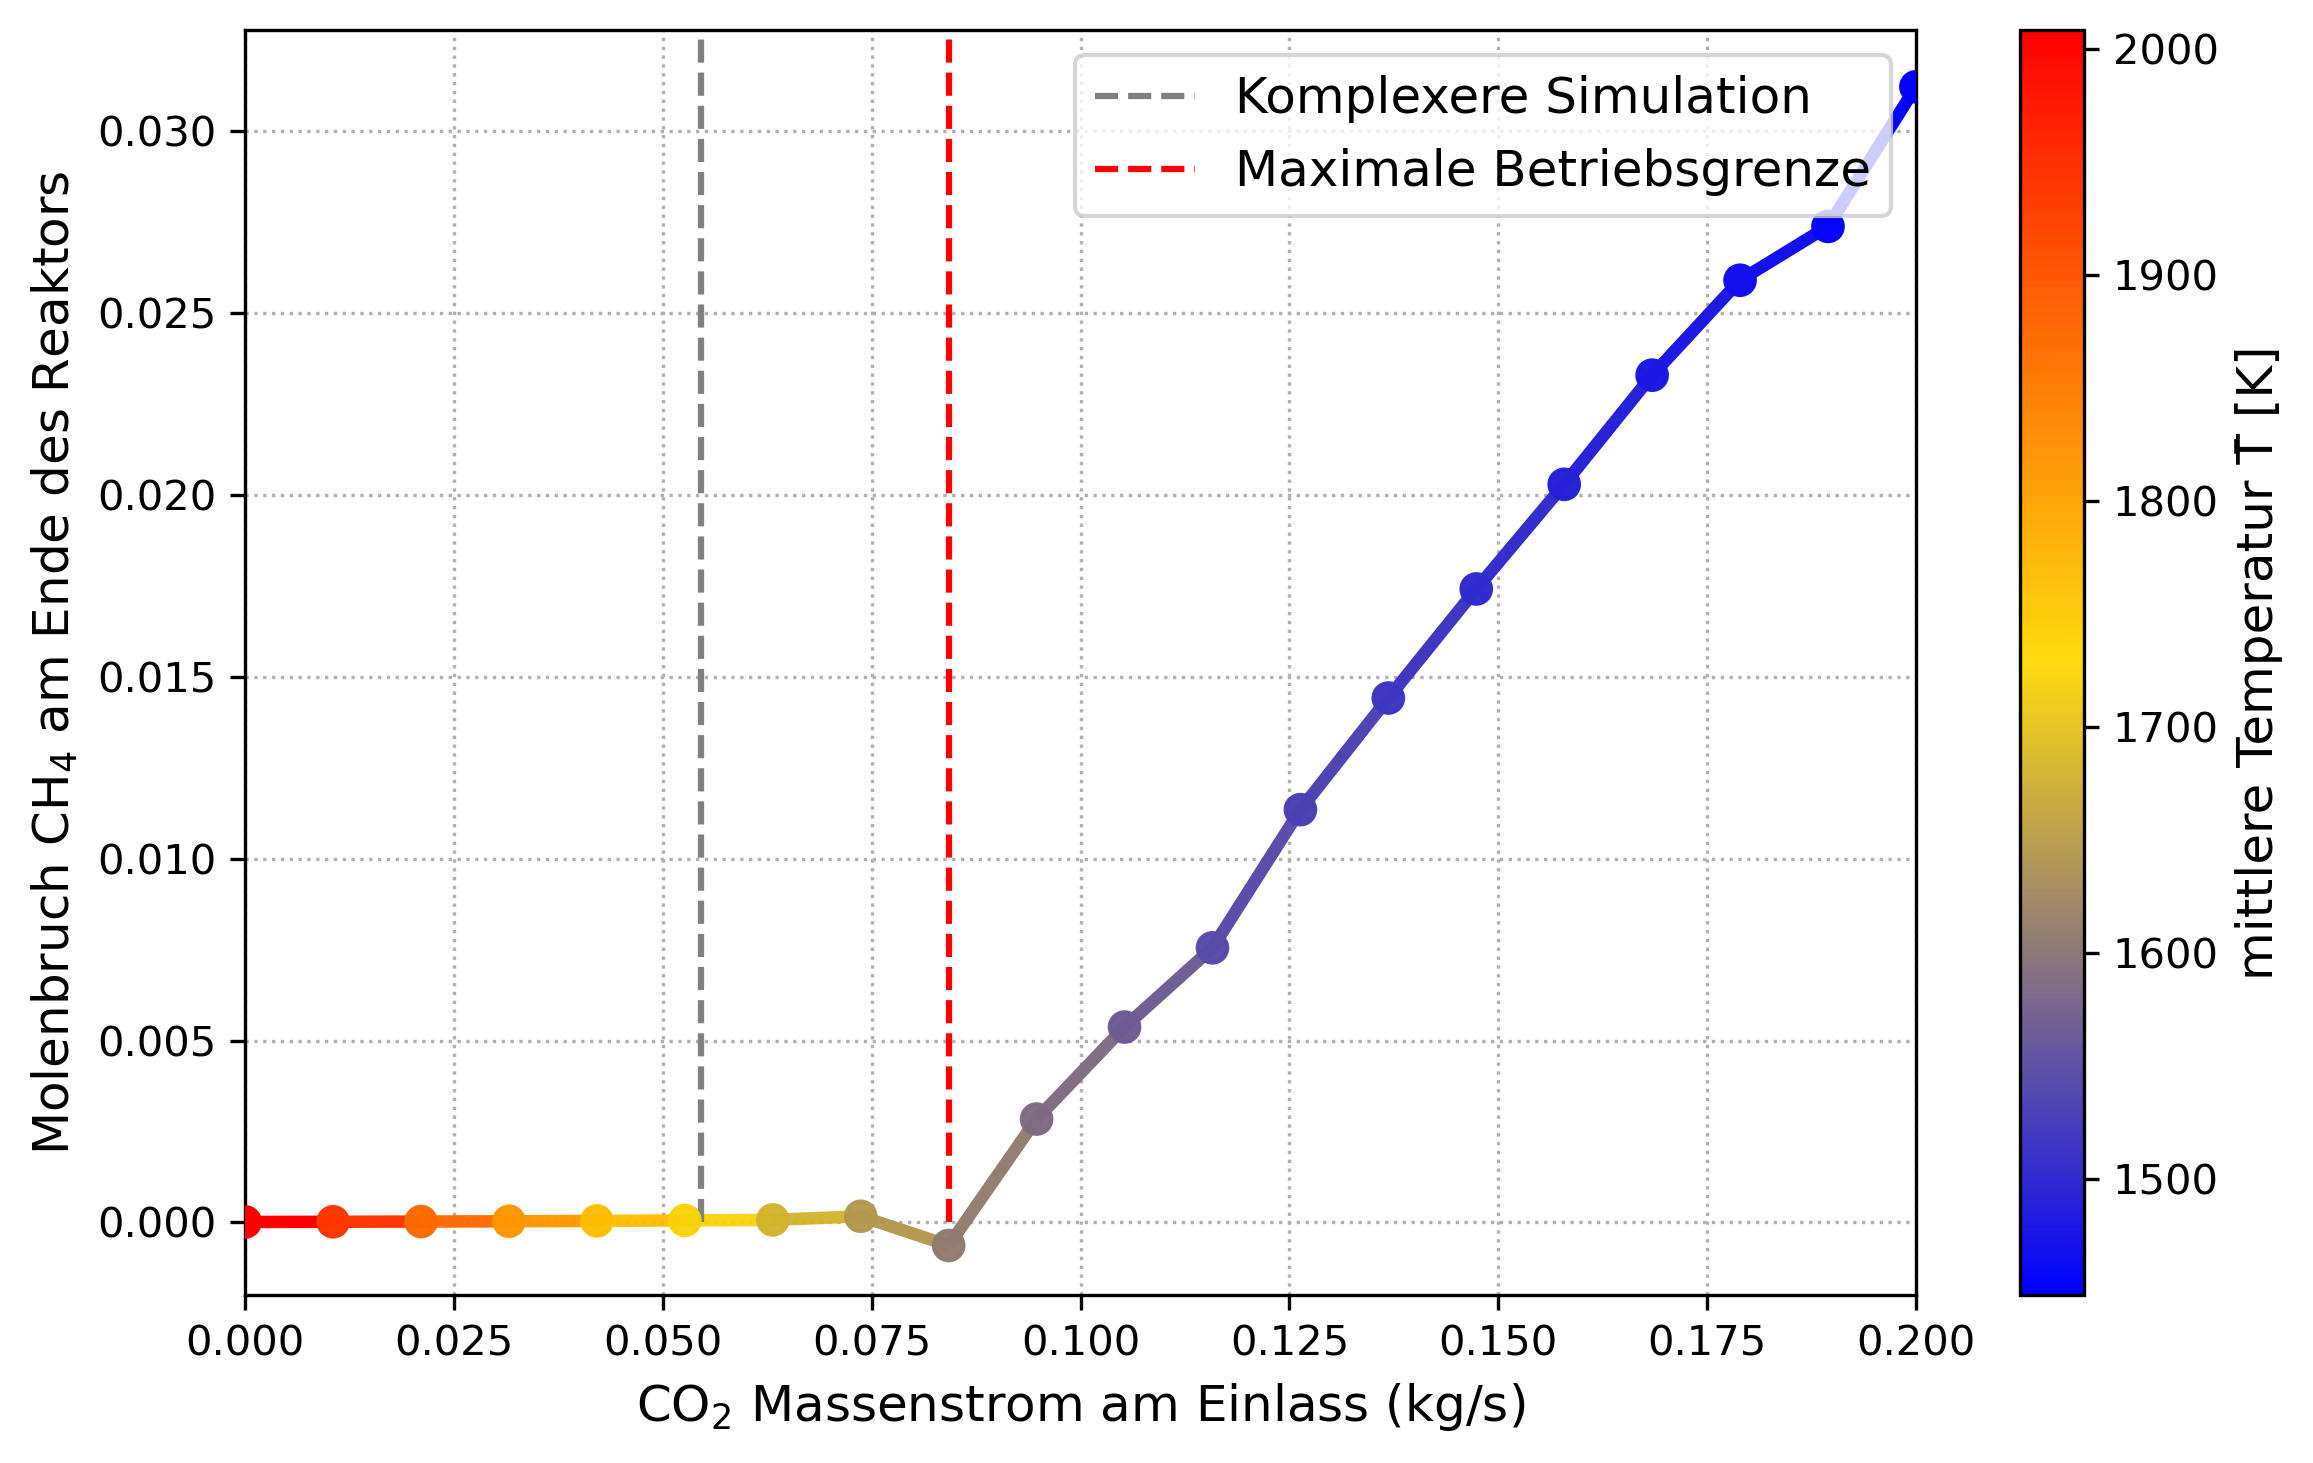
\includegraphics[width=0.75\linewidth]{img/Parameterstudie_CO2/Parameterstudie_CO2_CH4_Schlupf_colormap_marker.png}
            \caption{Methanschlupf und mittlere Temperatur des Reaktors als Ergebnis der Parameterstudie zur Variation des Massenstroms von Kohlenstoffdioxid. Die senkrechte Markierung stellt den Massenstrom im näher betrachteten Fall der POx dar.}
            \label{fig:auswertung_co2_methanschupf}
        \end{figure}
        In Abbbildung \ref{fig:auswertung_co2_methanschupf} ist erkennbar, dass ab einem CO$_2$-Massenstrom von 0,09~kg/s ein linearer Anstieg vorliegt. Dieser lineare Anstieg deutet darauf hin, dass ab dieser Grenze eine erhöhte Zugabe von CO$_2$ eine Umsetzung von Methan direkt verhindert. Dies stellt somit die obere Grenze der Betriebsbedingungen des Reaktors dar. 

        %Dieses Verhalten lässt sich durch mehrere Effekte erklären. Zum einen senkt die Zugabe von CO$_2$ die Temperatur durch eine Erhöhung der Wärmekapazität des Gasgemisches. Gleichzeitig führt eine Verdünnung dazu, dass weniger Sauerstoffmoleküle mit Methanmolekülen reagieren können. Beides sorgt dabei für eine niedrigere Temperatur, wodurch keine vollständige Umsetzung des Methans mehr gegeben ist.

         Dieses Verhalten lässt sich im Wesentlichen durch die Verdünnung des Feeds erklären. Bei Zugabe von Kohlenstoffdioxid muss das umgesetzte Methan eine größere Gasmenge erwärmen, wodurch die Temperatur absinkt. Die niedrigere Temperatur führt wiederum zu einer reduzierten Reaktionsgeschwindigkeit und damit zu einer geringeren Umsetzung von Methan.

        Der erkennbar negative Wert besitzt hierbei keine physikalische Bedeutung, da der Stoffmengenanteil nur Werte im Bereich zwischen 0 und 1 annehmen kann. Diese negativen Werte sind auf numerische Ungenauigkeiten in der Simulation zurückzuführen und entstehen durch Rundungs- und Iterationsfehler bei geringen Konzentrationen. Sie werden daher als numerisches Rauschen interpretiert und auf 0 gesetzt, was einer vollständigen Umsetzung von Methan entspricht. 

        Um sowohl das Ziel der Einsparung von Kohlenstoffdioxidemissionen, als auch die Einbindung in Prozessketten zu ermöglichen, muss ein Betriebspunkt ermittelt werden, bei dem ein hoher Verbrauch von CO$_2$ stattfindet und das Synthesegas ein geeignetes Verhältnisses von Wasserstoff zu Kohlenstoffmonoxid aufweist. Die CO$_2$-Bilanz wird im folgenden als 
        \begin{align}
            X = \frac{\dot m_{out} - \dot m_{in} }{\dot m_{in}} 
        \end{align}
        definiert. Dadurch ergibt sich ein Verbrauch von Kohlenstoffdioxid bei einer negativen Bilanz. In Abbildung \ref{fig:auswertung_co2_bilanz} sind beide beschriebenen Kennzahlen als Ergebnis der Parameterstudie dargestellt. 
        \begin{figure}[H]
            \centering
            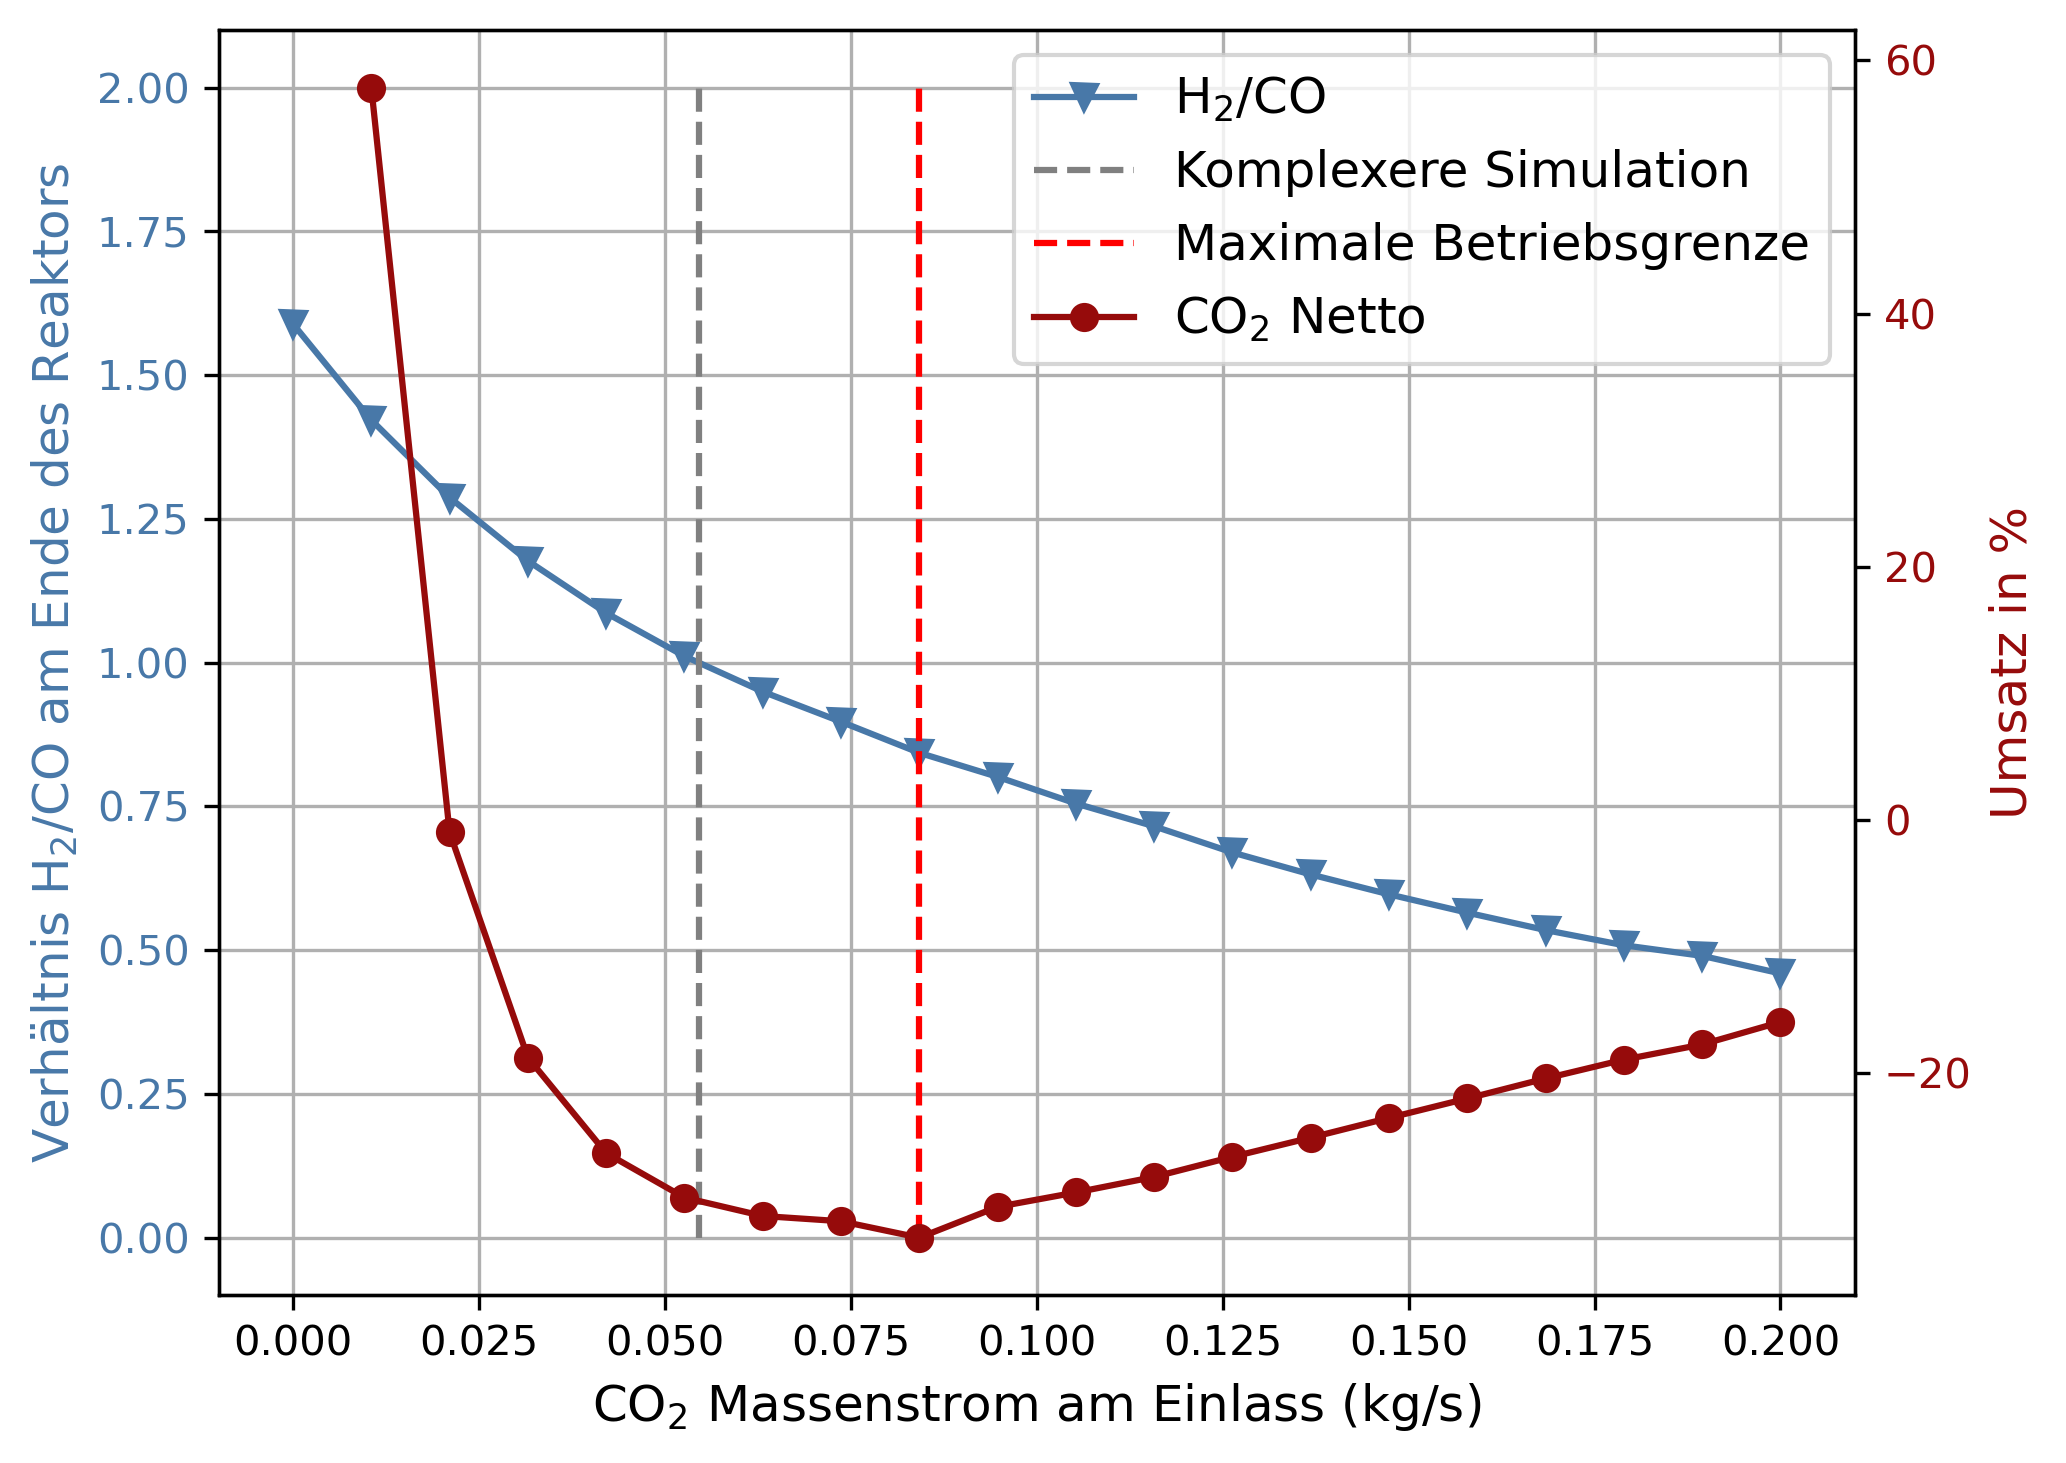
\includegraphics[width=0.75\linewidth]{img/Parameterstudie_CO2/Parameterstudie_CO2_Bilanz.png}
            \caption{CO$_2$-Bilanz und H$_2$/CO-Verhältnis als Ergebnis der Parameterstudie zur Variation des Massenstroms von Kohlenstoffdioxid. Die senkrechte graue Markierung stellt den Massenstrom im näher betrachteten Fall der POx dar}
            \label{fig:auswertung_co2_bilanz}
        \end{figure}
        Mit steigendem Massenstrom steigt der Verbrauch von Kohlenstoffdioxid an, während das H$_2$/CO-Verhältnis kontinuierlich sinkt. Dies ist durch die verstärkte Rückreaktion der Wassergas-Shift-Reaktion erklärbar, da mehr CO$_2$ zu einer Verschiebung des Gleichgewichts führt. Ab der maximalen Betriebsgrenze, ab der das zugeführte Methan nicht mehr vollständig umgesetzt wird, wird auch der Umsatz von Kohlenstoffdioxid geringer. 
        Dieser Trend resultiert aus der Verschiebung des Wassergas-Shift-Gleich\-gewichts in Richtung CO-Bildung.
        \begin{align}
            \mathrm{CO_2 + H_2 \longrightarrow CO + H_2O}
        \end{align}
        Dadurch kommt es sowohl zu einer sinkenden Wasserstoffkonzentration als auch zu einer steigenden Konzentration von Kohlenstoffmonoxid, wodurch sich dieser Trend ergibt. Da für Prozesse wie die Methanolsynthese jedoch Verhältnisse von 2 nötig sind,
        \begin{align}
            \mathrm{CO + 2\ H_2 \longrightarrow CH_3OH}
        \end{align}
        ergibt sich der Bedarf von zusätzlichem Wasserstoff. Die Betriebsparameter aus Tabelle \ref{tab:rahmenbedingungen_versuche} ermöglichen, dass ein H$_2$/CO-Verhältniss von 1 entsteht und gleichzeitig eine negative CO$_2$-Bilanz erzielt wird. 

        Die Ermittlung des Verhältnis Wasserstoff zu Kohlenstoffdioxid unter den Prozessbedingungen stimmt somit mit den Messwerten überein (vgl. Tabelle \ref{tab:messwerte}). Die Abweichung bei dem Referenzfall ist durch die kleine Abweichung an sonstigen Rahmenbedingungen erklärbar.
    \section{Fehlerbetrachtung}
        Alle in der Arbeit genutzten Modelle nutzen in bestimmten Formen Annahmen, die teilweise nicht vollständig bestätigt werden können. Beispielsweise können die Zusammensetzungen und Temperaturen der Feedströme schwanken, Wärmetransport im Reaktor kann durch verschiedene, nicht konvektive Effekte wie Strahlung erfolgen, es gibt eine konstante Kühlleistung, die nicht variiert und viele mehr. Die Messungen der während des Betriebs aufgenommenen Parameter unterliegen Messunsicherheiten und können somit die Auswertung der Modelle mit den geringsten Fehlern beeinflussen. Die Messunsicherheiten sind H$_2 \pm 2\%$, CO$\ \pm\ 2\%$, CH$_4 \pm 5\%$, N$_2 \pm 5\%$ \cite{RICHTER2015110}, was bei sehr nah beieinander liegenden Messergebnissen zu relevanten Abweichungen in den Fehlerwerten führen kann.

        Des Weiteren stellen numerische Lösungen keine analytischen Lösungen dar. Somit können mehrere Fehlerquellen, darunter Approximations- und Rundungsfehler, variierende Ergebnisse verursachen. Da bei umfangreichen Mechanismen schnell Divergenzprobleme auftreten, werden in diesen Fällen Parameter des numerischen Lösungsverfahrens angepasst, was diese Fehlerquellen weiter vergrößert. Da das Lösen von Reaktornetzwerken mit Rückkopplung iterativ erfolgt, wird ein Dämpfungsfaktor verwendet. Eine Verringerung dieses Faktors reduziert zwar die Rechenzeit, erhöht jedoch den numerischen Fehler. Dieser Dämpfungsfaktor stellt damit einen Kompromiss dar und kann für verschiedene Anwendungsfälle angepasst werden, was die Ergebnisse beeinflussen kann.  

        Der mittlere quadratische Fehler (MSE) ist ein gutes Mittel, um simulierte Ergebnisse mit Messergebnissen zu vergleichen und diese Ergebnisse zu bewerten. Allerdings stellt dies keine Möglichkeit dar, Temperatur- und Stoffmengenabweichungen miteinander vergleichen, da sich mit dieser Methode nur Größen einer Größenordnung vergleichen lassen. Ein ähnliches Problem tritt bereits für die Berechnung des Schlupfs von Methan auf, da dieser Stoffmengenanteil eine deutlich kleinere Größenordnung als die Vergleichsstoffe darstellt. Eine Wichtung verschiedener Stoffe kann dieses Problem vermindern, allerdings ist diese Wichtung empirisch und muss wieder unter Zuhilfenahme verschiedener Annahmen überprüft werden. 
    \chapter{Fazit und Ausblick}

    In dieser Arbeit wurde gezeigt, dass die nichtkatalytische Partialoxidation von Erdgas bereits durch einfache, reduzierte Modelle, bestehend aus lediglich zwei idealisierten Reaktoren, präzise abgebildet werden kann. Selbst eine einfache lineare Verknüpfung eines PSR und eines PFRs führte zu Simulationsergebnissen mit geringer Abweichung von den experimentellen Messwerten. 
    Eine noch höhere Genauigkeit der Simulationsergebnisse ließ sich durch das Hinzufügen idealisierter Reaktoren zum bestehenden Netzwerk erreichen, die Strömungsphänomene im Reaktor gesondert abbilden. Dabei zeigte sich jedoch, dass in einem einfachen Reaktor, wie in dieser Arbeit betrachtet, eine grobe Aufteilung des Reaktors besser funktioniert als eine detailreiche Reaktorsegmentierung. Diese detailreiche Segmentierung müsste zuerst durch eine CFD-Analyse abgebildet werden, wodurch sich falsche Annahmen für Rahmenbedingungen in die Simulation des ROMs fortpflanzen würden. Als Folge liefert ein mittelmäßig komplexes Modell den geringsten Fehler. 

    Die oft in der Literatur vorgefundenen Aussagen, dass moderne Reaktionsmechanismen zu vergleichbaren Ergebnissen führen und die Genauigkeiten der genutzten Mechanismen stark von Randbedingungen abhängen, konnten durch eigene Simulationen bestätigt werden. Außerdem konnte die These gestützt werden, dass die Mechanismen für die trockene Reformierung größere Abweichungen liefern als für die herkömmliche POx, da wesentlich bestimmende Reaktionen in diesen Reaktionen nicht ausreichend parametrisiert sind. Dies ist jedoch nicht die alleinige Ursache diese Unterschiede.

    Obwohl für die Entwicklung dieser reduzierten Reaktormodelle eine CFD-Analyse notwendig war, konnte aus den Ergebnissen ein Modell mit hoher Modellgüte entwickelt werden, das mit hoher Effizienz wesentliche Vorgänge präzise abbilden kann. Auf der Grundlage dieses validierten Modells können umfangreiche Parameterstudien durchgeführt werden, und eine Anwendung in der Echtzeitregelung ist denkbar.

    Sollte sich dieser Prozess als Möglichkeit zur Nutzung von Prozessgebundenem Kohlenstoffdioxid im großindustriellen Maßstab beweisen, ist zukünftig mit einem verstärkten Fokus auf die Entwicklung in diesem Bereich zu rechnen, was zur Entwicklung eines für diesen Prozess optimierten Reaktionsmechanismus führen könnte. Auch ist zukünftig die Entwicklung reduzierter Modelle mittels datengestützter Verfahren (z.B. künstliche Intelligenz) denkbar. Obwohl die Rechenleistung immer weiter zunimmt, werden CFD-Simulationen nicht in der Lage sein, komplexe Optimierungsaufgaben solcher Reaktoren durchzuführen. Aus diesem Grund wird die Entwicklung reduzierter Modelle zukünftig einen wichtigen Teil in der Entwicklung neuer Prozesse bzw. Prozessbedingungen spielen. 
    \printbibliography
\end{document}

---------- 19.09. -----------------
CH4 schlupf parameterstudie
2 - 3 Simulationen rezirkulaitonsverhjältnis
Temperatur an und vergleichen (+PP)
Rechenzeiten 

----------- Ideen 3D Plots --------
Parameterstudie: CO2 inlet und Profil PFR unten, nach oben Temperatur 

--------- 21.10. ----------
Farben für Plots okay?
MSE sinnvoll? was sonst?
Quellen ausreichend?
Theorie genug / zu viel? Mehr Tiefe in MSE / anderes?
Plots für Parameterstudie zu einfach?
Darstellungen ROMs okay?
Rechenzeiten schlecht messbar durch Dämpfung sehr willkürlich
Anhang? Wenn ja, womit? Wertetabellen, Plots,..?


mit co2: kürzere VWZ 
CO2-Bilanz Prozentual 
Abstand zwischen Säulen im Diagramm